\documentclass[18pt]{report}
\usepackage[paperheight=11in, paperwidth=8.5in, left=1.5in, right=1in, top=1in, bottom=1in]{geometry}
%\usepackage[a6paper,margin=0.4cm]{geometry}
\usepackage{newunicodechar}
\newunicodechar{fi}{fi}
\newunicodechar{ff}{ff}
\usepackage{graphicx}
\graphicspath{ {images/} }
\usepackage[sorting=none]{biblatex} 
\addbibresource{reference.bib} % maintained by hand
\addbibresource{references.bib} % direct import from Mendeley
\usepackage[version=4]{mhchem}
\usepackage[ampersand]{easylist}
\usepackage{amssymb}
\usepackage{amsmath}
\usepackage{mathtools}
\usepackage{chngcntr}
\counterwithout{figure}{chapter}
\counterwithout{table}{chapter}
\setcounter{tocdepth}{3}
\setcounter{secnumdepth}{3}
\usepackage[document]{ragged2e}
\usepackage{xifthen}
\usepackage[english]{babel}
\newcommand{\oneline}[1]{%
  \newdimen{\namewidth}%
  \setlength{\namewidth}{\widthof{#1}}%
  \ifthenelse{\lengthtest{\namewidth < \textwidth}}%
  {#1}% do nothing if shorter than text width
  {\resizebox{\textwidth}{!}{#1}}% scale down
}

\usepackage{indentfirst}
\usepackage{tocloft}
\usepackage{notoccite}
\usepackage{appendix}
\usepackage{fancyhdr}
\usepackage[T1]{fontenc}
\usepackage{abstract}
\usepackage{pbox}
\usepackage{array}
\usepackage[table]{xcolor}
\setlength{\arrayrulewidth}{1mm}
\setlength{\tabcolsep}{18pt}
\addto\captionsenglish{\renewcommand{\arraystretch}{1.5}}
\newcolumntype{s}{>{\columncolor[HTML]{AAACED}} p{3cm}}
\usepackage{adjustbox}
\usepackage{chemfig}
\usepackage{xymtexps}
\usepackage{xymtexpdf}
\usepackage{xcolor}

\usepackage{hyperref}
\hypersetup{
    colorlinks=true,
    linkcolor=blue,
    filecolor=magenta,
    urlcolor=cyan,
}


\defbibheading{bibliography}[\bibname]{%
  \chapter*{\centering #1}%
  \markboth{#1}{#1}}
  
% \addto\captionsenglish{\renewcommand{\bibname}{REFERENCES}}
% \addto\captionsenglish{\renewcommand{\thefigure}{\arabic{chapter}.\arabic{figure}}}
% \setcounter{figure}{0}

% \let\listoffigures\listoffigures



\addto\captionsenglish{\renewcommand{\abstractname}{\hfill\bfseries\Huge ABSTRACT\hfill}} 
\addto\captionsenglish{\renewcommand{\cftaftertoctitle}{\hfill}}
\setlength{\absleftindent}{0pt}
\setlength{\absrightindent}{0pt}

\addto\captionsenglish{\renewcommand{\contentsname}{\hfill\bfseries\Huge TABLE OF CONTENTS\hfill}} 
\addto\captionsenglish{\renewcommand{\cftaftertoctitle}{\hfill}}

\addto\captionsenglish{\renewcommand{\listfigurename}{\hfill\bfseries\Huge LIST OF FIGURES\hfill}} 
\addto\captionsenglish{\renewcommand{\cftaftertoctitle}{\hfill}}

\addto\captionsenglish{\renewcommand{\listtablename}{\hfill\bfseries\Huge LIST OF TABLES\hfill}} 
\addto\captionsenglish{\renewcommand{\cftaftertoctitle}{\hfill}}


\addto\captionsenglish{\renewcommand{\bibname}{\hfill\bfseries\Huge REFERENCES\hfill}} 
\addto\captionsenglish{\renewcommand{\cftaftertoctitle}{\hfill}}

\addto\captionsenglish{\renewcommand{\appendixtocname}{APPENDIX}}

\makeatletter
\addto\captionsenglish{\renewcommand{\thereaction{Reaction\,\thechapter.\arabic{reaction}}}}
\newcounter{reaction}
\newcommand\reactiontag%
  {\refstepcounter{reaction}\tag{\thereaction}}
\newcommand\reaction@[2][]%
  {\begin{equation}\ce{#2}%
  \ifx\@empty#1\@empty\else\label{#1}\fi%
  \reactiontag\end{equation}}
\newcommand\reaction@nonumber[1]%
  {\begin{equation*}\ce{#1}\end{equation*}}
\newcommand\reaction%
  {\@ifstar{\reaction@nonumber}{\reaction@}}
\makeatother

\pagestyle{fancyplain}
\fancyhf{}
\fancypagestyle{plain}{\thispagestyle{fancy}} 
\fancyhead[R]{\thepage}
\addto\captionsenglish{\renewcommand{\headrulewidth}{0pt}}
\addto\captionsenglish{\renewcommand{\abstractname}{ABSTRACT}}
% \defbibheading{bibliography}[\bibname]{\centering}
\usepackage{atbegshi}% http://ctan.org/pkg/atbegshi
\AtBeginDocument{\AtBeginShipoutNext{\AtBeginShipoutDiscard}}

\begin{document}
\begin{titlepage}
   \begin{center}
       \Large{AUTOMATED GENERATION OF CHEMICAL KINETIC MECHANISMS OF FISCHER-TROPSCH (F-T) 
       GAS-TO-LIQUID FUEL SURROGATES}
       \vspace{1.5cm}
       \large
\vspace{2cm}

       A Thesis Presented\\
            \vspace{0.5cm}
                By\\
                \vspace{0.5cm}
        \text{Chikpezili Ebubechukwu Ajulu}\\
        \vspace{0.5cm}
                    to\\
                    \vspace{0.5cm}
                    
     
\centering The Department of Mechanical \& Industrial Engineering 
\vspace{0.5cm}
       
\centering            in partial fulfillment of the requirements\\ 
            \vspace{0.15cm}
                    for the degree of\\
                    \vspace{0.5cm}
                    
                    \Large{Master of Science}\\
                    \vspace{0.5cm}
                        in the field of\\
                        \vspace{0.5cm}
                        Mechanical Engineering\\ 
                    with a concentration in Thermofluids
 
       \vspace{0.8cm}
 
       %\includegraphics[width=0.4\textwidth]{Northeastern University}
 
       \LARGE
       Northeastern University\\
       Boston, Massachusetts\\
       \vspace{0.5cm}
       \large{May 2020}
       \vspace{1.25in}
 
   \end{center}
\end{titlepage}

\pagenumbering{roman}

% \thispagestyle{plain}


    
    \justifying

             
    Environmental pollution as a result of continued fossil fuel usage has long been a bone of contention especially in the energy industry, particularly around transportation fuels. Transportation fuels, precisely jet fuels have long been studied to curb the production of harmful byproducts from the combustion of these fuels by proposing new jet fuel synthesis. Researchers have invested resources to the synthesis of alternative jet fuels that promise lower emissions of harmful gases such as NOx, SOx and particulates. Studies and research have yielded in the fruition of a catalytic process that involves the conversion of already existing gas-to-liquid fuels via the Fischer-Tropsch (F-T) synthesis for jet fuels that promise lower emissions. As a result of these strides, the oxidation of these alternative jet fuels is pertinent especially for new engine designs. Surrogate modeling of the F-T GTL fuels is proposed based on spectrometry analysis to determine the major components of the F-T GTL fuel.
    
    This study is done on the automated chemical kinetic mechanism generation and validated analysis of a three-component F-T GTL fuel surrogate chemical kinetic model, comprising of three primary reference fuels (PRFs); n-decane, iso-octane and n-propyl-cyclohexane. The detailed chemical kinetic mechanism of the three-component fuel blend is constructed using the open-source software for automated chemical kinetic mechanism generation, Reaction Mechanism Generator (RMG). Comparison between the concatenation of the PRFs was compared to a kinetic model that consists of the direct generation of the PRF species when lumped together from the onset for cross-reactions in RMG. 
    
    Further analysis and model validation was carried out using an open-source software for solving chemical kinetic, thermodynamic and transport problems, Cantera. The chemical kinetic models are analyzed and compare the auto-ignition characteristics (ignition delay time) to that of experimental measurements of the GTL fuels at a wide range of conditions as well as to other chemical kinetic models of the PRFs before concatenation and the GTL lumped fuel surrogate model. The computational comparison is made for the best framework in constructing a detailed GTL fuel surrogate chemical kinetic model as well as which approach is best suited to closely match experimental validation.

\thispagestyle{empty}
\chapter*{\centering ABSTRACT}
\thispagestyle{plain}


    
    \justifying

             
    Environmental pollution as a result of continued fossil fuel usage has long been a bone of contention especially in the energy industry, particularly around transportation fuels. Transportation fuels, precisely jet fuels have long been studied to curb the production of harmful byproducts from the combustion of these fuels by proposing new jet fuel synthesis. Researchers have invested resources to the synthesis of alternative jet fuels that promise lower emissions of harmful gases such as NOx, SOx and particulates. Studies and research have yielded in the fruition of a catalytic process that involves the conversion of already existing gas-to-liquid fuels via the Fischer-Tropsch (F-T) synthesis for jet fuels that promise lower emissions. As a result of these strides, the oxidation of these alternative jet fuels is pertinent especially for new engine designs. Surrogate modeling of the F-T GTL fuels is proposed based on spectrometry analysis to determine the major components of the F-T GTL fuel.
    
    This study is done on the automated chemical kinetic mechanism generation and validated analysis of a three-component F-T GTL fuel surrogate chemical kinetic model, comprising of three primary reference fuels (PRFs); n-decane, iso-octane and n-propyl-cyclohexane. The detailed chemical kinetic mechanism of the three-component fuel blend is constructed using the open-source software for automated chemical kinetic mechanism generation, Reaction Mechanism Generator (RMG). Comparison between the concatenation of the PRFs was compared to a kinetic model that consists of the direct generation of the PRF species when lumped together from the onset for cross-reactions in RMG. 
    
    Further analysis and model validation was carried out using an open-source software for solving chemical kinetic, thermodynamic and transport problems, Cantera. The chemical kinetic models are analyzed and compare the auto-ignition characteristics (ignition delay time) to that of experimental measurements of the GTL fuels at a wide range of conditions as well as to other chemical kinetic models of the PRFs before concatenation and the GTL lumped fuel surrogate model. The computational comparison is made for the best framework in constructing a detailed GTL fuel surrogate chemical kinetic model as well as which approach is best suited to closely match experimental validation.

\addcontentsline{toc}{section}{\abstractname}

\cleardoublepage
\chapter*{\centering ACKNOWLEDGMENTS}
\thispagestyle{plain}

\justifying


As with all things in life, all good things come to an end. This is the end of my journey at Northeastern University after six eventful years of growth, learning and immense experience with amazing people. I like to thank God for life, my parents - Dennis and Ifeoma whose prayers, emotional support and resources have brought me this far I remain blessed thank you for everything both professional, parental and spiritual. My siblings; Kachi, Ijem and Nchedo especially, Nchedo he's been an amazing brother and friend. I also want to mention Obehi, he has become family,  a confidant and brother whose guidance especially in navigating the difficult terrain of the professional world has been invaluable. My mentor Prof. Marilyn Minus has been a rock throughout my time at Northeastern. She has always encouraged me and given me the advice to keep fighting despite the challenges. I am also very happy to have met Prof. Andrew Gouldstone, who introduced me to Prof. Minus he's jovial yet has an amazing ability to convey excellent analysis and sit down to interact with just about anyone. It is something I have always loved about him and admire. Prof. Kowalski, he was someone who saw talent in me and helped me nurture it through close interactions and eventually convincing me to stay in grad school. I'll like to also mention Prof. Smyser, she is an amazing person and I hope to work with people like her. She showed me empathy in leadership and how to appreciate the people you work with even if they're direct reports. I always marvelled at the thought of how she cared for her grad students by the timely Christmas gift cards year after year. Also, Kevin McCue was someone I got to know and respect. We had close interactions and he made me confident in front of students as a TA, his pragmatic approach to problem solving really helped shape me as an engineer. 

In MIE I have never met somone as impressionable as Prof. Mehdi Abedi, his love and passion for science pushed me to the brink. Likewise his sometimes encouraging words. Prof. Metghalchi was my advisor you were kind and gracious I always recall the first time we met and how you always reminded us to use the right lingo when discussing energy and it's become a lifestyle I like to imbibe. Prof. Levendis, after we met you impressed me with your style and sense of fashion, your dedicated passion for combustion pushed me to learn about gas turbine combustion and we've become life long friends and I always cherished being able to walk into your office to discuss about combustion thank you for the memories. 

Prof. Michael Allshouse thank you so much for the exposure you gave me I never believed I would be able to code and here I am writing a thesis about code generation in chemical kinetics. Thank you for your kind words even when we meet at church you and Nina are always so welcoming. You made me love CFD despite it being the hardest class I took, you made me like your ability to debug code and interpret what the solver was doing, a very methodological approach. 

Prof. Richard West, thank you so much. This thesis is really all about your help for the last two years. I know how I met you and got frustrated not knowing what to work on yet you persisted and pushed me beyond my abilities. Because of your guidance I learned to like chemistry and kinetics again. I know deep down I did frustrate you as a student but you never gave up on me. Thank you for introducing me to RMG and the Cantera team with Dr. Ray Speth, Prof. DeCaluwe, Prof. Bryan Weber, Prof. Kyle Niemeyer as well as chemical kinetics I do hope to become as proficient at coding as you one day. To the CoMoCheng group Nate, Krishna, Emily, David, Chris, Shenghui and Chao you all contributed passively to me learning in one way or the other I hope to form the bond you all share. To the MIT RMG team especially, Matt Johnson, you'll forever be in my heart your graciousness to always teach and explain code and debug issues in RMG made this thesis possible and Max Liu and Mark Payne. Thank you for the late night responses, impromptu visits and calls. Dr. Richard Marsh at Cardiff University who sparked my interest in combustion thank you for this gift.

To my close friends who pushed me harder than they could imagine Nneoma, Emmanuel, Oseghale, Uzoma for helping me out with python and data science, Natasha and my recent but go to workout mentor, my wonder woman Chinenye you pushed me harder than I could imagine and provided the emotional support to go through it all. I remain grateful. To the podcasts from Ravi Zacharias, Steven Furtick, Pastor Jan, Pastor Sola Osunmakinde my Back Bay CG at Mosaic, those podcasts and messages lifted my spirit in times of despair thank you. 

To anyone who'll ever read this thesis, be encouraged to never despair in times of hopelessness and adversity even when all hopes seem lost, continue striving for it is through our steepest moments of uncertainty is our greatest work conceived. Thank you to all my teachers from primary school to secondary school and at Oxbridge for the investment over the years. It was an honor to have learned from you all.\cleardoublepage
\tableofcontents
\cleardoublepage
\listoftables
\cleardoublepage
\listoffigures
\cleardoublepage

\pagenumbering{arabic}



\justifying
\chapter{Introduction}
\section{Background}
% \label{chap:introduction}
Environmental pollution has long been the subject of discussion in the energy and transportation industry, both among policy makers, industry professionals and researchers alike. The continued use of fossil fuels over the decades, in the form of coal, oil and natural gas for a plethora of applications such as power generation, transportation, industrial and large scale manufacturing processes has seen the gradual deterioration of air quality and life \cite{EnergyInformationAdministration2018U.S.2017}.

In recent times, especially in the power generation sector, the use of generative gas turbines for electricity has been preferred over nuclear fuel due to the dire consequences nuclear energy possesses. Nonetheless, the use of gas turbines has not been without its setbacks; its harmful effects particularly, as relates to pollution and emissions from heavy duty fuels, in the form of \ce{SO2}, \ce{NO} and gaseous hydrocarbons \cite{Timko2010ParticulateFuel}. As a result of the policy to curb carbon emissions in and greenhouse gases (GHG), there has been increasing attention to the research of reducing carbon emissions in jet fuels for aero-derivative gas turbine engines \cite{Timko2010ParticulateFuel}. While traditional fossil fuels account for 81\% of US energy demands, it is expected to fall in the near future with the rise of new renewable technologies \cite{EnergyInformationAdministration2018U.S.2017}. 

\begin{figure}[ht]
    \centering
    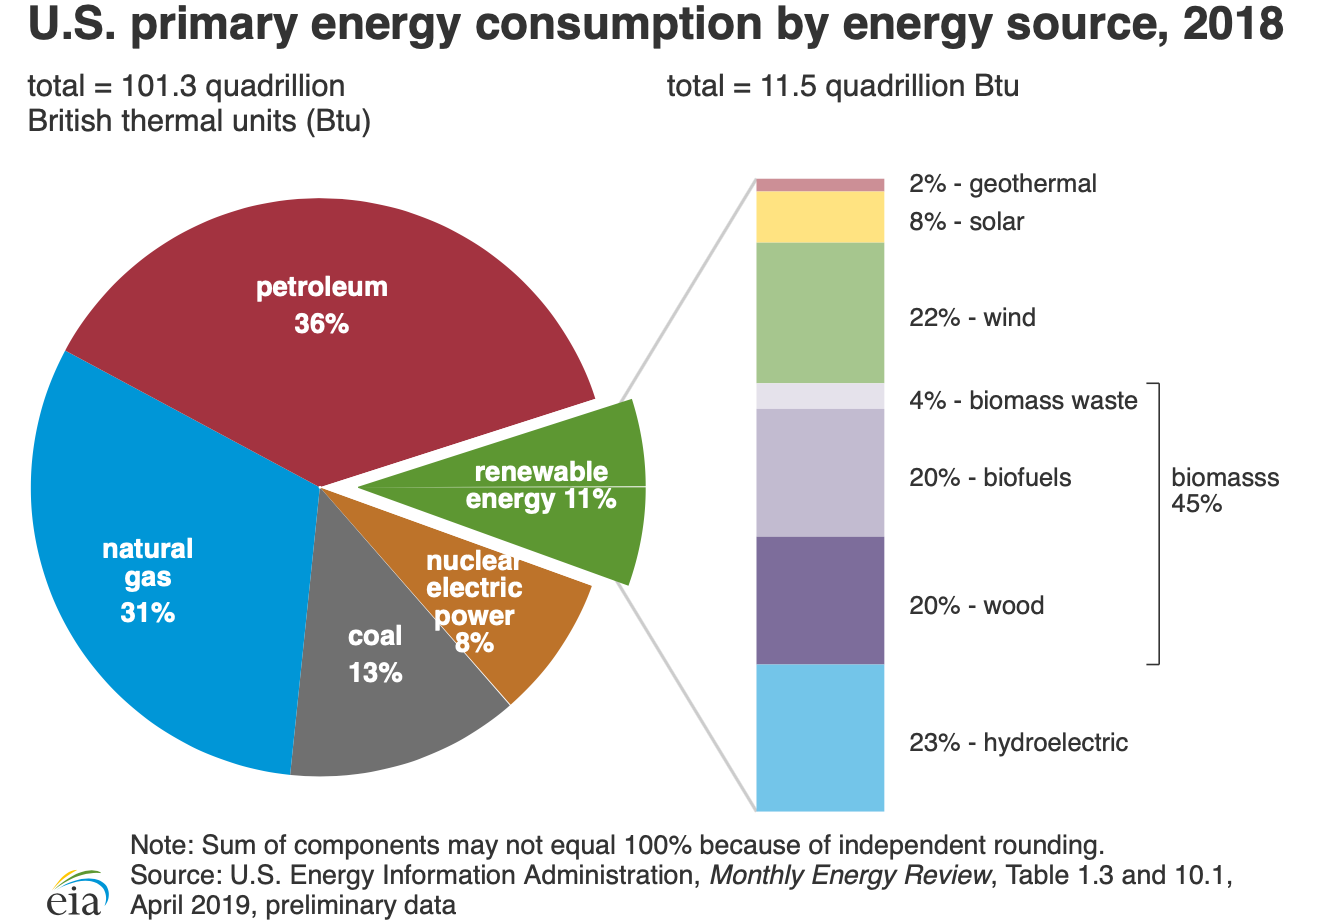
\includegraphics[width=\textwidth, height=\textheight, keepaspectratio]{images/chart-2.png}
    \caption{U.S. primary energy consumption by energy source, 2018 \cite{EnergyInformationAdministration2019Monthly2019}}
    \label{fig:energy demand}
\end{figure}


Notwithstanding, the reliance of power generation on fossil fuels particularly in the heavy duty and aviation industry is without a match at the moment and for some time to come \cite{NationalsAcademiesofSciences2016CommercialResearch}. In lieu of these facts, it is pertinent to abound and comply with emission and pollution regulations designed to curb harmful byproducts of fossil fuels for power generation and transportation by the research, modeling and adoption of alternative non-petroleum based fuels. 

The transportation industry, especially air transport, has long been powered by traditional fossil fuels commonly known as jet fuel. Jet fuels typically consist of carbon-carbon bonded chains blended together with other mixtures. The traditional jet fuels used in commercial air transport typically consist of Jet-A1,JP-8 and JP-10 \cite{NationalsAcademiesofSciences2016CommercialResearch}. These traditional jet fuels however, consist of harmful blends that have the tendency to increase emissions levels and go beyond the limits set by the regulatory environmental agencies. Most of these traditional fuels consist of aromatics that induce particulate matter as well as other volatile organic compounds in the environment and can decrease the life cycle of jet engines based on the refining processes employed \cite{Corporan2007EmissionsFuel}. As a result, efforts have been made to introduce alternative jet fuel blends such as Fischer-Tropsch (F-T) fuels in commercial and military aviation. 

The alternative jet fuels are being synthesised based on mass spectrometry and chromatography analyses to observe the composition of the main driver species behind the high emissions level. The alternative fuels already being used are economical in the sense that, they do not require the extra cost of re-designing existing engines but can be retrofitted to serve as drop in fuels to existing engines \cite{NationalsAcademiesofSciences2016CommercialResearch}. 

\section{Motivation}
Traditional jet fuels typically have \ce{NOx}, \ce{SOx} and particulate matter, but with improved catalytic and synthesis processes, these fuels can be derived from lower carbon fules such as methane or synthesised processes, free of sulphur, nitrogen and contain very little to no aromatics that cause soot \cite{Boogaard2017ToxicologicalToxicology}. There are existing alternative transportation fuels that promise reduced emission such as Liquefied Natural Gas (LNG) fuels, oxygenated fuels such as dimethylether (DME) and other sustainable alternative jet fuels. These alternative jet fuels are being derived through various synthesis and catalytic processes to produce fuels that promise reduced emissions and carbon concentration to the environment\cite{Whale2018ToxicologicalEcotoxicology}. The sustainable aspect refers to the push for fuels that reduce pollution and emissions with a goal of having little to no pollutants, while alternative refers to the method and processes used to refine the fuel - non-petroleum based processes \cite{NationalsAcademiesofSciences2016CommercialResearch}. 

One of the commonly used alternative jet fuels already being used in circulation is the Gas-to-Liquid alternative jet fuel. They are derived from natural gas as feedstock and synthesised through the Fischer-Tropsch (F-T) \cite{Speight2014ChapterProcess} Process in the presence of catalysts to remove unwanted mixtures such as \ce{CO} in the fuels. GTL fuels promise lower \ce{CO2} emissions and can still be used in existing engines without the need to redesign the engines \cite{Corporan2007EmissionsFuel}. Most importantly, these alternative jet fuels (GTL fuels) comply with the existing regulations for emissions and pollution limits for jet fuels as they are already being used both as primary jet fuels and being blended with other compounds to achieve the desired regulatory limits for jet fuel emissions. 
\cleardoublepage
\section{Fischer- Tropsch Gas-to-Liquid (GTL) Fuels}
Gas-to-Liquids (GTL) are essentially catalytic processes that take existing natural gases through either a Methanol synthesis or Fischer-Tropsch (F-T) synthesis. This work is focused on the recovery of GTL through the F-T synthesis to obtain longer carbon chain with high energy content such as gasoline, jet fuel and diesel fuels in the carbon-carbon bonds \cite{U.S.EIA}. The chemistry of the F-T process is a catalytic chemical reaction that was developed in Mülheim an der Ruhr, Germany at the Kaiser Wilhelm Institut für Kohlenforschung by Franz Fischer and Hans Tropsch. This process was named after the inventors and is known as the ‘Fischer–Tropsch process’ \cite{Boogaard2017ToxicologicalToxicology}.
It involves the reaction of carbon monoxide \ce{CO} and hydrogen \ce{H2} in syngas conversion to hydrocarbons of various molecular weights. Controlled by the chemical equation:

  \reaction{(2n + 1) H2 + nCO \longrightarrow C_n H_{2n+2} + nH2O }

Where $n$ is an integer, and when $n$=1, it indicates methane being formed, which is often thought to be an unfavorable byproduct. This reaction also produces significant byproducts such as the water-gas-shift reaction. 
\reaction{CO + H2O \longrightarrow H2 + CO2 }

\begin{figure}[ht]
    \centering
    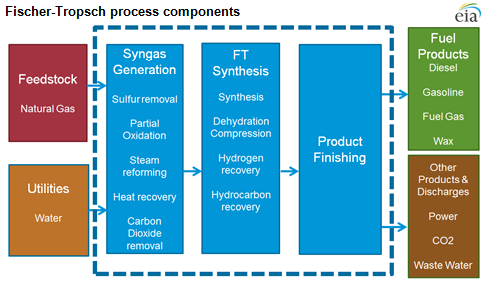
\includegraphics{images/chart2.png}
    \caption{Fischer-Tropsch Synthesis \cite{Mallik2014Gas-to_liquidsMarket}}
    \label{fig:F-T synthesis}
\end{figure}
The conditions typically chosen for the F-T synthesis is made such that there is formation of large hydrocarbons in the presence of catalysts such as Nickel \ce{Ni},Iron\ce{Fe},Cobalt\ce{Co} and Ruthenium \ce{Ru}. While Nickel tends to favor the formation of methane \ce{CH4}, Iron is more economical and also guarantees a higher water-gas-shift activity, it is more suitable when there is low hydrogen/carbon monoxide ration in the syngas such as that in coal gasification \cite{Schulz1999ShortSynthesis}. This process is typically referred to as Reforming \cite{Boogaard2017ToxicologicalToxicology}. This reforming process eliminates harmful vapors that are can cause damage to engines and the environment when combustion occurs. 


These GTL fuels can also serve as alternatives to traditional diesel fuels and heavy carbon fuels, like fuel oils used in heavy machinery based on the low emissions and pollution levels \cite{Timko2010ParticulateFuel}. Since these GTL fuels are going to be used in existing engines. It is imperative to understand the physical and chemical properties of these fuels under engine-like conditions to order to continue the adoption of these fuels as sustainable alternative replacements to traditional jet fuels derived from petroleum-based processes. Furthermore, since engine designers need fuel models as close to the real physical fuel as possible, in order to make real-life simulations of fuel reactivity under engine-like condition, methods like computational fluid dynamic (CFD) model engines are employed to predict the thermal stresses, deformation, fatigue and transport characteristics of these fuel. Thus, it is imperative to look at the possibility of researching fuel models known as chemical kinetic mechanisms that closely represents the real fuel under engine-like conditions as well as the elementary reaction pathways that occur when such fuels are used.


\section{Surrogate Models}
\subsection{What are Surrogate Models ?}
Surrogate models are easily interpretable models of complex physical systems typically used in engineering applications where direct analysis of a system, variables or outcome cannot be measured explicitly \cite{molnar2019}. 
Over the course of the last few decades, surrogate modeling in the form of numerical approximations has become more computationally expensive as the technological advances in computing improves, due to the more demand on making more numerical models that closely match physical systems. This has made engineering tasks more demanding and longer to complete as more fields in system optimization employ these techniques. These surrogate models are often used to significantly reduce both the computational cost and time for numerical approximations. Surrogate models employ the unique technique of evaluating an original function or model at approximate points based on mathematical or physical deductions of the system behavior. Since surrogate modeling is at the heart of numerical optimization, it is often used as a means to deduce what consists of a complex physical system as well as its behavior. Within surrogate modeling optimization, derivatives are often imposed, since optimization usually requires gradient-based algorithms for efficacy and approximate solutions \cite{Bouhlel2019ADerivatives}. These derivatives in the context of chemical systems, require the use of mass spectrometry to determine what constitutes a complex system.

\subsection{Why Surrogate Models ?}
Engine designers of heavy duty machinery especially gas turbines, generally develop new designs of gas turbines through the use of computational models\cite{Mehl2012ModelingApproach}. These computational models involve the use of mathematical representations of physical systems. For engines, as a result of the mechanism for power generation in internal combustion engines (IC), designers and engineers use multi-physics based models of fluid flow to integrate both mass, heat and chemical kinetic models together for a holistic and robust approximation of the physical system through the implementation of computational fluid dynamic (CFD) calculations. These models are usually performed in order to optimize and characterise emission and pollution levels. In order to do this for IC engines, it is pertinent to include the complex chemical reaction pathways involved in the realization of these models. 

\subsection{Surrogate modeling in chemical kinetic mechanisms of fuels}
Chemical reactions of transportation fuels involve large chemical compounds consisting of hundreds and thousands of chemical species, which would prove to be physically impossible to model individually. As such a lumped representation of the large complex chemical compounds can be used to model what is the resulting overall fuel compound. This method of using a lumped representation of complex physical and chemical systems is known as surrogate modeling. 

GTL fuels are blended fuels with a combination of varieties of other pure primary reference fuel compounds based on spectrometry analyses. In order to represent this blended fuel model it is important to know the primary composition of this fuel. Many alternative jet fuels have been used in recent times such as the F-T derived and biomass derived alternative jet fuel surrogate blends of n-alkanes and iso-alkanes in Naik et al\cite{Naik2011DetailedFuels} as well as those used in the work of Dagaut et al for surrogate blends of n-alkane,iso-alkane and alkyl-cycloalkanes in \cite{Dagaut2014} to represent the main composition of a real F-T GTL fuel. 

\begin{figure}[ht]
    \centering
    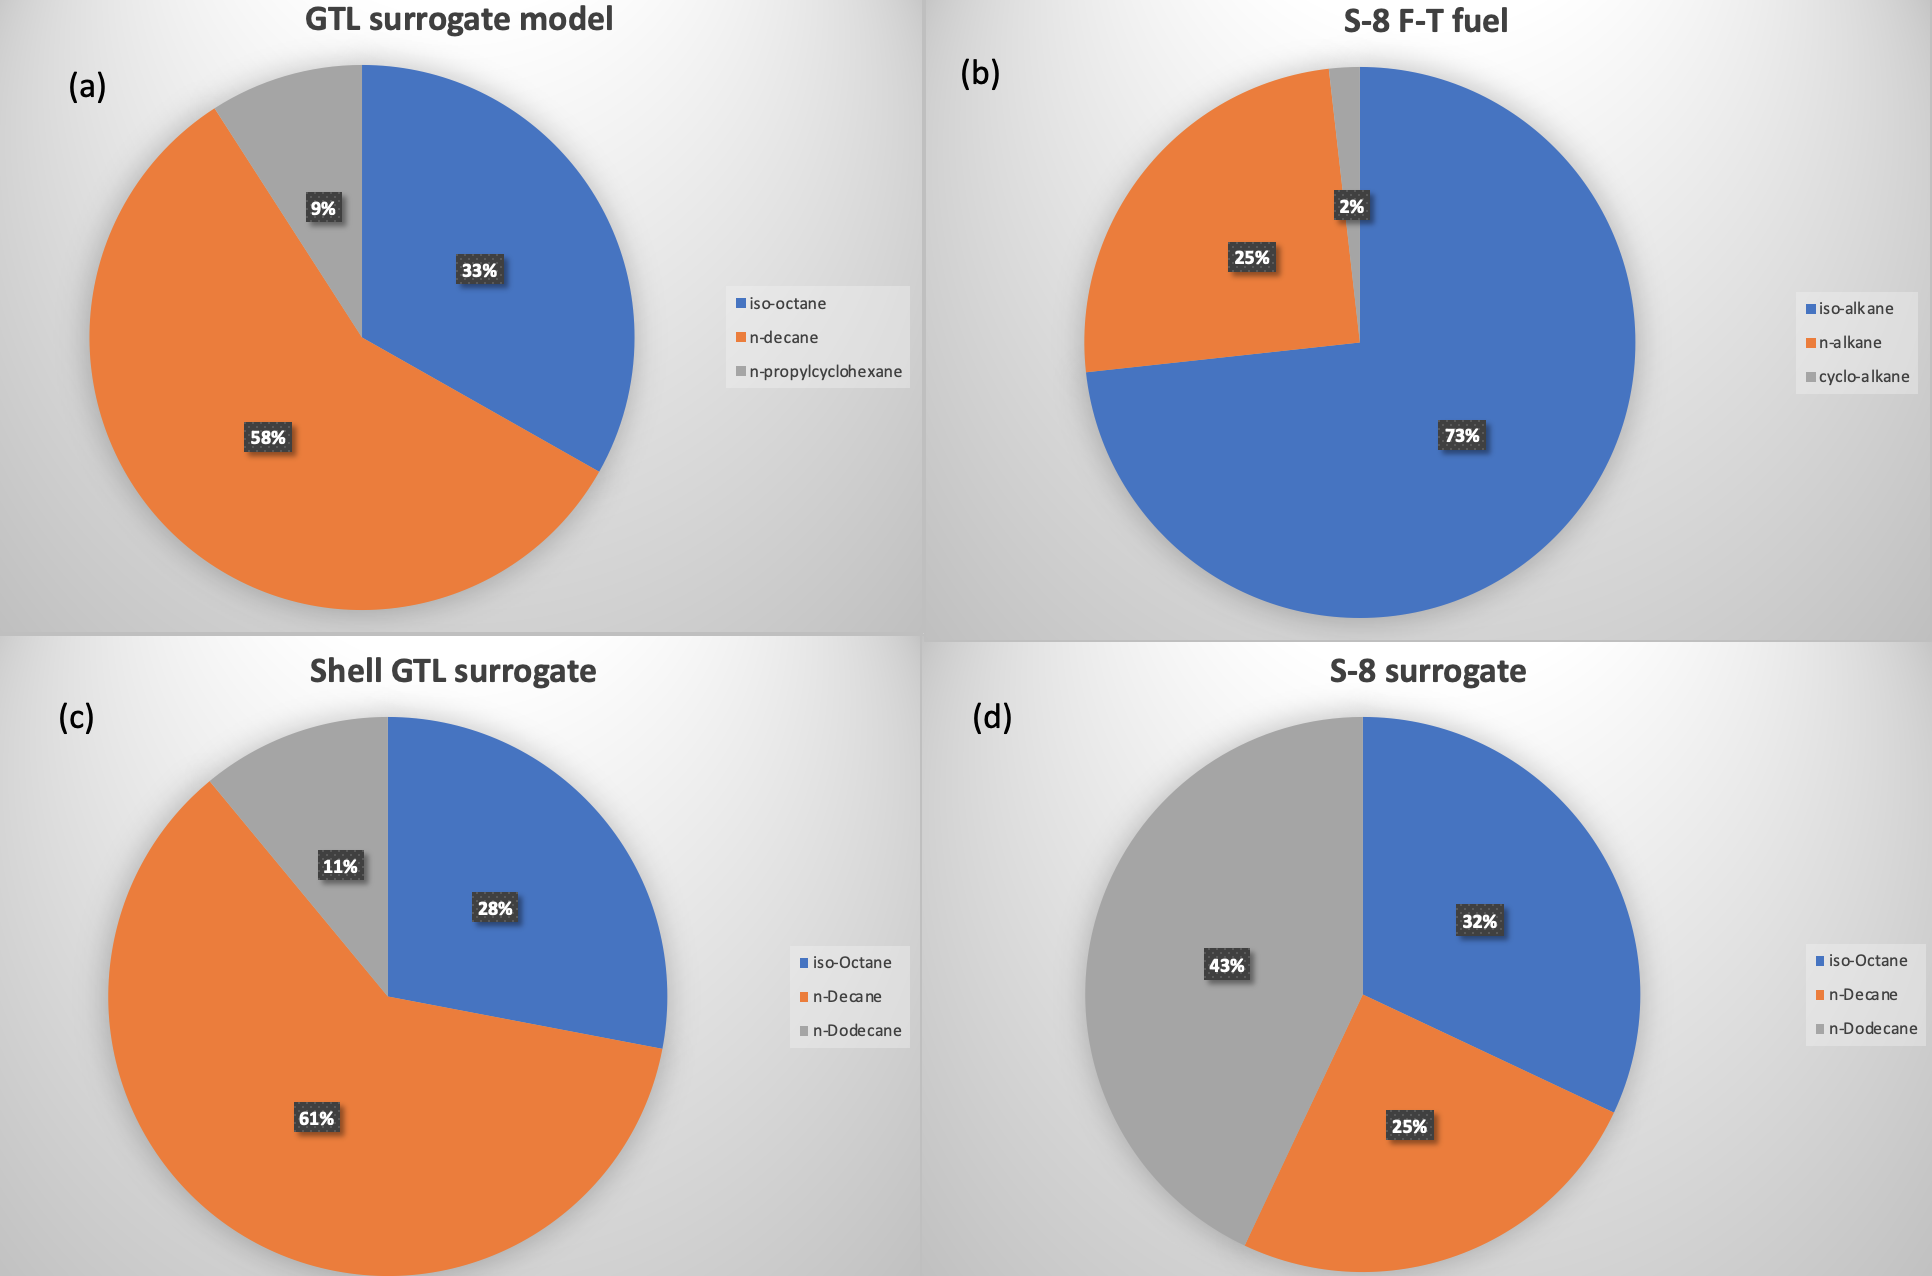
\includegraphics[width=\textwidth, height=\textheight, keepaspectratio]{images/GTL-composition.png}
    \caption{ (a) present work on GTL surrogate model blend \cite{Dagaut2014}, (b) S-8 F-T fuel in \% mol \cite{Naik2011DetailedFuels}, (c) Shell GTL surrogate fuel from Naik et al \cite{Naik2011DetailedFuels}, (d)S-8 surrogate fuel \cite{Moses2008COMPARATIVEREPORT}}
    \label{fig:GTL-composition}
\end{figure}


These methods are based on the mass spectrometry and chromatography analyses of a surrogate composition for primary reference fuel compounds. These surrogates are then used as the guideline to generate chemical kinetic model surrogate fuels that attempt to accurately represent the real fuels under engine-like conditions. The most commonly used blends usually contain paraffins (n-alkanes), olefins, iso-alkanes, naphthenes (cyclic alkanes) and aromatics (arenes). Aromatics are seldom added since it is well known as the primary species responsible for soot formation \cite{RoleOSTI.GOV}. The surrogate models are carefully chosen so they match both the chemical and physical properties like density, viscosity, specific weight, melting and boiling points, flash-points and auto-ignition temperatures. Similarly, the chemical properties such as ignition delay time of the fuel, concentration profiles of species in flow reactors and burning speed are usually the main properties that model generators try to match with the real fuel.

\section{Objective}
Now up until recently, according to the author's knowledge, from literature searches and researchers who have come up with surrogate mixture blends for GTLs, the best practice or framework to building GTL surrogate fuel blended models has been proposed; by either concatenation of the detailed chemical kinetic models of the pure primary reference fuels (PRFs) as given from the spectrometry analysis or a blended mixture of individual species from the onset of the model building process. These two approaches have not yet been tested to see if significant differences exist in the number of species and reactions generated when either of these approaches is used and which approach will closely match both the physical and chemical properties of these fuels as determined through experiments. 

This work focuses solely on the these two aforementioned steps for the automated generation of GTL surrogate fuel chemical kinetic model and its validation with experiments for congruence as well as the effects of each approach on the auto-ignition characteristics of these chemical kinetic blended models. These surrogate models are done with the intention on the best practice for computational modeling as well as completeness to the real surrogate fuel blends that engine designers can utilize in CFD simulations for further design analysis of combustor, fuel injector and other relevant design parameters during the development of new engines that utilize sustainable alternative jet and diesel fuels. 

This thesis is divided into six chapters with the second chapter focused on chemical kinetic mechanisms and the use of RMG in developing a detailed mechanism as well as its algorithm in mechanism generation and thermo-kinetic parameter estimation. The subsequent three separate chapters focus on the detailed kinetic model generation of the PRFs of n-decane, iso-octane and n-propyl-cyclohexane as well as their respective model validation in shock tubes for ignition delay times. The penultimate chapter is focused on the concatenation of the three PRF blends as well as the direct mechanism generation of the GTL fuel surrogate model with its mechanism validation in a shock tube for ignition delay time predictions. 

\chapter{Chemical Kinetic Mechanism Generation}
\section{Overview of Chemical Kinetic Mechanism}
Combustion at its very core, is an interdisciplinary field, that integrates the knowledge of physics of transport and reacting energy levels of species, the chemistry of reactions - rates of reactions (kinetics), fluid dynamics of flow fields, thermodynamics of reacting species based on energy levels both at the classical and statistical (quantum) levels and finally an appreciation of computer software and technology for computational analyses \cite{Curran2019DevelopingCombustion}. As a result of this interdisciplinary nature of the field, significant advances in each sub-discipline is virtually as important in bringing this field together in an age where technology is predominant and an ever increasing need to ensure the survival of the environment and human life, in quest to curb and understand negative effects of combustion, through air pollution from GHG as well as other emissions of harmful pollutants. 

Combustion is applied in almost all forms of daily life, that the understanding of each sub-discipline helps to further the current knowledge and appreciation of how well this field develops. From the very complex process of using internal combustion engines in automobiles, to the rotating shaft of turbines in both stationary gas turbines used in power plants and that of the aero-derivative gas turbines in airplane engines, to the industrial stove and gas burners to fertilizer and chemical processing and even HVAC systems. This plethora of applications has pushed an ever inquisitive solution to make these applications of combustion safer to humans and the environment as well as ensure the life cycle of devices that use these technologies. 

\begin{figure}

\centering
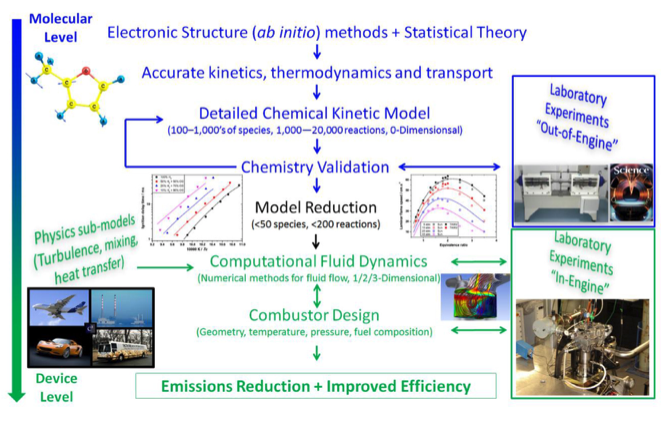
\includegraphics[scale=0.5, keepaspectratio]{images/combustion_schematic.png}
\caption{Schematic Diagram showing the different levels of understanding combustion from theory to application, courtesy of Dr.Kieran Somers \cite{Curran2019DevelopingCombustion}}
\label{fig:combustion_schematic}
\end{figure}

In fig.\ref{fig:combustion_schematic}, an ascending order of how combustion research starts off at :
\begin{enumerate}
        \item The molecular level with the need to understand species electronic structures using statistical theory and ab initio conditions, it includes those calculations of transitions states using quantum methods for reaction rates at intermediates and products used to quantify reacting species. This is the level where quantum methods are dominant and necessary for good estimates at level 2.
        \item Fuel structure and fundamental chemistry of fuel species, which is eventually stored in a database for kinetic, thermodynamic and transport parameters. This database is eventually used as a reference library to build detailed chemical kinetic models of a specific fuel or blends of fuels from elementary reactions using the reference libraries and database, based on the estimates from ab initio conditions of the thermo-kinetic parameters and validated with experimental measurements in homogeneous reactors for ignition-delay times, laminar flame speeds and species concentration profiles as well as rate of production/consumption of species.
        \item The reduction of the chemical kinetic mechanisms, which involves looking at the connection between reacting species and reactions through various methods like Sensitivity Analysis \cite{Rabitz1983SensitivityKinetics},\cite{Turanyi1990SensitivityApplications}, Directed Related Graph Method (DRG) \cite{Lu2005AReduction}, Directed Related Graph with Error Propagation (DRGEP)\cite{Pepiot-Desjardins2008AnMechanisms}, Directed Related Graph with Sensitivity-Analysis (DRGASA)\cite{Sankaran2007StructureFlame}\cite{Zheng2007Experimental13-butadiene}, Directed Related Graph with Error Propagation and Sensitivity Analysis (DRGEPSA) \cite{Niemeyer2010SkeletalAnalysis}, Computational Singular Perturbation \cite{Massias1999AnData}, Rate-Controlled-Reduced-Equilibrium methods (RCCE) \cite{Keck1971Rate-controlledMixtures}, which is done to reduce these kinetic mechanisms to only the core skeletal models of only a few hundred species with unimportant reactions and species removed for easy numerical computation of reactors and engines in CFD analysis that engine designers use.
        \item The last level is involved on practical applications, including policy regulation and efficiency of devices built especially the physical construction and building of these devices like internal combustion engines.
\end{enumerate}  

 So the link from molecular level to macro-level application is so enormous that most researchers typically focus on one or two levels at any given time. Level 2 is the of building detailed chemical kinetic models and exemplifies what this work is framed on for the purpose of GTL fuel surrogates. While, there will be mentions of level 1 during the course of the next chapters, level 2 entails the bulk of this thesis. 
 
 
\section{What is a Chemical Kinetic Mechanism ?}
 A chemical kinetic mechanism is numerical model that accurately contains the detailed elementary reactions of reacting species, thermodynamic estimates, associated rate constants with collider species, transport species at the specified reactor conditions of temperature, pressure and mole ratio \cite{Curran2019DevelopingCombustion}. This chemical kinetic mechanism can be very useful in describing reactions that are well known such as that of methane with oxygen described by the global reaction 
 
     \reaction{CH4 + 2O2 \longrightarrow CO2 + 2H2O}
 
 
 which really looks like a one-step reaction, however, contains about 200 elementary reactions and about 30 different species at a wide range of pressures and temperatures. Each elementary reaction describes the reactant and product species as well as the rate constant in both forward and reverse directions for a reversible reaction,
 
     \reaction{A\underset{k_r}{\stackrel{k_f}{\rightleftharpoons}}B}
  
 the forward rate constant $\ce{k_f}$ is often written as \ce{k_f[A]} while that of the reverse rate constant $\ce{k_r}$ is often written as \ce{k_r[B]}. This reaction rate constant is defined by the Arrhenius form defined as
 \begin{equation}
    k_f = A\times e^-{\frac{E_a}{RT}}
 \end{equation}
 \[\text{or that of the modified Arrhenius}\], 
 \begin{equation}
    k_f=A\times T^{\alpha}\times e^-{\frac{E_a}{RT}}
 \end{equation}
  At equilibrium, the forward and reverse rate constants are equal, thus
  \begin{equation}
  K_{eq}=K_c
  \end{equation}
  \[\text{also that} \]
  \begin{equation}
      K_{eq}=-\frac{\Delta G_r}{RT} 
  \end{equation}
  \[\text{and that}\]
  \begin{equation}
     K_c=\frac{k_f}{k_r}
  \end{equation}
  Then, at chemical equilibrium, 
  \begin{equation}
     K_{eq}=K_c=\frac{k_f}{k_r}
     \therefore K_{eq} = \frac{k_f}{k_r}
  \end{equation}
  
  and knowing that 
  \begin{equation}
    \Delta G_r = \Delta H_R -T\Delta S_R  
  \end{equation}
Where, $\Delta G_r$ is the Gibbs Free Energy of the reaction - indicating the energy available to do non-boundary (PV) work in a thermodynamically closed system at constant temperature and pressure and $\Delta H_R$ is the enthalpy of the reaction and $\Delta S_R$ is the entropy of the reaction. Thus, for reacting species, since the thermo-kinetic parameters of the forward rate constant is known, the corresponding reverse rate constant can be calculated from the equilibrium constant as a thermodynamic equilibrium is established. A chemical kinetic mechanism contains the thermo-kinetic parameters for the forward rate constants of elementary reactions at defined temperatures and pressures as well as the thermodynamic estimates and third body colliders. For flammability characteristics, the transport properties are also included in the mechanism.
 
 \section{Improvements in Chemical Kinetic Mechanisms}
 As a result of the complex reactions and reaction pathways involved in getting all possible elementary reactions and rate constants that describe many applicable reactions in combustion, the chemical kinetic modeling community has made significant improvements in the last three decades, with the development of various mechanisms aided with reaction pathways generated through automated computation, mechanisms such as the GRI-Mech\cite{Frenklach1995GRI-Mech---AnGRI-95/0058}\cite{BowmanGRI-Mech2.11}\cite{SmithGRI-Mech3.0} that was used to predict \ce{NOx} predictions and emissions of natural gas (methane),  Lawrence Livermore National Labs (LLNL) models of n-heptane and iso-octane as primary reference fuels of gasoline surrogates \cite{Curran1998AOxidation}\cite{Curran2002AOxidation}. As a result of the advances in computing technology, more complex models with more species and reactions have been built as seen in fig.\ref{fig:model_history} with carbon chains to \ce{C16} and \ce{C20}\cite{Westbrook2009AN-hexadecane}\cite{Sarathy2011ComprehensiveC20} and even oxygenated fuels \cite{Fischer2000TheReactors} as well as surrogate fuel models \cite{Mehl2011AnModelingb}. Recent strides have also been made towards the generation of jet fuel surrogate models \cite{Gokulakrishnan2008IgnitionFuel} \cite{Dooley2010AProperties}\cite{Mze-Ahmed2010KineticsStudy}\cite{Wang2012}\cite{Dagaut2014}\cite{Dagaut2014CombustionModeling}\cite{Narayanaswamy2016ASurrogates}\cite{Dagaut2016ExperimentalSurrogates}\cite{Singh2011ExperimentalFlames}. 
 
 \begin{figure}[hbp]
 \hspace*{-2cm}
     \centering
     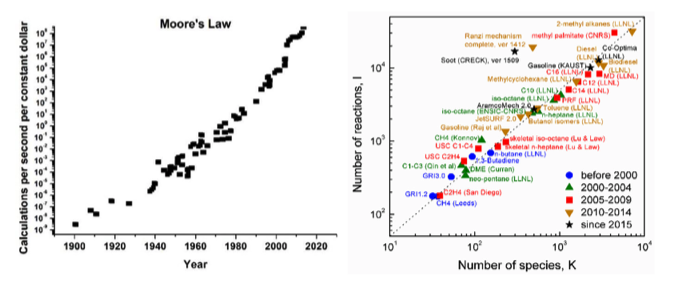
\includegraphics[scale=0.75,keepaspectratio]{images/model_history.png}
     \caption{Illustration of the correlation between computing power and mechanism size. Right hand side courtesy of Prof. Tianfeng Lu \cite{Curran2019DevelopingCombustion}}
     \label{fig:model_history}
 \end{figure}
 
 
 Most published kinetic models are validated with some uncertainty or error based on the estimates used, moreover since there exists no central database with which species estimation is benchmarked against save some experimental data or previous model, it is pertinent that a database be created not just for the estimation but also for the model generation of primary reference fuels for surrogates as well as comprehensive, detailed models of individual fuels validated against experiments such as ignition-delay times, laminar flame speeds and species concentration. Such database can be made into a library with easy access to determine where each model originates as well as how to construct more complex fuels based on the core mechanism of the \ce{C_0-C_4} chemistry. This quest for both a database library and automated model generation has birthed the use of more robust chemical kinetic mechanism software. 
 
 \section{Auotmated Chemical Kinetic Mechanism}
 The correlation between chemical kinetic mechanism and computing power has grown significantly over the years as seen in fig.\ref{fig:model_history} that it is almost impossible to attempt to build models without the aid the these numerical networks. As computing technology as improved as well as optimization of numerical methods, more models have been generated using automated software as well as interactive algorithms for the simulation of chemical mechanisms. The rise of Reaction Design's CHEMKIN suite originally developed by Sandia National Laboratories in the 1980's and now owned by ANSYS \cite{ANSYSCHEMKIN-PRO}, EXGAS \cite{Warth2000ComputerOxidation}, OPENSMOKE++\cite{Cuoci2015OpenSMOKE++:Mechanisms}\cite{Cuoci2013NumericalMethod}\cite{Stagni2014LumpingCoupling},LOGE-soft\cite{LOGESOFT}, Cantera\cite{cantera}, FlameMaster\cite{Pitsch1990FlameMasterCalculations}, CosiLab\cite{CosilabLaboratory}, CMCL Innovations kinetics\cite{ComputationalBuilder}, DETCHEM\cite{Deutschmann2019DETCHEMEd.},Chemical WorkBench\cite{Kintechlab:ChemicalWorkBench}, RMG\cite{Gao2016ReactionMechanisms}\cite{Allen2012AutomaticCoefficients}\cite{Magoon2013DesignGeneration}. These computer softwares are capable of generating chemical kinetic mechanism and validation of those mechanism with respect to some experimental measurement. There are four main capabilities needed for automatic chemical kinetic mechanism generators to possess to be able to be robust in the simulation of chemical species. They are:
 \begin{enumerate}
     \item A unique way to identify and represent chemical species correctly
     \item A method to determine what and how reactions can occur between chemically reacting species
     \item A means of getting good thermodynamic and kinetic estimates of parameters
     \item A criteria for inclusion or exclusion of species in the reaction model
 \end{enumerate}
     
 These numerical models continuously solve differential equations of the chemical reacting species based on some initial condition usually given or derived from experiments or boundary condition. The integration of these species is done by applying conservation laws of energy, mass, species and linear momentum for flame simulations within a given step size. As the integration continues, the time steps are adjusted for the next quantity estimating the temperature, pressure, velocity, species-concentration or mole fractions. The schemes used by most numerical solvers typically depend on the physical system being modeled, geometry, step-size and convergence criteria imposed. At any given time, if the time-step changes more faster than the solver scheme then it is bound to either fail or give incorrect approximations. As a result, most solvers are constrained to usually do uniform step-sizes as well as imposing a constant parameter to enable more efficient computation. 
 
 This work uses the reaction mechanism generator (RMG)\cite{Gao2016ReactionMechanisms}\cite{Allen2012AutomaticCoefficients}\cite{Magoon2013DesignGeneration} to construct three-component primary reference fuel (PRF) surrogate as a representation of GTL fuels. Each PRF consists of a detailed kinetic model with validations against experimental data. More emphasis is now laid on how RMG generates its models and the steps taken to build each PRF of n-decane, iso-octane and n-propyl-cyclohexane. 
 
 \newpage
 
 \section{Chemical Kinetic Mechanism Generation using Reaction Mechanism Generator (RMG)}
 \subsection{How RMG Works}
 RMG is an open-source software package that was developed at the Green Group at MIT to assist researchers and industry in the physical and chemical modeling of chemical reaction processes of elementary reactions. It is a Python based code of over 60,000 lines that also has the ability to calculate quantum estimates of species as well as at transition states.In addition, RMG has the unique capability of estimating transport properties for flamelet models and flammability analyses as well as solvation properties for liquid-phase species and automatically computes pressure-dependent rate constants and pressure-dependent rate networks for reaction flux analysis.
 
 RMG works on the framework of the general understanding of underlying reaction of elementary reactions and how they react. It employs the use of known chemistry methods stored in its library database from other chemical kinetic mechanisms along with its own unique property estimation methods to generate detailed chemical kinetic mechanisms. It relies primarily on two key principles: graph and tree structures to represent chemical species and represent both thermodynamic and kinetic parameters respectively. 
 
 Models are generated using a rate-based algorithm, which tracks the flux of species and excludes species based on the reaction flux criteria. RMG can generate mechanisms for species containing carbon, hydrogen, oxygen, sulphur and nitrogen \ce{C, H_2, O_2, S, N_2}.In order to construct a mechanism, an interactive script is first written for the specific set of species to be reacted as well as the reactor conditions for the reaction at initial conditions. Such conditions typically include temperature, pressure, species concentrations. RMG then takes the initial starting species and reacts all the species in all possible ways based on its own reaction families and then does a time integration of the model. 
 
 RMG tracks the rate of production of species as well as reactions at the edge (outside the initial starting species). As the reactions occur, the rate of production of new species and reactions outside the initial starting species grows with significance, the new reactions and species produced from further reaction is then added to the core of the initial starting species and the model grows bigger in size. As the new core species are then reacted with all other new species in the core thus, generating much species and reactions.As the time integration restarts, the list of edge species are tracked to determine which species will be added again to the core. This process continues until all the significant species are added to the core. A significant rate can be specified by the user, by using the following definition: 
 \begin{equation}
     R_i=\frac{dC_i}{dt}
 \end{equation}
 When the flux (rate of production of species) in the edge is greater than that of the characteristic species, it is moved to the core. The reaction system characteristic rate is the sum of the all core species rates, defined as:
 \begin{equation}
     R_{char}=\sqrt{\sum_j {R_{j}^2}} \hspace{1cm} \text{species j $\epsilon$ core}
 \end{equation}

 
 \begin{figure}[htp]
     \centering
     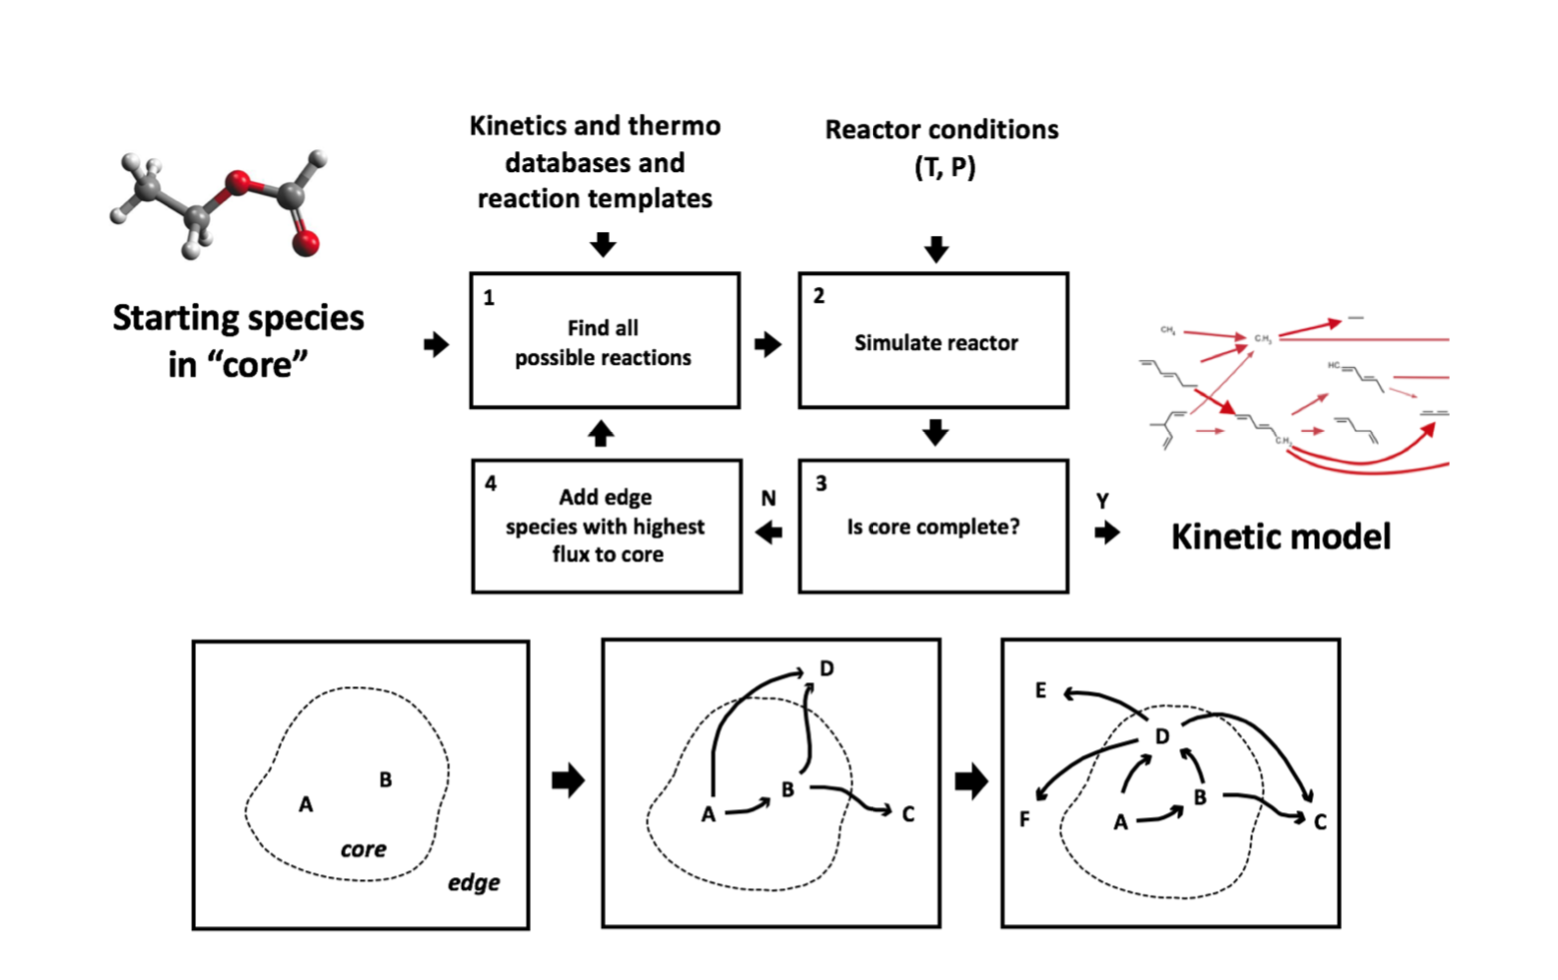
\includegraphics[scale=0.4,keepaspectratio]{images/rmg_core_build.png}
     \caption{RMG Rate-based Model Englarging Algorithm Schematic \cite{Susnow1997Rate-BasedSystems}\cite{Gao2016ReactionMechanisms}}
     \label{fig:rmg_core_build}
 \end{figure}
 
 RMG utilizes a functional group based algorithm to work with species and reactions. It is applied in such a way that each reactions family is defined by a set of templates that match functional groups as they go from reactants to products\cite{Gao2016ReactionMechanisms}. Chemical graph theory is applied for representing molecules as well as functional group substructures, with vertices indicating atoms while edges are used to indicate bonds.
 
 \subsection{RMG Thermodynamic Estimation}
 Species thermochemistry is estimated using Benson group additivity methods \cite{Benson1958AdditivityProperties}\cite{Benson:452788}for thermochemical parameters, such as enthalpy $\Delta H_f^{\circ}$, entropy $S^{\circ}$ and heat capacities $c_p$. For free radical, the hydrogen bond increment (HBI) method of Lay et al is applied \cite{Lay1995HydrogenSpecies}. RMG utilizes hierarchical trees to organize functional groups for ease of group identification. Trees structures are organized in such a way that the general functional groups are placed at the top nodes, then more specific functional groups are placed in the successive lower nodes.  Before thermodynamic estimates are computed, resonance structures of those species are run and obtained including non-straight chain (aromatic) structures of the species. The algorithm then checks for the presence of radicals in any of the resonance structures, which if present the HBI correction is applied, before proceeding to check for the contribution of the enthalpies, entropies and heat capacities of the saturated species. .
 \begin{figure}[ht]
     \centering
     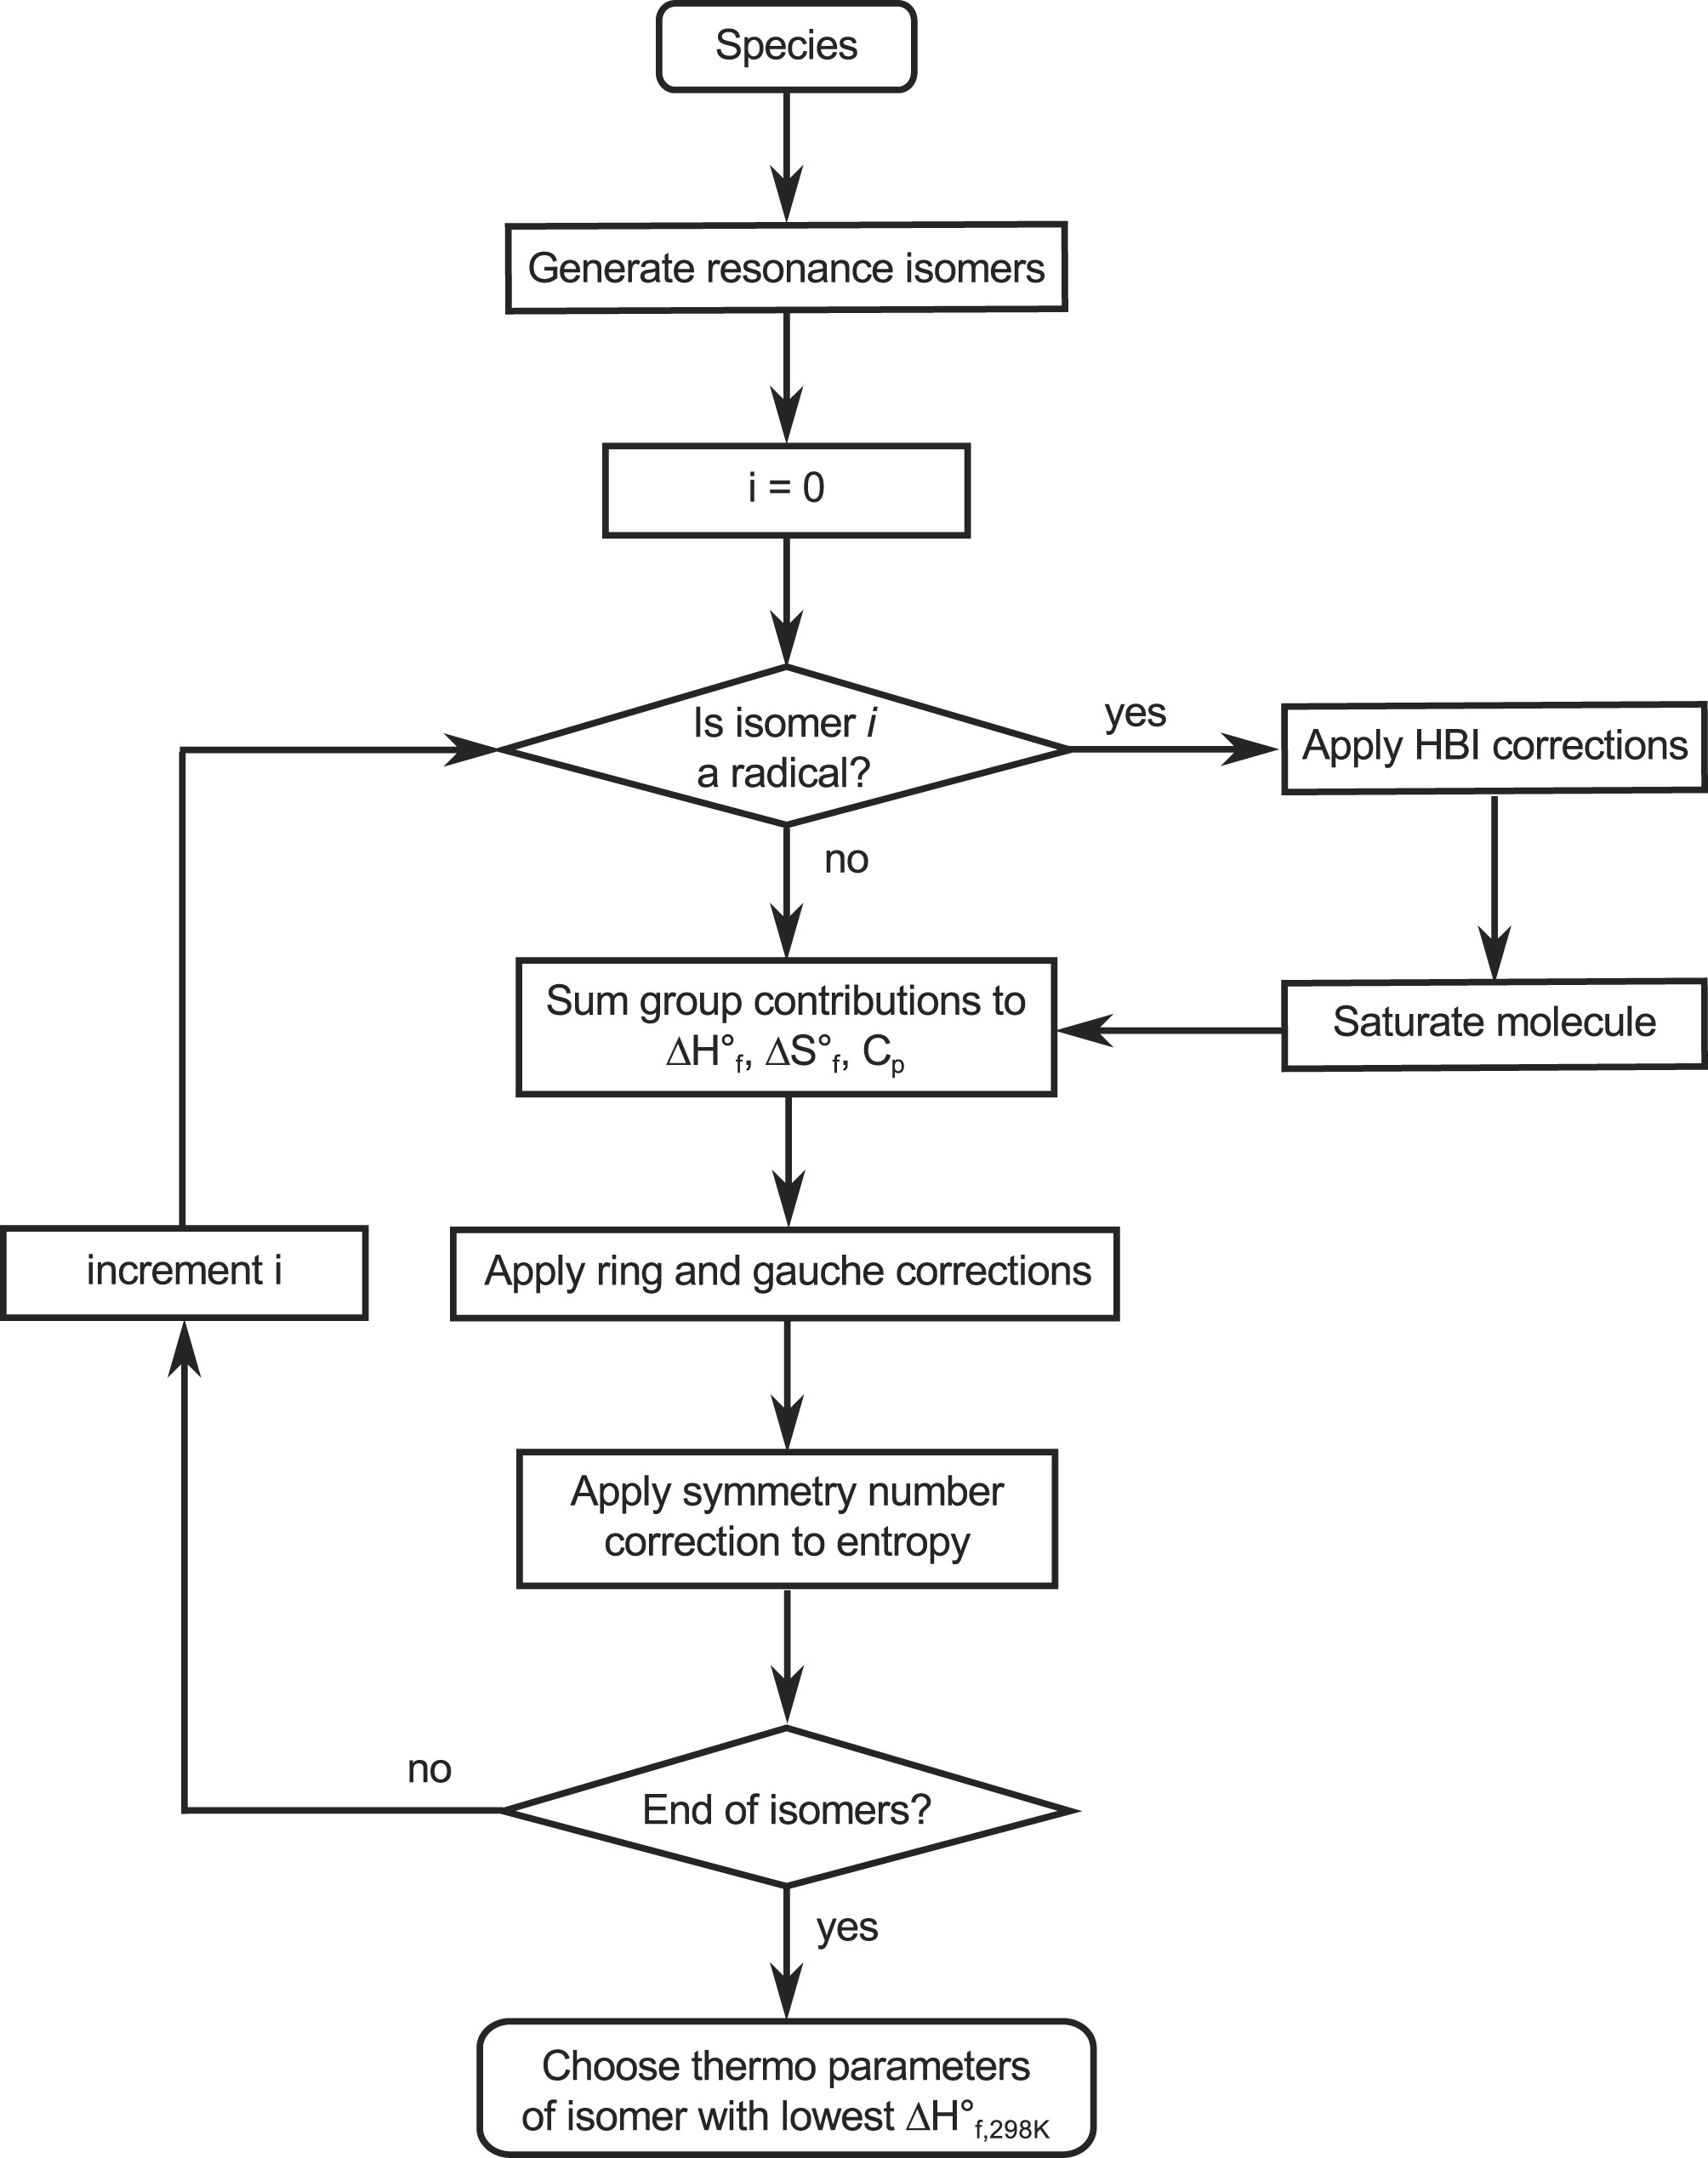
\includegraphics[scale=0.85]{images/tree-structure.jpg}
     \caption{RMG group-additivity thermodynamic parameter estimation algorithm \cite{Gao2016ReactionMechanisms}}
     \label{fig:tree}
 \end{figure}
 This entire process is done for before symmetry checks are applied to the total symmetry number of $\sigma$ bond correction at the entropy of formation.
\begin{equation}
    S^{\circ}=S_{GA}^{\circ}-R\ln\sigma
\end{equation} 
where, $S^{\circ}$ represents the standard corrected entropy of formation at 298K and $S_{GA}^{\circ}$ represents the group additivity standard entropy of formation at 298K, R is the gas constant. In fig.\ref{fig:tree} shows the entire algorithm followed for group-additivity thermodynamic estimation
 
 
 
 
 \subsection{RMG Kinetic Estimation}
 RMG is able to generate elementary reactions based on its library database of 45 reaction families of species. Each reaction family has a series of templates by which the reactive sites are identified as well as which reaction recipe to follow in order for bond connectivity to change as reactions proceed from reactants to products. Another set of hierarchical tree is used for rate estimates, assigning kinetics between reaction sites based on the closest matching functional group. The list of RMG reaction families are shown in the appendix.
%  
 
 
 
 
 In RMG, the forward rate constants are well defined based on thermodynamic parameters in its library database. Since the equilibrium constant $K_{eq}$ is also known again based on the thermodynamic estimates, the reverse rate is then given as \begin{equation}
     k_r=\frac{k_f}{K_{eq}}
 \end{equation}


\subsection{Seed Mechanisms}
Seed mechanisms are reaction libraries of other kinetic models that are automatically added to the model generation in RMG. The user starts off using a seed mechanism so as to guide RMG in the specific species, that must be included in the core of the model as well as the rates used in the quantification of these species rather than RMG's own group-additivity methods. This practice is done when a specific species or set of rates must be included in the mechanism. For the GTL PRFs, multiple seed mechanisms were used in order to reproduce the bulk of the species found in the literature and controls the auto-ignition properties of the fuel.


\subsection{Reactors with Pressure Dependence}
Unimolecular reactions are reactions that occur alone as only one reactant is present. These reactions in the process of going from reactants to products, require sufficient energy to overcome the energy barrier. Since these reactions can occur via isomerization such as \reaction{A\rightleftharpoons B} as well as that of dissociation or association reactions where \reaction{A\rightleftharpoons B + C} For gas-phase reactions to occur, it must be due to collisions as known in the Kinetic Theory of Gases. Thus, there must be a collider gas or an increase in the pressure of the system. If the sole reactant is then excited to a higher energy state, it thus possesses sufficient energy to overcome the activation energy barrier. If that activated species is excited it is then denoted as \reaction{A^* \rightleftharpoons B^*} and \reaction{A^* \rightleftharpoons B + C} The activated species can thus be activated in one of the following ways:
\begin{enumerate}
    \item Chemical activation such that $A^*$ is the product of the association reaction \reaction{B + C \rightleftharpoons A^*}
    \item Thermal activation which occurs when a collider species usually inert transfers energy to the reacting species through bimolecular collision \reaction{A + M \rightleftharpoons A^* + M} where M is the inert gas
    \item Photoactivation where A* is the product of a photon absorption
    \reaction{A + h\nu \longrightarrow A^*}
\end{enumerate}

Once a species has been activated, multiple reactions then occur often competing between themselves - between isomerizations and bimolecular reactions and as they attain collisional stabilization or thermal deactivation, they form a network of unimolecular reactions. The dominant pathway depends on the relative rates of collision and the reactions, which is now a function of temperature and pressure. At higher pressures, the collision rate is fast and activated species tend to attain thermal deactivation (collisional stabilization) before further reactions occur, usually referred to as the high-pressure limit. Similarly, at lower pressures, the collision rates are low and more reactions of the species occur between dissociations and isomerizations  before collisional stabilization is attained. The region at which pressure-dependence begins to affect reactions varies with temperature and molecular size\cite{Wong2003TemperatureLimit} as seen in fig.\ref{fig:pdep}.

\begin{figure}[t]
    \centering
    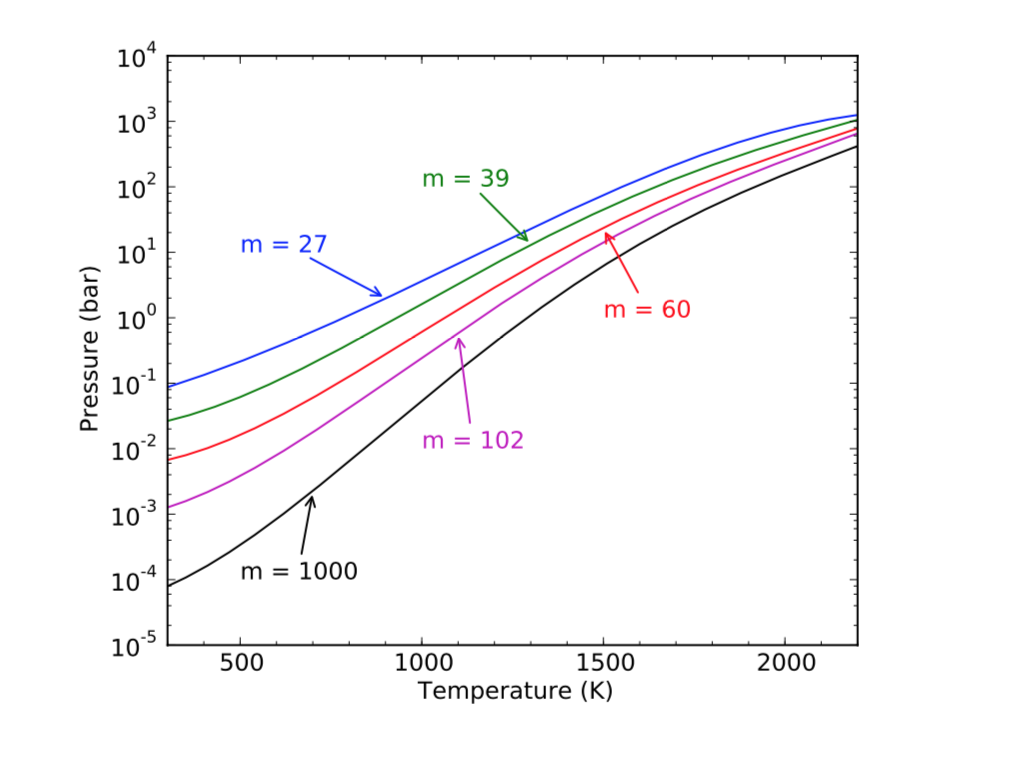
\includegraphics[scale=0.75, keepaspectratio]{images/pdep_limit.png}
    \caption{Plot of the switchover pressure - indicating the onset of pressure dependence - as a function of temperature and molecular size. The value $m\equiv N_{vib}+\frac{1}{2}N_{rot}$ represents a count of the internal degrees of freedom. Over a wide variety of conditions of practical interest, even very large molecules exhibit significant pressure dependence. \cite{Wong2003TemperatureLimit}}
    \label{fig:pdep}
\end{figure}
For the bulk of this work on all the PRFS of n-decane, iso-octane and n-propyl-cyclohexane, pressure dependence based on the guide of \cite{Wong2003TemperatureLimit} and fig.\ref{fig:pdep} was used to certify why pressure dependent models were necessary in building the GTL surrogates.

\vspace{1.5cm}

\subsection{Rate-based Algorithm and Filtering Reactions}
RMG makes use of the algorithm of Susnow et al \cite{Susnow1997Rate-BasedSystems} to decide which model species and reactions are included in the the core of the mechanism. The Algorithm as shown in the illustration of fig.\ref{fig:rmg_modelflux} with a grpahic illustration in fig.\ref{fig:rate-schematic}shows how the model generation process occurs and the decision tree for model move to core criteria. Since each model starts off with only user defined set of initial conditions as well as convergence criteria (termination condition for model generation to stop), the model termination can be a set of conditions such terminationtime, species conversion and terminationrateratio.
\begin{figure}[ht]
    \centering
    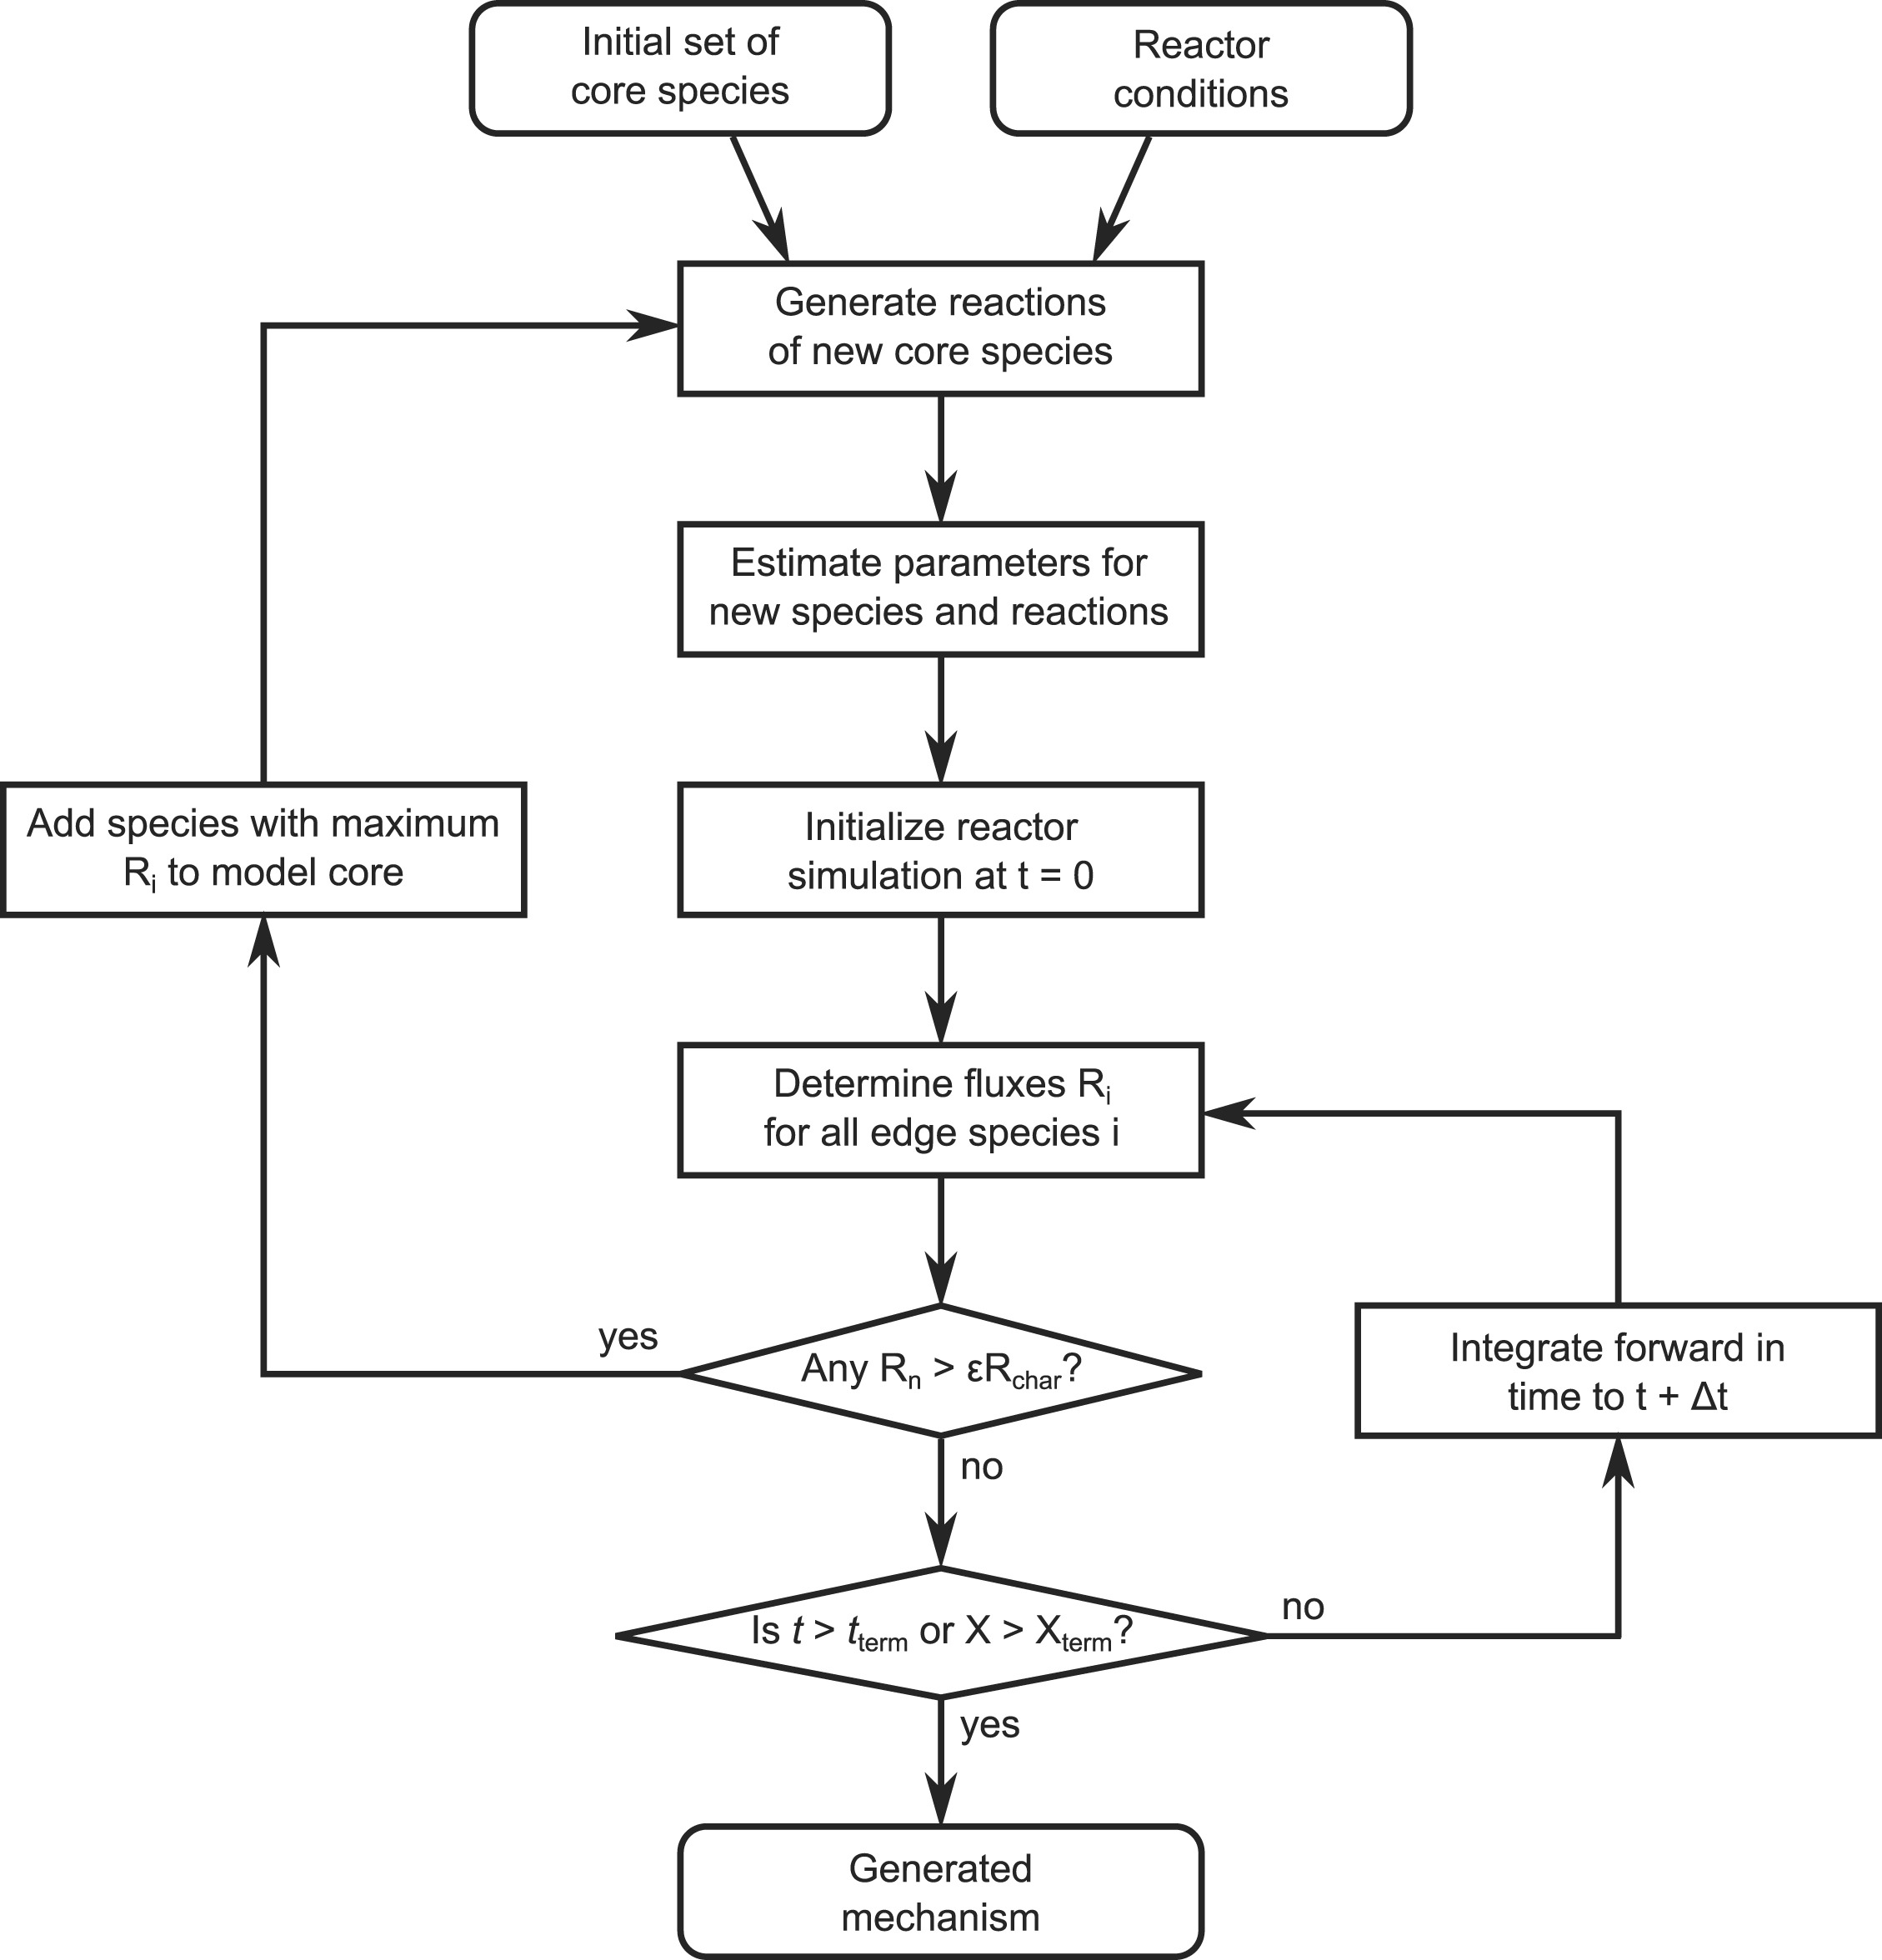
\includegraphics{images/rmg_model_flux.jpg}
    \caption{Flowchart of the Susnow et al\cite{Susnow1997Rate-BasedSystems} model rate algorithm as implemented in RMG}
    \label{fig:rmg_modelflux}
\end{figure}

Since RMG typically generates models at well defined and set temperature and pressure reactors, the need to generate models that span a wide range of temperatures and pressures is important. Rather than set a fixed constant temperature and pressure condition for reactors, RMG has a unique capability of doing a range based reactor. This means that RMG takes in various reactor conditions of temperature, pressure and species concentrations, using a weighted stochastic grid sampling algorithm, RMG samples the space of the range reactor conditions given based on the previous run conditions evaluated at the combination of the temperature pressure concentration pair. Each iteration is a grid of points spanning the reactor range where the grid has $20^N$ points and N is the number of dimensions.The grid values are normalized to one and a grid is chosen with a probability that is equal to the normalized objective function. A random step of maximum length is taken at a $\sqrt{2}/2$ times the distance between each grid point to the point of interest where the sampling starts. With this algorithm, RMG is able to then generate models at reactor range conditions and thereby reduce the computational cost of running at various points. 

\begin{figure}[ht]
    \centering
    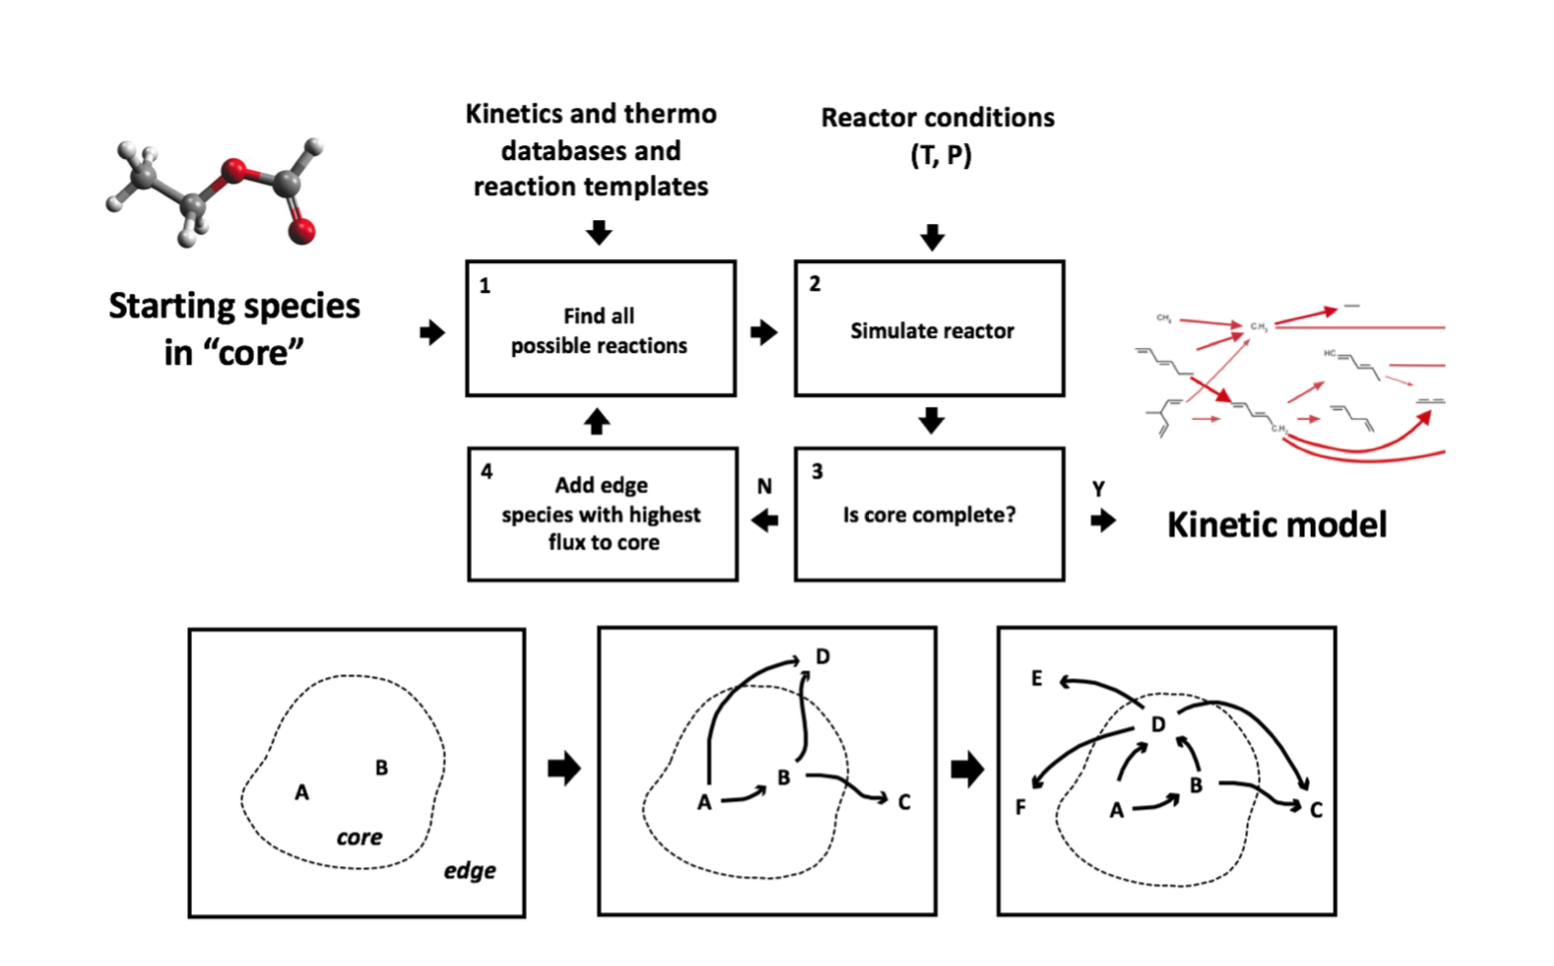
\includegraphics[scale=0.45,keepaspectratio]{images/rate-schematic.png}
    \caption{Schematic of the rate-based enlarging algorithm as described by Susnow et al\cite{Susnow1997Rate-BasedSystems} and illustration from RMG team\cite{Gao2016ReactionMechanisms}}
    \label{fig:rate-schematic}
\end{figure}


This range reactor model was applied on all PRF models of the GTL fuel surrogate (n-decane, iso-octane and propyl-cyclohexane) as well as the mix of all species of the PRFs in the starting input file.


\newpage

\section{Model Generation of PRFs in RMG}

Since RMG has all the capabilites needed to fully generate a detailed chemical kinetic mechanism, the PRFs of this GTL fuel blend was constructed using the aforementioned strategies outlined in Table \ref{tab:PRF_table}. 


\begin{table}[ht]
\arrayrulecolor[HTML]{DB5800}
\caption{Summary of the RMG input parameters in the database block for the model generation of PRFs: n-decane, iso-octane, n-propyl-cyclohexane and the GTL blend with input species}
\centering
\begin{adjustbox}{width=1\textwidth}
\small
\begin{tabular}{ p{5cm} p{5cm} p{5cm} p{5cm} p{5cm} }
    \hline
    \rowcolor{lightgray} \multicolumn{5}{|c|}{RMG PRF Input File Options} \\
    \hline
    Model Syntax  & n-decane & iso-octane & n-propyl-cyclohexane & GTL model blend with all PRF species added \\
    \hline
    thermoLibraries used \\
    - & BurkeH2O2 & BurkeH2O2 & BurkeH2O2 & BurkeH2O2 \\
    - & Klippenstein\textunderscore Glarborg2016 & Klippenstein\textunderscore Glarborg2016 & Klippenstein\textunderscore Glarborg2016 & Klippenstein\textunderscore Glarborg2016 \\
    - & CurranPentane & CurranPentane & CurranPentane & CurranPentane \\
    - & FFCM1(-) & FFCM1(-) & FFCM1(-) & FFCM1(-) \\
    - & primaryThermoLibrary & primaryThermoLibrary & JetSurF2.0 & JetSurF2.0 \\
    - & thermo\textunderscore DFT\textunderscore CCSDTF12\textunderscore BAC &  thermo\textunderscore DFT\textunderscore CCSDTF12\textunderscore BAC & primaryThermoLibrary & primaryThermoLibrary \\
    - & DFT\textunderscore QCI\textunderscore thermo & DFT\textunderscore QCI\textunderscore thermo & thermo\textunderscore DFT\textunderscore CCSDTF12\textunderscore BAC & thermo\textunderscore DFT\textunderscore CCSDTF12\textunderscore BAC \\
    - & CBS\textunderscore QB3\textunderscore 1dHR & CBS\textunderscore QB3\textunderscore 1dHR & DFT\textunderscore QCI\textunderscore thermo & DFT\textunderscore QCI\textunderscore thermo \\
    - & - & - & CBS\textunderscore QB3\textunderscore 1dHR & CBS\textunderscore QB3\textunderscore 1dHR \\
    \hline
    reactionLibraries used \\
    - & CurranPentane & CurranPentane & violator\textunderscore fixes\textunderscore 500-1500K & JetSurF2.0 \\
    - & FFCM1(-) & FFCM1(-) & JetSurF2.0 & FFCM1(-) \\
    - & combustion\textunderscore core/version5 & combustion\textunderscore core/version5 & CurranPentane & combustion\textunderscore core/version5 \\
    - & - & - & FFCM1(-) & - \\
    - & - & - & combustion\textunderscore core/version5 & - \\
    \hline
    seedMechanisms \\
    - & BurkeH2O2inN2 & BurkeH2O2inN2 & BurkeH2O2inN2 & BurkeH2O2inN2 \\
    - & Klippenstein\textunderscore Glarborg2016 & BurkeH2O2inArHe & Klippenstein\textunderscore Glarborg2016 & Klippenstein\textunderscore Glarborg2016 \\
    - & \ce{C2H4+O\textunderscore Klipp2017} & \ce{C2H4+O\textunderscore Klipp2017} & \ce{C2H4+O\textunderscore Klipp2017} & \ce{C2H4+O\textunderscore Klipp2017} \\
    - & - & Klippenstein\textunderscore Glarborg2016 & - & - \\
    \hline 
    kineticDepositories used \\
    - & training & training & training & training \\
    \hline
    kineticsFamilies used\\
    - & default & default & default & default \\
    \hline
    kineticsEstimator used\\
     - & rate rules & rate rules & rate rules & rate rules \\
    \hline
    \end{tabular}
    \end{adjustbox}
    
    \label{tab:PRF_table1}
    
\end{table}

The additional set of options in RMG, which aided in the construction of the PRFs as well as the GTL mixture blend was done to enable computational efficiency as well as proximity to the real GTL fuel blend as described in \cite{Dagaut2014}.


\begin{table}
\arrayrulecolor[HTML]{DB5800}
\caption{Summary of the RMG input parameters in the simple reactor 1-2 block for the model generation of PRFs: n-decane, iso-octane, n-propyl-cyclohexane and the GTL blend with input species}
\centering
\begin{adjustbox}{width=1\textwidth}
\begin{tabular}{ p{5cm} p{5cm} p{5cm} p{5cm} p{6cm} }
    \hline
    \rowcolor{lightgray} \multicolumn{5}{|c|}{RMG PRF Input File Options} \\
    \hline
    Model Syntax  & n-decane & iso-octane & n-propyl-cyclohexane & GTL model blend with all PRF species added \\
    \hline
    SimpleReactor 1 Conditions \\ 
    \hline
    temperature range & 550K - 1500K & 550K - 1500K & 550K - 1500K & 550K - 1500K \\
    pressure range & 1 bar - 40 bar & 1 bar - 40 bar & 550K - 1500K & 550K - 1500K \\
    nSims & 10 & 30 & 30 & 40 \\
    initial Mole Fractions  \\
    Fuel & \[\frac{0.000983928}{2} - 0.000983928\times 2\] & \[\frac{0.0165224}{2} - 0.0165224\times 2\]   & \[\frac{0.015748}{2} - 0.015748\times 2\] &  \begin{tabular}{ c }
         n\ce{C_{10}H_{22}}: $\frac{0.000577}{2} - 0.000577\times 2$  \\
         i\ce{C_8H_{18}}:   $\frac{0.000332}{2} - 0.000332\times 2$ \\
         n\ce{C_9H_{18}}: $\frac{0.000091}{2} - 0.000091\times 2$ \\
                                                            \end{tabular}\\ 
    \ce{N2} & 0.983765 &  0.776947 & 0.787402 & 0.787402 \\
    \ce{O2} & 0.0152509 & 0.20653 & 0.19685 & 0.19685 \\
    terminationConversion & - & - & - & \begin{tabular}{ c } 
          n\ce{C_{10}H_{22}}: 0.90\\
          i\ce{C_8H_{18}}: 0.90 \\
          n\ce{C_9H_{18}}: 0.99 \\
    \end{tabular}\\
    terminationTime & 1.0 s & 40.0 s & 40.0 s & 40.0 s \\
    terminationRateRatio & 0.01 & 0.01 & 0.05 & 0.01 \\
    \hline
     SimpleReactor 2 Conditions \\
     \hline
    temperature range & 550K - 800K & 550K - 800K & 550K - 800K & 550K - 800K \\
    pressure range  & 1 bar - 40 bar & 1 bar - 40 bar & 1 bar - 40 bar & 1 bar - 40 bar \\
    nSims & 10 & 60 & 60 & 60 \\
     initial Mole Fractions & \[\frac{0.000983928}{2} - 0.000983928\times 2\]  & \[\frac{0.0165224}{2} - 0.0165224\times 2\] & \[\frac{0.015748}{2} - 0.015748\times 2\]  & \begin{tabular}{ c }
         n\ce{C_{10}H_{22}}: $\frac{0.000577}{2} - 0.000577\times 2$  \\
         i\ce{C_8H_{18}}:   $\frac{0.000332}{2} - 0.000332\times 2$ \\
         n\ce{C_9H_{18}}: $\frac{0.000091}{2} - 0.000091\times 2$ \\
    \end{tabular}\\  
    \ce{N2} & 0.983765 &  0.776947 & 0.787402 & 0.787402 \\
    \ce{O2} & 0.0152509 & 0.20653 & 0.19685 & 0.19685 \\
    terminationConversion & - & - & - & \begin{tabular}{ c }
          n\ce{C_{10}H_{22}}: 0.99\\
          i\ce{C_8H_{18}}: 0.99 \\
          n\ce{C_9H_{18}}: 0.99 \\
    \end{tabular}\\
    terminationTime & 1.0 s & 40.0 s & 40.0 s & 40.0 s \\
    terminationRateRatio & 0.01 & 0.01 & 0.05 & 0.05 \\
    \hline
    \end{tabular}
    \end{adjustbox}
    
    \label{tab:PRF_table2}
\end{table}
    
\begin{table}
\arrayrulecolor[HTML]{DB5800}
\caption{Summary of the RMG input parameters in the simple reactor 3-4 block and option for pressure dependence for the model generation of PRFs: n-decane, iso-octane, n-propyl-cyclohexane and the GTL blend with input species}
\centering
\begin{adjustbox}{width=1\textwidth}
\begin{tabular}{ p{5cm} p{5cm} p{5cm} p{5cm} p{6cm} }    
    
    \hline 
    \rowcolor{lightgray} \multicolumn{5}{|c|}{RMG PRF Input File Options} \\
    \hline
    Model Syntax  & n-decane & iso-octane & n-propyl-cyclohexane & GTL model blend with all PRF species added \\
    \hline \\
    SimpleReactor 3 Conditions               \\ 
    \hline \\
    temperature range & 550K - 700K & 550K - 700K & 550K - 700K & 550K - 700K \\
    pressure range  & 1 bar - 40 bar & 1 bar - 40 bar & 1 bar - 40 bar & 1 bar - 40 bar \\
    nSims & 10 & 60 & 60 & 60 \\
    initial Mole Fractions & \[\frac{0.000983928}{2} - 0.000983928\times 2\]  & \[\frac{0.0165224}{2} - 0.0165224\times 2\] & \[\frac{0.015748}{2} - 0.015748\times 2\]  & \begin{tabular}{ c }
         n\ce{C_{10}H_{22}}: $\frac{0.000577}{2} - 0.000577\times 2$  \\
         i\ce{C_8H_{18}}:   $\frac{0.000332}{2} - 0.000332\times 2$ \\
         n\ce{C_9H_{18}}: $\frac{0.000091}{2} - 0.000091\times 2$ \\
    \end{tabular}\\  
    \ce{N2} & 0.983765 &  0.776947 & 0.787402 & 0.787402 \\
    \ce{O2} & 0.0152509 & 0.20653 & 0.19685 & 0.19685 \\
    terminationConversion & - & - & - & \begin{tabular}{ c }
          n\ce{C_{10}H_{22}}: 0.99\\
          i\ce{C_8H_{18}}: 0.99 \\
          n\ce{C_9H_{18}}: 0.99 \\
    \end{tabular}\\ 
    terminationTime & 1.0 s & 40.0 s & 40.0 s & 40.0 s \\
    terminationRateRatio & 0.01 & 0.01 & 0.05 & 0.05 \\
    \hline \\
    {SimpleReactor 4 Conditions} \\
    \hline \\
    temperature range & 550K - 600K & 550K - 600K & 550K - 600K & 550K - 600K \\
    pressure range  & 1 bar - 40 bar & 1 bar - 40 bar & 1 bar - 40 bar & 1 bar - 40 bar \\
    nSims & 10 & 60 & 60 & 60 \\
    initial Mole Fractions & \[\frac{0.000983928}{2} - 0.000983928\times 2\]  & \[\frac{0.0165224}{2} - 0.0165224\times 2\] & \[\frac{0.015748}{2} - 0.015748\times 2\]  & \begin{tabular}{ c }
         n\ce{C_{10}H_{22}}: $\frac{0.000577}{2} - 0.000577\times 2$  \\
         i\ce{C_8H_{18}}:   $\frac{0.000332}{2} - 0.000332\times 2$ \\
         n\ce{C_9H_{18}}: $\frac{0.000091}{2} - 0.000091\times 2$ \\
    \end{tabular}\\  
    \ce{N2} & 0.983765 &  0.776947 & 0.787402 & 0.787402 \\
    \ce{O2} & 0.0152509 & 0.20653 & 0.19685 & 0.19685 \\
    terminationConversion & - & - & - & \begin{tabular}{ c }
          n\ce{C_{10}H_{22}}: 0.99\\
         i\ce{C_8H_{18}}: 0.99 \\
          n\ce{C_9H_{18}}: 0.99 \\
    \end{tabular}\\
    terminationTime & 1.0 s & 40.0 s & 40.0 s & 40.0 s \\
    terminationRateRatio & 0.01 & 0.01 & 0.05 & 0.05 \\
    \hline
    Pressure Dependence & modified strong collision & modified strong collision & modified strong collision & modified strong collision \\
    \hline
    \end{tabular}
    \end{adjustbox}
    
    \label{tab:PRF_table3}
\end{table}


In addition to the database of the PRFs, the model generation of the GTL fuel blended surrogate, was achieved using two main techniques:
\begin{enumerate}
    \item Primary construction of the detailed mechanism of each primary reference fuel (PRF) validated at different temperature and pressure conditions. Then concatenation (merging) of the three-component fuel blend.
    \item Cross reaction of the primary reference fuel input species at specific species concentrations.
\end{enumerate}

The first method used for the concatenated GTL fuel surrogate is described in more detail in the subsequent chapters with an illustration in fig.\ref{fig:gtl-surrogate} using RMG's inbuilt mergemodel script  that takes in the mechanism that include both the thermodynamics of the model as well as the reactions, while the species identifier was added as an argument alongside the transport file for the flame analysis.


\begin{figure}
\hspace*{-2cm}
    \centering
    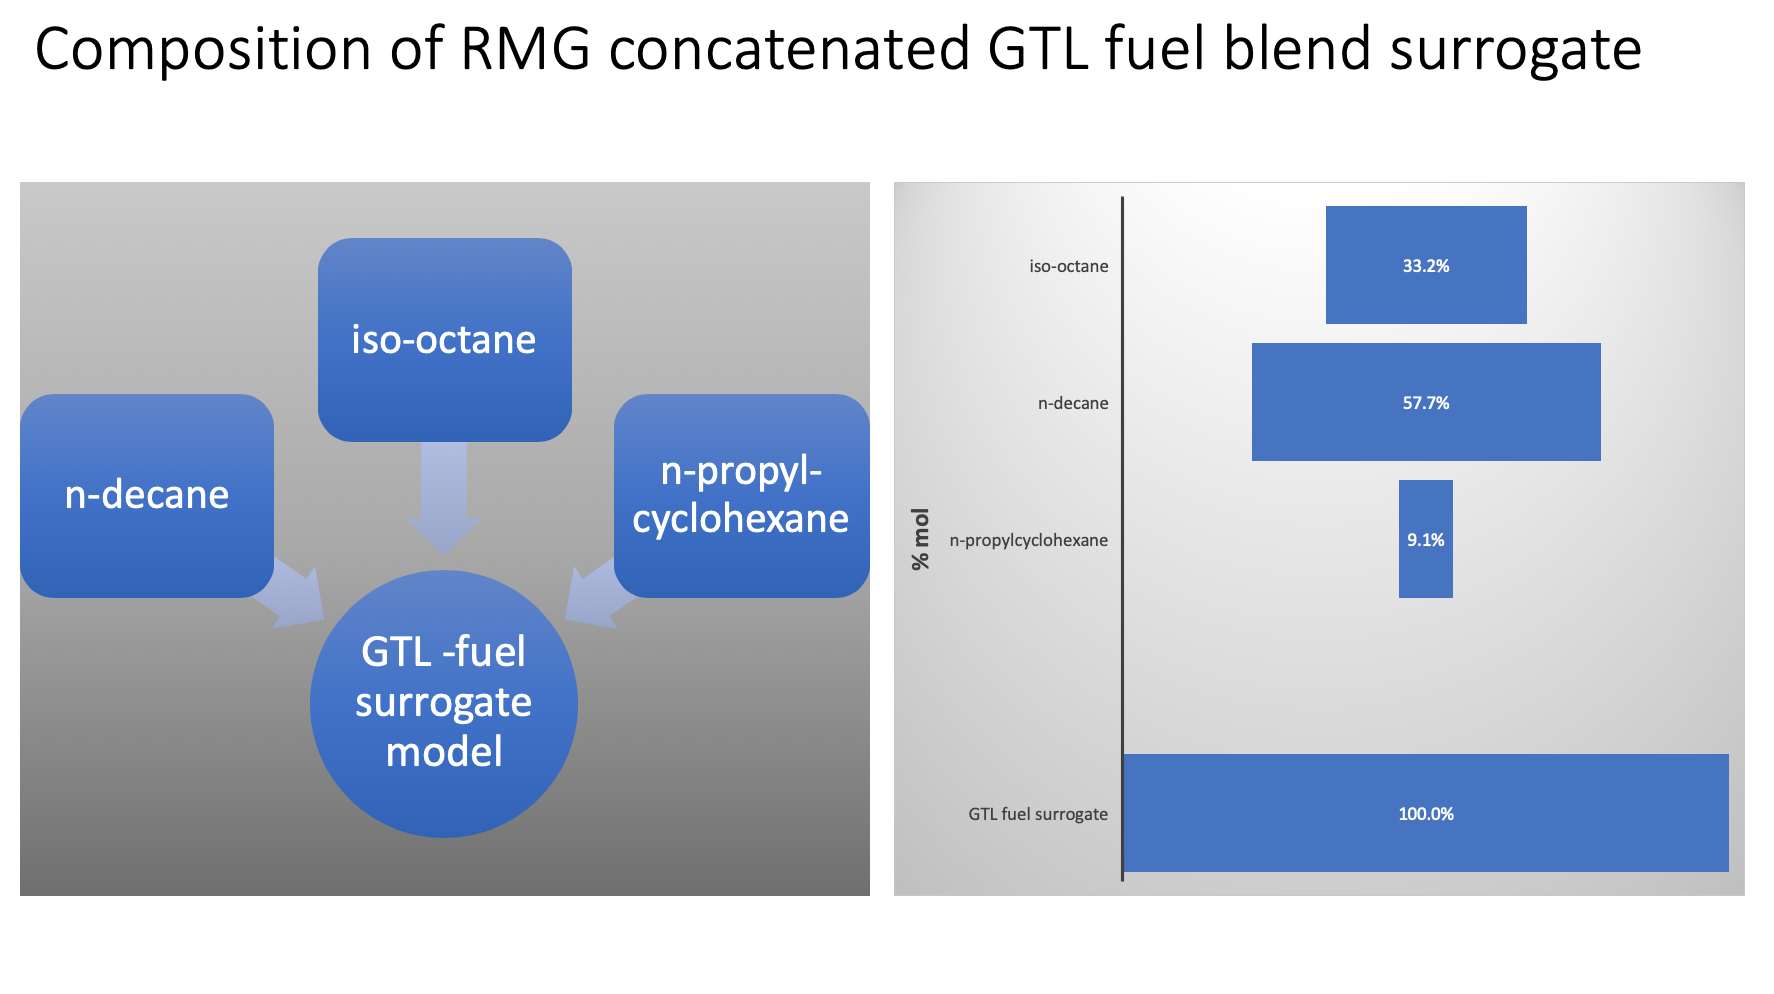
\includegraphics[scale=0.5,keepaspectratio]{images/GTL-Constituents.png}
    \caption{Composition of RMG concatenated GTL fuel surrogate model from the detailed mechanisms of n-decane, iso-octane and propyl-cyclohexane}
    \label{fig:gtl-surrogate}
\end{figure}


The second method involves a GTL fuel surrogate model that is constructed with all input species added from the onset such that cross-reactions are allowed shown in fig.\ref{fig:gtl_cross_rxn}. 

\begin{figure}
\hspace*{-2cm}
    \centering
    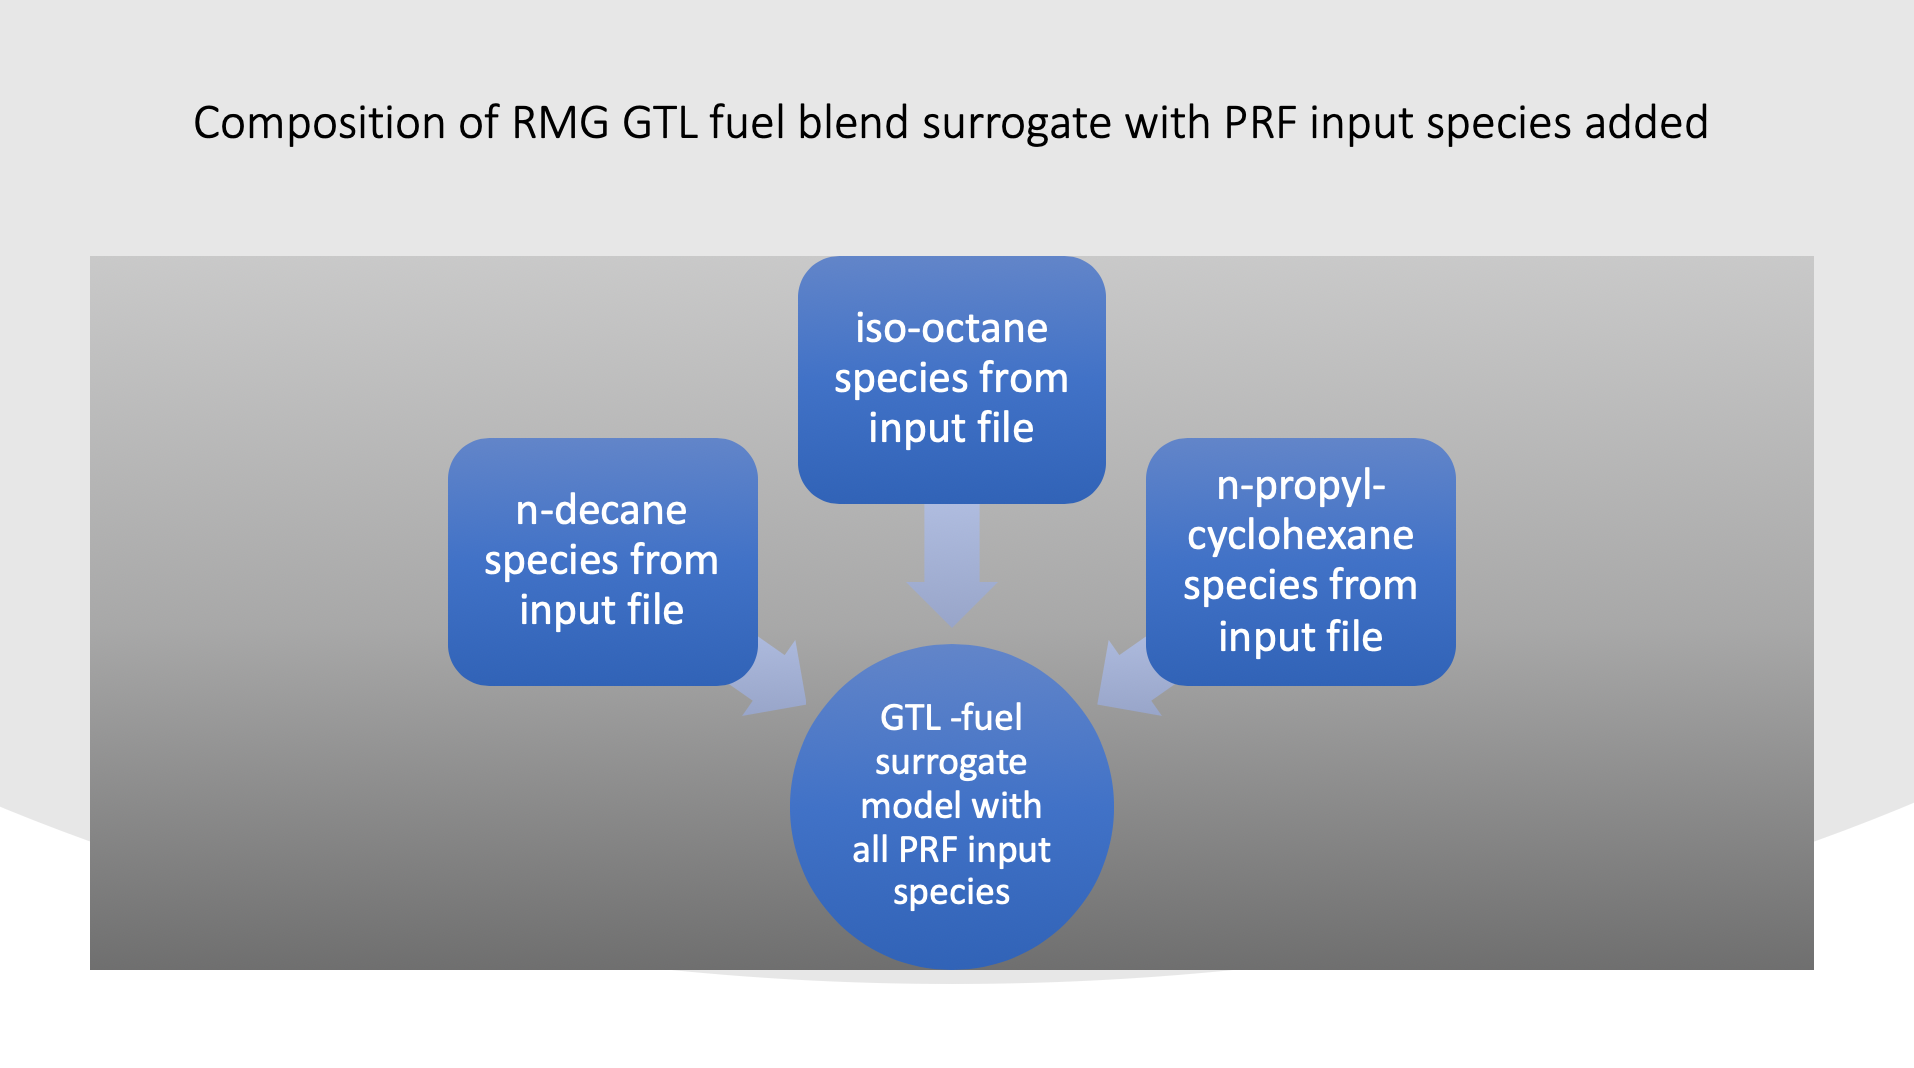
\includegraphics[scale=0.5, keepaspectratio]{images/GTL-cross-rxn.png}
    \caption{Illustration of GTL fuel surrogate model from the input species of PRFs}
    \label{fig:gtl_cross_rxn}
\end{figure}
\chapter{N-decane model}
\section{Kinetic Model}


Liquid transportation fuels are continuously used in different applications and the necessity to understand the reactivity of those fuels has been explored extensively in Chapter 1. Now we turn to the actual oxidation of the first primary reference fuel (PRF) of this work, which is n-decane. N-decane is a member of the straight chain hydrocarbons with the functional group alkane (aliphatics). It is named using the IUPAC nomenclature alongside the Greek root word ``dec" meaning ten. Thus, decane is a 10-membered straight chain hydrocarbon. The structure of decane looked at in this work is the normal-straight chain decane, implying no branching of the carbon chain as seen in the skeletal structure of fig.\ref{fig:decane}. Decane has the molecular formula of \ce{C_{10}H_{22}} since it is a member of the alkane family with a general structural formula of \ce{C_nH_{2n+2}}. 

\begin{figure}
    \centering
    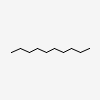
\includegraphics{images/Decane_100.png}
    \caption{Decane Structure}
    \label{fig:decane}
\end{figure}

\vspace{2.5cm}


n-Decane has long been identified as a constituent compound in the representation of transportation fuels \cite{Dooley2010AProperties}. Since it is representative of the important compounds in transportation fuels, enormous work has been done on the auto-ignition characteristics of the fuel. Experimental investigation of n-decane includes ignition delay time measurements in shock tubes and rapid compression machines (RCM)  \cite{Pfahl1996Self-ignitionConditions}\cite{Malewicki2013ExperimentalN-dodecane}\cite{Zhukov2008AutoignitionPressure}\cite{Horning2002StudyMixtures}\cite{Shen2009APressures}\cite{Dean2007AutoignitionPressures}\cite{Olchanski2006DecaneTube}\cite{Kumar2009AutoignitionConditions}\cite{Haylett2012IgnitionTube}, laminar flame speeds \cite{Zhao2004BURNING-DECANE}\cite{KUMAR2007209}\cite{Ji2010PropagationFlames}\cite{Moghaddas2012LaminarPressures}\cite{Hui2013LaminarPressures}\cite{Singh2011ExperimentalFlames}, chemical structure from pyrolysis and oxidation in pressure flow reactors \cite{Zeppieri2000ModelingPyrolysis}\cite{Jahangirian2012APressures}\cite{Zeng2014ExperimentalN-decane}\cite{Gong2014ExperimentalN-decane}, oxidation and pyrolysis in shock tubes \cite{Malewicki2013ExperimentalN-dodecane}\cite{Tekawade2016Time-resolvedN-dodecane} and oxidation in a jet stirred reactors \cite{Herbinet2013LowN-decane}\cite{Dagaut2008OxidationStudy}\cite{Battin-Leclerc2008DetailedSurrogates}\cite{Biet2008ExperimentalAlkanes}. These experimental measurements provide a basis with which to compare chemical kinetic models of n-decane as means of validating the mechanisms. Similarly, several kinetic models of n-decane have been published over the years using the chemical kinetic mechanism generation code EXGAS \cite{Warth2000ComputerOxidation} used by Battin-Leclerc and others \cite{Battin-Leclerc2000ModelingK}\cite{Biet2008ExperimentalAlkanes}, models have also been published on n-decane using the CHEMKIN suite code from Malewicki et al \cite{Malewicki2013ExperimentalN-dodecane}, n-decane model has also been deduced based on surrogate modeling of jet aviation fuels using a three-component fuel surrogate model of n-decane, iso-octane toluene as described by Dooley et al \cite{Dooley2010MethylModel}. Westbrook et al \cite{Westbrook2009AN-hexadecane} published a combined model of n-octane to n-hexadecane, Wang et al then constructed a very detailed model that integrates various fuels including n-alkane, cycloalkanes and alkyl-cycloalkanes in the JetSurF v2.0 model \cite{Wang2010A2.0},Sarathy et al followed up with a more compact model of \ce{C_7} to \ce{C_{20}} \cite{Sarathy2011ComprehensiveC20}.Although, skeletal models of n-decane have been built in the past by Zepperi et al \cite{Zeppieri2000ModelingPyrolysis}, more recently, Chang et al \cite{CHANG20131315} built a skeletal n-decane model for faster and efficient analysis. All these n-decane models built have been validated against various experimental conditions and there is still ongoing work to determination of new pathways, reaction intermediates, better estimation of thermo-chemical parameters and rate constants for these kinetic models of n-decane. \par
\par

The n-decane model conditions as constructed in RMG has been outlined in Chapter 2 table \ref{tab:PRF_table1} as well as the reactor conditions used in table \ref{tab:PRF_table2} and table \ref{tab:PRF_table3}. This section is going to focus exclusively on the reaction pathways of n-decane from high-temperature reaction to low-temperature as well as the flux diagram of fig. \ref{fig:f2} of the RMG model validated against published experiments with comparison to other published n-decane kinetic models. The n-decane model constructed in RMG was done on the basis of seed mechanisms of 
Burke et al\cite{Burke2012ComprehensiveCombustion}, Hashemi et al\cite{Hashemi2016High-pressureMethane} and Li et al\cite{Li2017TheoreticalC2H4} in the exact order as shown. The major reaction pathways shown in fig.\ref{fig:n-alkane-pathway} were discovered using the schematic and work of Merchant et al.\cite{Merchant2015UnderstandingPropane}, which used propane as a basis for the discovery of reaction pathways. As a result of this discovery, Merchant et al. concluded that the same scheme could be applied to n-alkanes up to \ce{C12} with an additional product of cyclic ethers from the \ce{QOOH} radical when they undergo cyclic ether formation reactions - where radicals move from one hydrogen to the other and a ring is formed as well as the loss of the \ce{OH} radical.



\newpage

\section{Reaction Pathways of N-decane Kinetic Model}
N-decane follows the class of reactions for its oxidation starting with a hydrogen abstraction reaction, and further down through a series of steps. H-abstraction reactions occur at both high and low temperatures. These class of reaction was proposed by Curran et al.\cite{Curran1998AOxidation} in the oxidation mechanism of n-heptane. At high temperatures, H-abstraction reactions occur via a $\beta$-scission - simply meaning that when the H-atom is removed, the radical is formed on the adjacent carbon atom to ensure thermodynamic stability. Nonetheless, since at high temperatures, there is sufficient energy and collisions occur more rapidly, the radical though stable isomerizes and forms other radicals within the decyl radical atom with molecular formula \ce{C10H21}. These radicals eventually decompose further along the \ce{C-C} bonds and letting go of yet another hydrogen to form a double bond - olefins with another radical species, thus having a combination of
  \reaction{C-C-C^. \rightleftharpoons C=C + C}
This reaction family in RMG is represented as the R\textunderscore Addition\textunderscore MultipleBond.  Conversely, at low temperatures, the five decyl radicals first decompose again along the \ce{C-C} bond to form smaller alkyl radicals via the R\textunderscore Recombination reaction and these smaller alkyl radicals undergo reaction with\ce{O2} to form alkyl-peroxide radicals or \ce{ROO^.}.The various stages of the reactions are dependent on temperature, thus at higher temperatures the chain branching is not as complex, however at lower temperature many reaction pathways are possible. Since RMG has its own unique class of reaction families that assist in determining which reaction classes guide the fuel molecule to the products desired, we adopt Merchant et al.'s \cite{Merchant2015UnderstandingPropane} guide to following the oxidation of n-alkane fuels using the schematic of fig.\ref{fig:n-alkane-pathway} gives a pictorial illustration to find out the major reaction pathways of n-decane, especially at low temperatures. In addition, since the onset of ignition in the Negative Temperature Coefficient (NTC) region is of interest, we use the illustration of Merchant et al.\cite{Merchant2015UnderstandingPropane} and Curran et al.\cite{Curran1998AOxidation} to discover the pathways of low temperature reaction classes of n-decane. The summary of the reaction classes as proposed by Curran et al.\cite{Curran1998AOxidation} and the corresponding RMG reaction families that enable the discovery of those pathways.

% \chemfig{*6(----(---)-)}



The major reaction classes for all the elementary reactions include the following:
\begin{enumerate}
    \item Unimolecular fuel decomposition
    \item H-atom abstraction from the fuel
    \item Alkyl radical decomposition
    \item Alkyl radical + \ce{O2} to produce olefin + \ce{HO2} radical directly
    \item Alkyl radical isomerization
    \item Abstraction reactions from olefin by OH, H, O and \ce{CH3}
    \item Addition of radical species to olefin 
    \item Alkenyl radical decomposition
    \item Olefin decomposition 
    \item Addition of alkyl radicals to \ce{O2} 
    \item Alkyl peroxy radical isomerization \ce{RO_2 \rightleftharpoons RO_2H}
    \item R\ce{O2^{.} + HO_2^.=RO_2H + O_2}
    \item R\ce{O_2^{.} + H2O2=RO2H + HO_2^.}
    \item R\ce{O2^{.} + CH3O2^{.}=RO^{.} + CH3O^{.} +O2}
    \item \ce{RO2^{.} + $R^\prime$O2^{.} = RO^{.} + $R^\prime$O^{.} + O2}
    \item \ce{RO2H=RO^{.} + O^{.}H}
    \item \ce{RO^.} decomposition
    \item \ce{Q^{.}OOH=QO+O^{.}H} cyclic ether formation via cyclization of diradical
    \item \ce{Q^{.}OOH}=olefin+\ce{HO2^{.}} (radical site $\beta$ to OOH group)
    \item \ce{Q^{.}OOH}=olefin + carbonyl + \ce{O^{.}H} (radical site $\gamma$ to OOH group)
    \item Addition of O2 to \ce{Q^{.}OOH}
    \item Isomerization of \ce{O2^{.}QOOH} and formation of ketohdroperoxide and \ce{O^{.}H}
    \item Decomposition of ketohydroperoxide to form oxygenated radical species and \ce{O^{.}H}
    \item Cyclic ether reactions with \ce{O^.H} and \ce{HO2^.}
\end{enumerate}
 
\begin{figure}
\hspace*{-3cm}
    \centering
    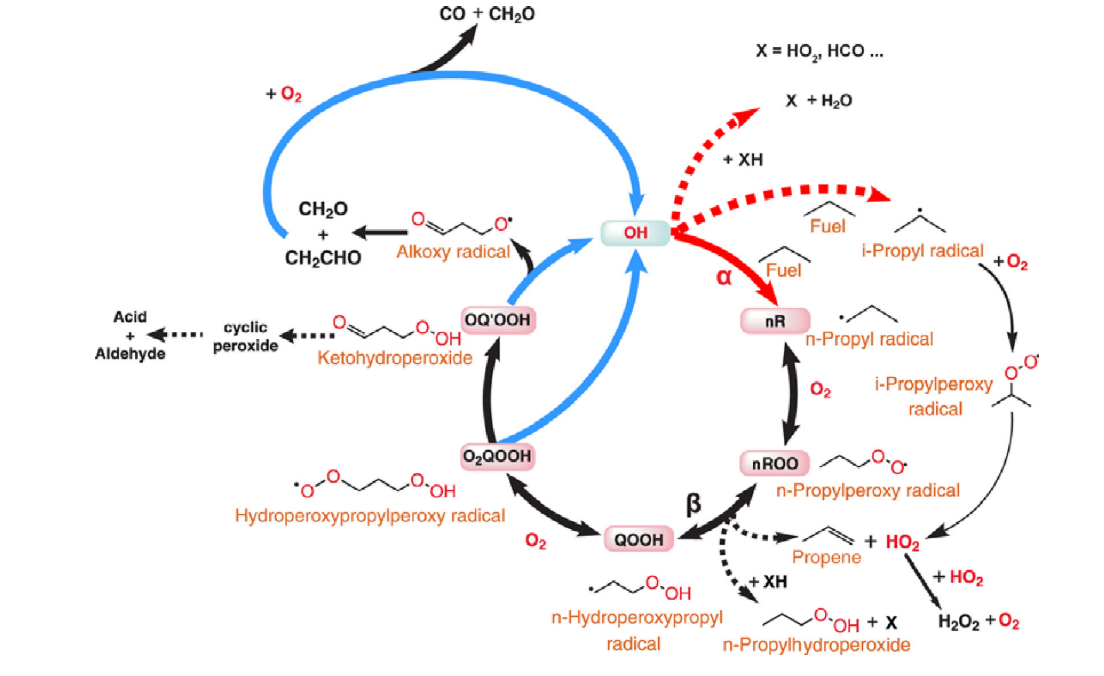
\includegraphics[scale=0.4, keepaspectratio]{images/rxn_class.png}
    \caption{Schematic of Merchant et al.\cite{Merchant2015UnderstandingPropane} major reaction pathways of propane during the first-stage of ignition. Reactions in blue lead to the formation of OH radicals. The reactions in dotted lines show competing pathways that divert radicals and lead to delay in the first-stage ignition}
    \label{fig:n-alkane-pathway}
\end{figure}

The convention of naming in this work is the R refers the the complete n-decane mechanism while $R^\prime$ refers to the alkyl radical as seen in \ce{C^.}, Q refers to the isomerized form of \ce{ROO^.} via an intra H-migration reaction with molecular formula \ce{C_nH_{2n}}. For the reaction classes, the rates used are those from the reaction libraries as outlined in the summary of table \ref{tab:PRF_table1} and the seed mechanisms also outlined in table \ref{tab:PRF_table1}. For the reaction \reaction{OH + H2O2 \longrightarrow HO2 + H2O}, which is normally described in a two-stage reaction step, for this work, the reaction is described in  a one-step reaction where the previous two-step reaction was taken from Burke et al. kinetic library \cite{Burke2012ComprehensiveCombustion} and the rate is from the work of Hong et al. \cite{Hong2010AOH}, indicates the rate dependency on only temperature and no significant pressure dependence between 1-2 atm. Hong et al. described the rate as the sum of two Arrhenius expressions over a temperature range of 280 to 1640 K.
The pre-exponential factor (frequency factor) of the Arrhenius expression of the one-step reaction rate of 
\reaction{OH + H2O2 \longrightarrow HO2 + H2O} was taken from the work of Honnet et al.\cite{Honnet2009AKerosene} which was equally taken from the work of Bikas et al.\cite{Bikas2001KineticAutoignition} and the work of Baulch et al. \cite{Baulch2005EvaluatedII} giving a preferred value of the rate as 
\begin{equation}
    k=2.72\times 10^{-6}exp(-\frac{14800}{T}) + 3.2\times 10^{-12}exp(-\frac{215}{T}) \hspace{0.5cm}  \text{cm}^3 \text{mol}^{-1} \text{s}^{-1}
\end{equation}


The summary of the rate parameters that were modified for this work is given in table 
\begin{table}[ht]
\arrayrulecolor[HTML]{DB5800}
\caption{Summary of RMG n-decane model reaction rate modifications with units of cm$^{3}$mol$^{-1}$s$^{-1}$, kcalmol$^{-1}$ }
\centering
\begin{adjustbox}{width=1\textwidth}
\begin{tabular}{ p{5cm} c c c c  c }
\rowcolor{lightgray}\multicolumn{5}{|c|}{RMG n-decane model Arrhenius expression reaction rates modification} \\
Reaction & Frequency factor (A) & Temperature exponent ($\alpha$) & Activation Energy ($E_A$) & Reference \\
\ce{OH + H2O2 \longrightarrow HO2 + H2O} & 7.8$\times$10$^{12}$ & 0.000 & 7.27 & \cite{Hong2010AOH}\cite{Burke2012ComprehensiveCombustion}\cite{Baulch2005EvaluatedII} \\
\ce{OH + HO2 \longrightarrow O2 + H2O} & 2.89$\times$10$^{13}$ & 0.000 & 0.497 & \cite{Keyser1988KineticsK}\cite{Baulch2005EvaluatedII}\cite{Burke2012ComprehensiveCombustion} \\
\ce{HO2 + HO2 \longrightarrow O2 + H2O2} & 4.2$\times$10$^{14}$ & 0.000 & -11.982 & \cite{Hippler1990ShockK}\cite{Burke2012ComprehensiveCombustion}\cite{Baulch2005EvaluatedII}\\
\ce{HO2 + HO2 \longrightarrow O2 + H2O2} & 1.3$\times$10$^{11}$ & 0.000 & 1.629 & \cite{Hippler1990ShockK}\cite{Burke2012ComprehensiveCombustion}\cite{Baulch2005EvaluatedII}\\
\ce{OH + CH2O \longrightarrow H2O + HCO} & \begin{tabular}{ c }
     3.559$\times$10$^{9}$  \\
     1.854$\times$10$^{9}$ \\
     1.070$\times$10$^{9}$ \\
\end{tabular} & \begin{tabular}{ c }
     1.167  \\
     1.256 \\
     1.330 \\
\end{tabular} & \begin{tabular}{ c }
     0.206  \\
     0.302 \\
     0.392 \\
\end{tabular} & \cite{Hashemi2016High-pressureMethane} \\
\end{tabular}
    \end{adjustbox}
    
    \label{tab:n-decane_model_rates}
\end{table}


\subsection{High Temperature Mechanism}

The high temperature mechanism can be accurately described with reaction classes 1-9.
\subsubsection{Unimolecular Fuel Decomposition and H-Abstraction Reactions} 
These reactions produce five alkyl radicals with the radical changing from one carbon atom to the next as well as an extra \ce{H} atom. Since the H atom abstraction reactions require high activation energies, they tend to favor the reverse direction as they serve as sink of H atoms. This initiation reactions are often observed in high temperature and pressure experiments such as that of shock tubes. In RMG, this reaction family is described by the H-Abstraction family with the general form 

\reaction{R^{1}-H^{2} + R^{3}\cdot \rightleftharpoons R^{1}\cdot {+} H^{2}-R^{3}\hspace{1cm} \text{H\textunderscore Abstraction reaction family}}


\subsubsection{Alkyl Radical Decomposition Reactions}
Alkyl radical decomposition reactions involve the breaking of the previously generated alkyl radical along the C-C bonds and is only relevant at high temperatures $>$ 850 K \cite{Curran1998AOxidation}. There is competition usually between this reation pathway and the addition of \ce{O2} to the alkyl radicals because of the low energy barrier for the addition of \ce{O2}, the pathway to give ROO can sometimes be favored. However, for larger alkanes > C8 the breaknig of the alkyl radical usually occurs via the $\beta$-scission to aid for the addition of the \ce{O2}. This reaction often leads to the formation of olefins (alkenes) or C=C double bonds as well as another radical. This reaction family is described in the RMG reaction family as radical recombination as the breaking down of the C-C bond usually favors the reverse direction with a general form as this 

\reaction{{R^{1}\cdot {+} R^{2}\cdot \rightleftharpoons R^{1}-R^{2}} \hspace{1cm} \text{R\textunderscore Recombination reaction family}}

\subsubsection{Alkyl Radical + \ce{O2} = Olefin + \ce{HO2^{.}} and Alkyl Radical Isomerization Reactions}

The reaction of alkyl radicals with \ce{O2} can undergo through various reaction paths. The reaction channel usually involves the addition of \ce{O2} in the form of \ce{O^{.}-O^.} where Oxygen is represented as a biradical singlet since this is the most stable form in its electronic structure. This reaction adds to the alkyl radical via the radical recombination channel and forms a alkylperoxy radical which then undergoes an isomerization to form a hydroperoxy-alkyl radical with the loss of a hydrogen atom. This new form is often labeled as \ce{QOOH} where the Q usually denotes the presence of a double bond. The reaction family of the first step from alkylperoxy radical to hydroperoxy-alkyl radical is the intra\textunderscore H\textunderscore migration and then finally to form the double bonded olefin is the R\textunderscore Addition\textunderscore MultipleBond.

\reaction{{H^{3}-R^{2}\thicksim R^{1}\cdot \rightleftharpoons R^{2}\cdot\thicksim R^{1}-H^{3}} \hspace{1cm} \text{intra\textunderscore H\textunderscore migration reaction family}} 
\reaction{R^{2}=R^{1} + R^{3}. \rightleftharpoons R^{2}.-R^{1}-R^{3}\hspace{1cm} \text{R\textunderscore Addition\textunderscore MultipleBond reaction family}}


Reaction classes 4-9 deal entirely with reactions of olefins. Since at high temperatures, the steric considerations are complex in the reaction channels, more emphasis is left on this reactions as the rate expressions are very complex in describing the pathways.

\subsection{Low Temperature Mechanism}
The low temperature mechanism can be described as reactions at temperatures $<$ 900 K with reaction classes 10-24.

\subsubsection{Addition of alkyl radicals to \ce{O2} and Alkyl peroxy radical isomerization \ce{RO2 \rightleftharpoons RO2H}}

The $\beta$-scission high activation energies makes reactions much slower, thus reactions with lower activation energies take precedence. The first is the addition of oxygen \ce{O2} to the alkyl radical and then isomerization reactions on the ROO radicals occur throughout the radical moving the radical sites with a \ce{H}-atom shift (internal H-abstraction) on the radical. 
\reaction{H^{3}-R^{2}\thicksim R^{1}\cdot \rightleftharpoons R^{2}\cdot\thicksim R^{1}-H^{3} \hspace{1cm} \text{intra\textunderscore H\textunderscore migration reaction family}} However, these internal H-abstraction reactions (H-migrations) are rather slow at lower temperatures thus making the addition of ROO decomposition to yield two reactive reactive hydroxyl radical and a carbonyl group. Evidently, Pollard \cite{Pollard1977Hydrocarbons} carried out extensive low temperature kinetic analysis of hydrocarbon oxidations and mapped out the most important features of low temperature submechanism. Many recent models have integrated these features in their models for simplifications essential for the oxidation of low temperature hydrocarbons. 



\subsubsection{Radical decomposition of \ce{RO2H \rightleftharpoons RO^{.} + O^{.}H} and \ce{Q^{.}OOH \rightleftharpoons QO + O^{.}H} }
The first step of the decomposition of \ce{RO2H} alkyl-hydroperoxides is one of the very important steps in the process of hydrocarbons and often controls the onset of a Negative temperature coefficent (NTC) regime in the auto-ignition of hydrocarbons. Thus, the production of the \ce{O^{.}H} radicals is necessary for the first-stage ignition process \cite{Merchant2015UnderstandingPropane} as well as the optimization process for cetane sensitizer improvements \cite{Curran1998AOxidation}. In order to form the alkenyl-hydroperoxy radicals \ce{Q^{.}OOH} from the alkyl-peroxides \ce{RO2}, unimolecular isomerizations occur again via the intra\textunderscore H\textunderscore migration reactions. 

When the alkoxy radicals are produced \ce{RO^.} from the decomposition of the alkyl-hydroperoxides \ce{RO2H}, they often tend to be unstable and decompose more readily to the stable form of oxygenated alkoxy radicals for large carbon chains often $>$ C8 with the presence of carbonyl groups such as aldehydes and ketones and other smaller alkoxy radical species via the intra\textunderscore H\textunderscore migration reaction family. The smaller alkyl radicals decompose even further eventually following a $\beta$-scission to form olefins (alkenes) via the R\textunderscore Addition\textunderscore MultipleBond reaction family, which is stable in this form by the presence of its pi bonds. For the aldehydes, due to the presence of a double bonded oxygen, they are reactive and additions to the double bond are possible forming yet another alkyl radical and another oxygen radical which can attack double bonds. 


As the radical decomposition continues, the alkenyl-hyrdoperoxy radicals involves the breaking of the \ce{O-O} bond with the chain branching to form cyclic ethers with an extra \ce{O} atom in the chain.As the chain branching begins, cyclic ethers are formed with the loss of the internal \ce{H} from QOOH as a competing reaction pathway. The cyclic ether formation has a unique reaction family in the RMG database that forms from the \ce{QOOH} radical seen as \reaction{R^{1}^.\thicksim O^{2}-O^{3}-R  \rightleftharpoons R^{1}\thicksim O^{2} + O^{3}R^. \hspace{1cm} \text{Cyclic\textunderscore Ether\textunderscore Formation }} The presence of these cyclic ethers is shown in the schematic of Merchant et al.\cite{Merchant2015UnderstandingPropane} fig.\ref{fig:cyclic-ethers}. 

\begin{figure}[!ht]
\hspace*{-3cm}
    \centering
    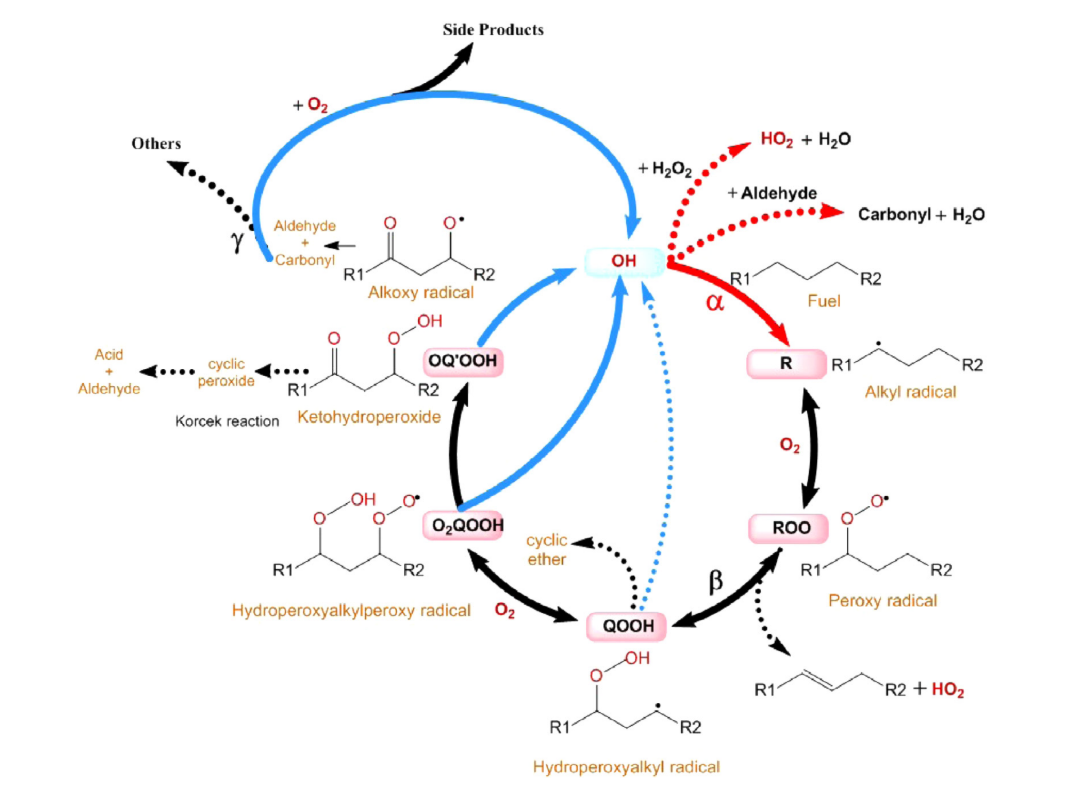
\includegraphics[scale=0.45, keepaspectratio]{images/nalkane-schematic+ROR.png}
    \caption{Schematic of low temperature oxidation of n-alkanes with the presence of cyclic ethers as shown by Curran et al.\cite{Curran1998AOxidation} and schematic from Merchant et al.\cite{Merchant2015UnderstandingPropane}}
    \label{fig:cyclic-ethers}
\end{figure}

\cleardoublepage

\subsubsection{Decomposition of \ce{Q^{.}OOH \rightleftharpoons Olefin + HO2^.} and \ce{Q^{.}OOH \rightleftharpoons Olefin + Carbonyl + O^{.}H}}

Alkenyl-hydroperoxide radicals \ce{Q^{.}OOH} have a $\beta$ radical site that can decompose to an olefin and hydroperoxy radical \ce{HO2^{.}} via an addition reaction along the \ce{Q-OOH} site. The \ce{HO2^.} radicals often play an important role in the auto-ignition process of hydrocarbons and contributes to the NTC behavior of n-decane. Similarly, rather than decomposition along the \ce{Q-OOH} site, $\beta$-scission can occur and the presence of olefins alongside a smaller carbonyl group usually a ketone and a hydroxy radical \ce{O^.H} is formed. These three body reactions usually have very high weak dependence on temperature and its rate estimates are often observed to be very close to the high pressure limit and violate the collision limits of the Lennard-Jones parameter as described by Chen et al.\cite{Chen2017ViolationModels}. 


\subsubsection{Addition of \ce{O2} to \ce{Q^.OOH} and Isomerization of \ce{O2^.QOOH} to Ketohydroperoxide and \ce{O^.H} radicals}
Alkenyl-hydroperoxide \ce{Q^.OOH} radicals can react with \ce{O2} via radical recombination reactions to form peroxy alkenyl-hydroperoxide radicals \ce{O2^.QOOH}. \reaction{R^{1}\cdot {+} R^{2}\cdot \rightleftharpoons R^{1}-R^{2} \hspace{1cm} \text{R\textunderscore Recombination reaction family}}
 
 Further chain branching steps of the peroxy-alkenyl-hydroperoxide radicals can form \ce{HOOQ^.OOH} dihydroperoxy-alkenyl radicals via an inernal H migration reaction before the final isomerization reaction to eliminate the \ce{O^.H} radicals and form different ketohyperoxide species depending on the carbon chain. The QOOH radicals alongside chain branching form a combination of carbonyl groups of ketones and olefins as well as OH radicals. The \ce{O2QOOH} species then isomerize to form ketohydroperoxides and OH radicals along the double bonds.  
 
 The full pathways integrating both the high and low temperature chemistry is seen in fig.\ref{fig:f2} of n-decane.

\begin{figure}[!htp]
    \centering
\hspace*{-3cm}
    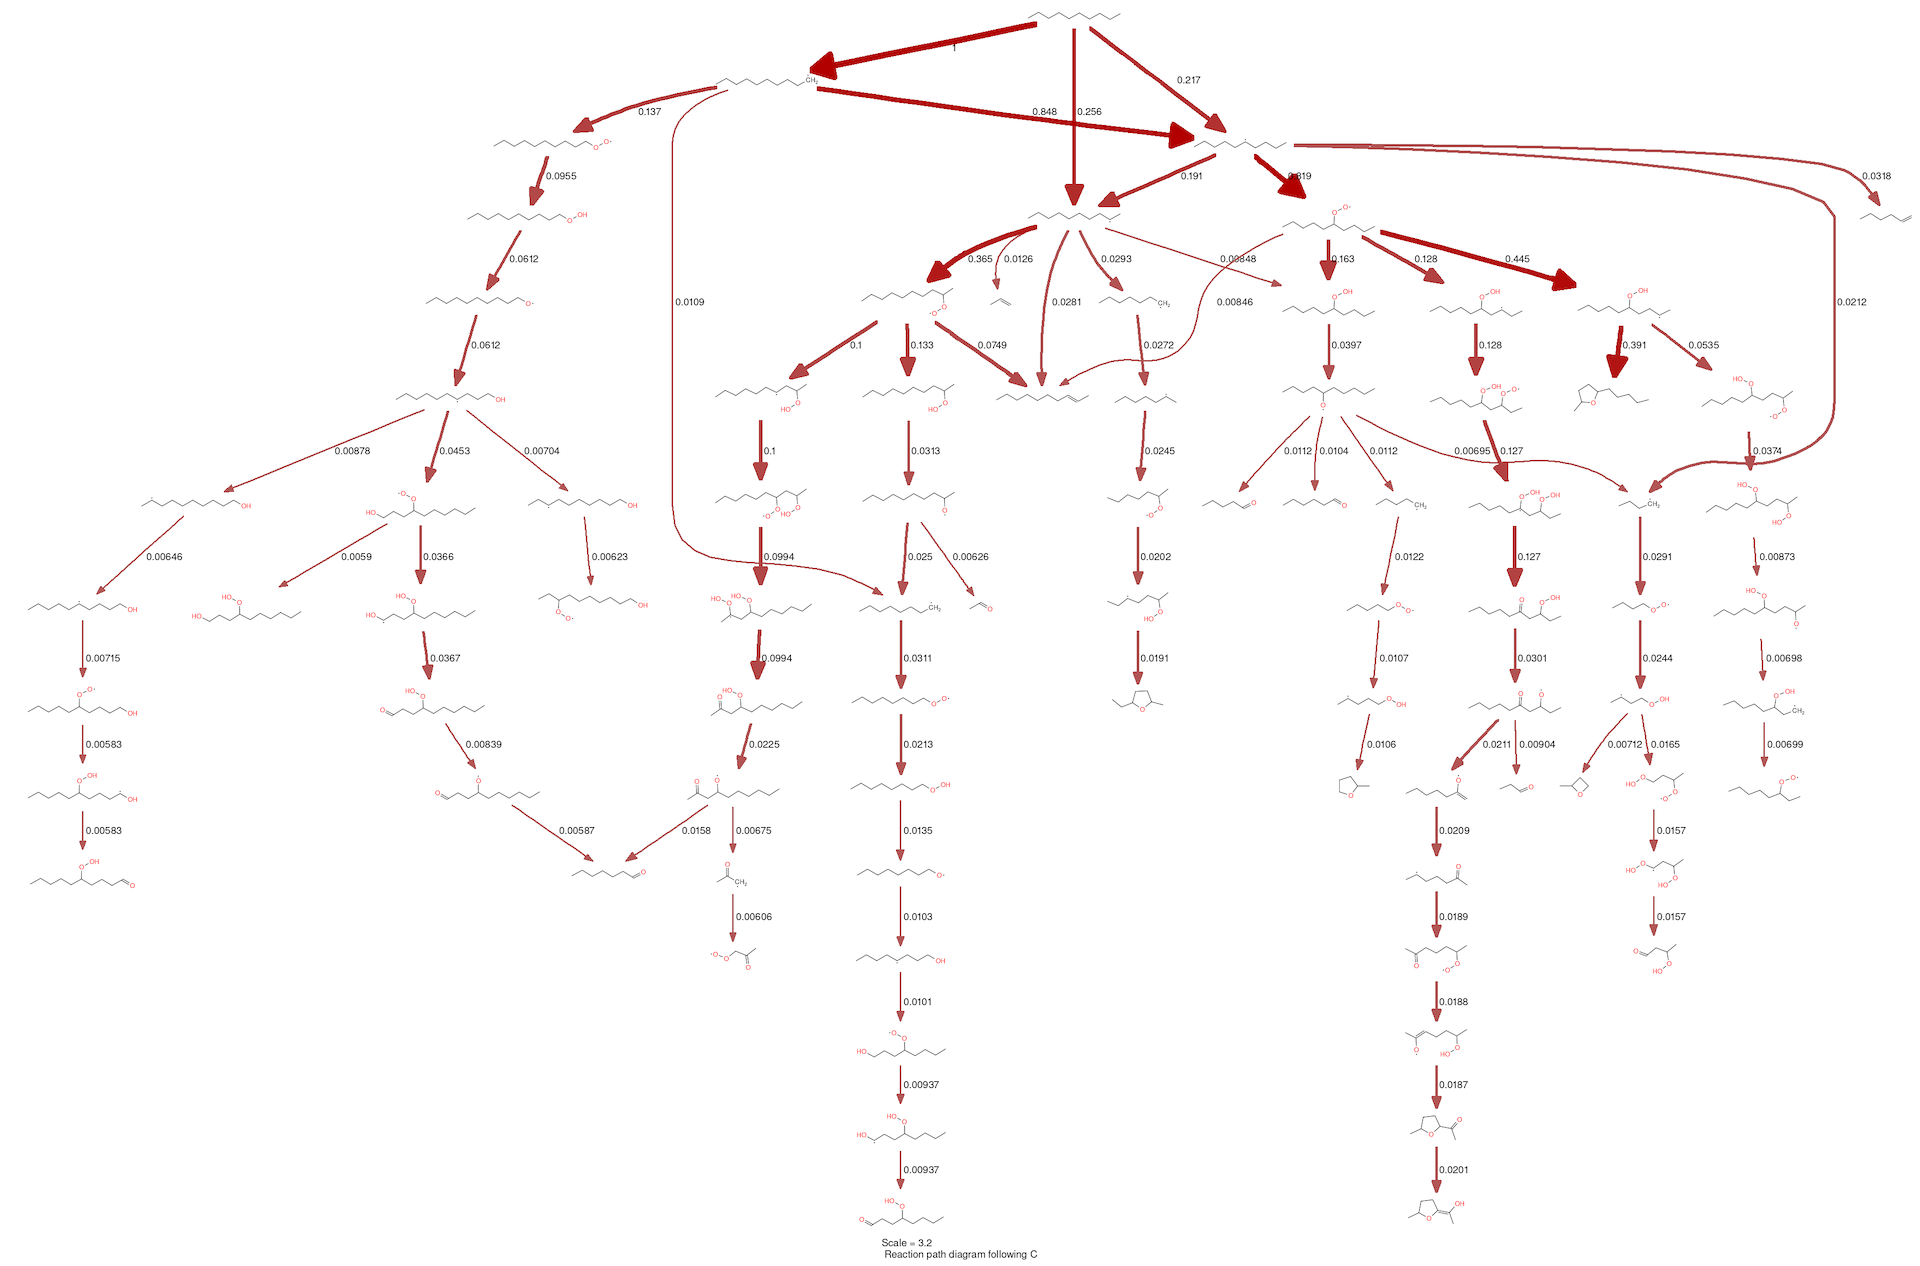
\includegraphics[scale=0.35,keepaspectratio]{images/nc10-rxn-path-800K.png}
    \caption{Flux diagram of n-decane @ 800K and 13 bar}
    \label{fig:f2}
\end{figure}


\newpage

\section{Model validation of n-decane under experimental conditions}
The detail of the model generation of n-decane using RMG has been described in sufficient detail with the inclusion of both the high temperature and low temperature reaction pathways as well as the model generation process algorithm highlighted in Chapter 2. Now we look into the validation of the n-decane model using the chemical kinetics code Cantera \cite{cantera}. First the model is validated against experiments of Shock Tubes for ignition delay time measurements and eventually flow reactors for laminar premixed flame speeds at a wide range of conditions.


\subsection{Model validation of n-decane in shock tubes for ignition delay time predictions}
Shock tubes essentially devices designed to experiment and study the flow of high-temperature and high-velocity effects of compressible gases within an actual engine-like environment. It is designed on the basis of knowledge of gas dynamics and analysing shock waves. It operates on the principle that at high temperatures, supersonic gases flow is in the tube a diaphragm causes a separation into regions of high-pressure and low-pressure. As the pressure rises, an unsteady rarefied wave passes into the driver gas with a velocity usually a few kilometers per second causing flow from the high-pressure region to the low-pressure region. As the shock wave progresses in the low-pressure region, it pushes the low-pressure gas ahead of it. Thus, creating two fronts, flow ahead of the shock wave and flow behind the shock wave. The flow ahead of the behind the shock wave (driver gas) is the gas of interest. The velocity of the driver gas is equal to  that of the driven gas\cite{Greene1964TheR.}. Usually, there in the high-pressure region, is an explosive gas which is the gas studied, and present is a laser beam to detect the luminescence of some excited species. The ignition delay time can be defined as the time it takes:
\begin{enumerate}
    \item For the shock wave to hit the wall and propagate with the excitation of a \ce{CH*} or \ce{OH*}radical
    \item For the shock wave to hit the wall and measurement of the highest peak of the temperature in the driven section
    \item For the shock wave to hit the wall and detection of the highest peak of the pressure in the driven section
\end{enumerate}
Since all three possibilities of measuring the ignition delay time data in shock tubes exist, it is often well defined based on one of the three main possibilities usually for the first-stage ignition \cite{Davidson2004InterpretingData}\cite{Fieweger1997Self-ignitionPressure}\cite{Pfahl1996Self-ignitionConditions}\cite{Haylett2012IgnitionTube}

In Cantera, this process is often defined based on the reactor type of interest. First, the gas solution object is created with the \textbf{gas.Solution} class, then a reactor type is selected with the appropriate initial conditions usually coming from the experimental data being validated against. Next, the state of the system is set with the reactor network previously defined and then a simulation in time for the next states is found using the ODE solver. The ODE solver starts at the current state  of the systems and progresses in time by one of the following methods:
\begin{enumerate}
    \item \textbf{step()}: This involves a reactor step from the current state of the system by solving the previous state of the system using the time step given. This is an explicit method where the ODE solver internally solves the numerical Differential Algebraic Equations (DAE) system. The new time is returned as well as the state of the system at the next state using the previously defined time step $\Delta$t within the solver absolute and relative tolerances. The time step cannot be larger than the maximum time step or else the ODE solver breaks.
    \item \textbf{advance($t_{new}$)}: This method solves the state of the system at a predefined step times $t_{new}$. This $t_{new}$ describes the absolute time of the system from the initial system by calling the ignition delay time function for the reactor in a loop, either a while loop or for loop at exactly the time specified - basically using the \textbf{step():} function several times in the process. In addition, the \textbf{advance():} function can be made to continue until a steady-state solution is attained by time stepping. Only when the feature-scaled residual of the state vector is below a given threshold value is the system at steady-state and the ODE solver stops.
\end{enumerate} 
For all shock tube models in this work, a zero-dimensional homogeneous closed ideal gas reactor with constant volume and internal energy class was used since at constant volume, there is no P-V work done against the control volume of the gas. Since the temperature is known, the energy equation is computed assuming adiabatic conditions in the reactor volume. The time integration of the species is computed in uniform time steps until the solution is found. During the time integration, the reactor model scheme usually an ODE SUNDIALS solver \cite{hindmarsh2005sundials} solves the differential equations of the species within the energy equation. The energy equation accounts for the energy interaction via the heat equation but is ignored since the reactor assumes adiabatic conditions and indicates only mechanical work interactions, mass transport due to species diffusion and conversion.  The equation being solved in the ideal gas reactor  of Cantera is equation \ref{eq.mass conservation} as given by Robert Kee et al's book on Chemically Reacting Flow \cite{Kee2003ChemicallyPractice}. The definition of the ignition delay time varies. Nonetheless, the model used in Cantera assumes an ignition delay time based on the excited \ce{CH} or \ce{OH} radical species and is often very close to the highest temperature spike Ji et al point out for the sensitivity analysis of ignition delay times \cite{Ji2019EvolutionAutoignition}. 

\begin{equation}
    U = m\sum_k{Y_k u_k(T)}
\end{equation}

\begin{equation}
    \frac{dU}{dt} = u\frac{dm}{dt}+mc_v\frac{dT}{dt}+m\sum_k{u_k \frac{dY_k}{dt}}
\end{equation}

\[\text{Substituting the corresponding derivations for temperature in the reactor as:} \]


\begin{equation}
    mc_v\frac{dT}{dt}=-p\frac{dV}{dt} - Q^. + \sum_{in}{m_{in}(h_{in}- \sum_k{u_k Y_{k, in}}) -\frac{pV}{m}\sum_{out}{m_{out}^.} - \sum_k{m_{k, gen}^. u_k}}
    \label{eq.mass conservation}
\end{equation}

The ignition delay times prediction are presented as modeled in Cantera against shock tube experiments of Pfahl et al\cite{Pfahl1996Self-ignitionConditions} in fig.\ref{fig:idt times}.

As seen in fig. \ref{fig:idt times}, there is good agreement between the model prediction of ignition delay times against the experiments of Pfahl et al. \cite{Pfahl1996Self-ignitionConditions}. Pfahl et al. studied the self-ignition of diesel relevant fuels between lean, stoichiometric and rich fuel mixture conditions in a high pressure shock tube and observed a transition from deflagration-like behavior to a  detonation-like behavior around 960 K with strong high pressure peaks, cool flame and onset of a NTC regime in a two-step ignition using both the maximum \ce{CH^*} excited band at 431nm and maximum temperature gradient $\frac{\partial T}{\partial t}$ in a zero dimensional reactor.

\begin{figure}[!hbp]
    \centering
    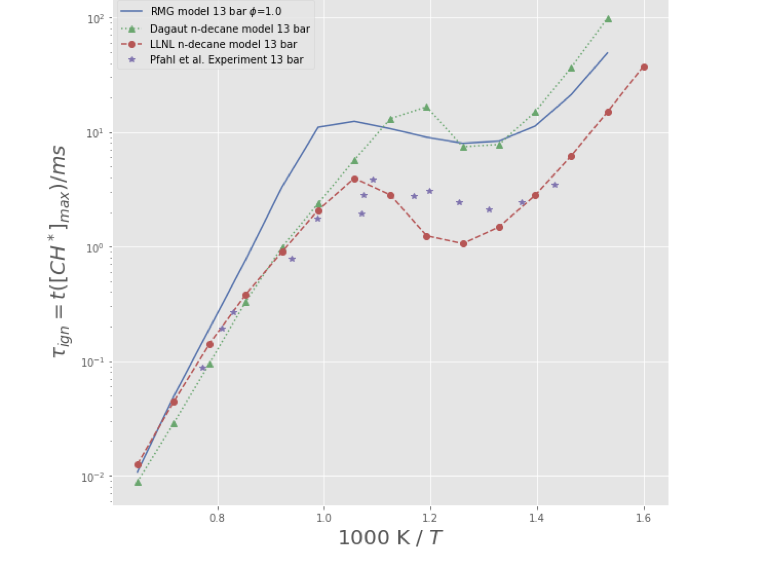
\includegraphics[scale=0.4, keepaspectratio]{images/idt_nc10_13bar.png}
    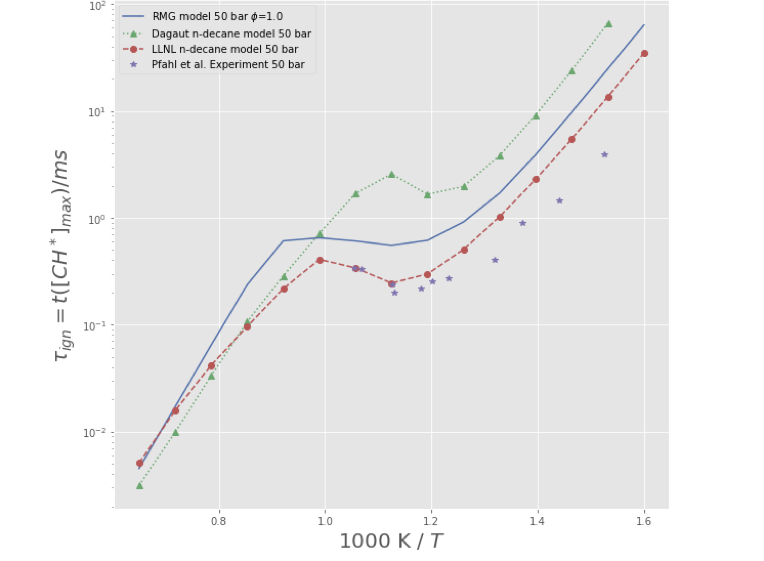
\includegraphics[scale=0.4, keepaspectratio]{images/idt_nc10_50bar.png}
    \caption{Ignition delay time prediction of n-decane/air at 13 bar and 50 bar for $\phi=1$ stoichiometric mixtures against models of LLNL from Sarathy et al.\cite{Sarathy2011ComprehensiveC20}, Dagaut et al. GTL fuel surrogate model \cite{Dagaut2014} and experiments of Pfahl et al. \cite{Pfahl1996Self-ignitionConditions}. Lines indicate model predictions and stars indicate experiments}
    \label{fig:idt times}
\end{figure}

\cleardoublepage
\subsubsection{Sensitivity Analysis of the Ignition delay times}
A detailed analysis was done to determine which control variables control the ignition delay of the n-decane model. Since the species usually measured for the onset of ignition is the \ce{OH^.} radical, the concentration of the \ce{OH^.} radical was used as the criteria for sensitivity by the use of a brute force method comparing the localised sensitivity at a given temperature for all the top reactions that influence the ignition delay time. This sensitivity analysis was done at high temperatures of 1300 K, intermediate temperatures of 900K and at low temperatures of 700K to observe which reactions contribute the most to either the production or consumption of the \ce{OH^.} radical species. The sensitivity analysis involves the perturbation of both the forward and reverse rates of the 20 most sensitive reactions to \ce{OH^.} radical concentration by a factor of two and then comparing the change in the ignition delay time to the preset rate constant of those same reaction sensitivity to the \ce{OH^.} radical species. The magnitude of the sensitivity coefficient indicates a strong dependence on \ce{OH^.} radical concentration, while the sign indicates rate of production if positive and rate of consumption if negative. The sensitivity plots are shown in fig.\ref{fig:nc10-sensitivity}.

The summary of the RMG n-decane model is given in table \ref{tab:n-decane_model_summary}. 
\begin{table}[ht]
\arrayrulecolor[HTML]{DB5800}
\caption{Summary of RMG n-decane model analysis and Ignition delay time prediction at extinction }
\centering
\begin{adjustbox}{width=1\textwidth}
\begin{tabular}{ p{6cm} c c c c }
\rowcolor{lightgray}\multicolumn{4}{|c|}{RMG n-decane model summary} \\
Number of Species before sensitivity analysis & 331 & &  \\ 
Number of species after sensitivity analysis  & 331 & &  \\
Number of Reactions before Sensitivity analysis & 7381 & & \\ 
Number of reactions after sensitivity analysis & 7380 & & \\ 
\hline
 Model ignition delay time at extinction &  Temperature & Pressure & Equivalence ratio \\
 \begin{tabular}{ c }
    $\tau$=59.7355 ms   \\
    $\tau$=47. 2724 ms \\ 
    $\tau$=87.1198 ms \\
 \end{tabular} & \begin{tabular}{ c } 
       682.92 K\\
      652.68 K \\
      625 K \\
 \end{tabular} & 13 bar & \begin{tabular}{ c }
      0.5 \\
      1.0 \\
      2.0 \\
 \end{tabular} \\
 \begin{tabular}{ c }
    $\tau$=43.0018 ms \\
    $\tau$=63.286 ms \\
    $\tau$=44.5987 ms \\
 \end{tabular} & \begin{tabular}{ c }
      652.68 K \\
      625 K \\
      625 K \\
 \end{tabular} & 50 bar & \begin{tabular}{ c }
      0.5 \\
      1.0 \\
      2.0 \\
 \end{tabular}\\
\end{tabular}
    \end{adjustbox}
    
    \label{tab:n-decane_model_summary}
\end{table}


\begin{figure}
    \centering
    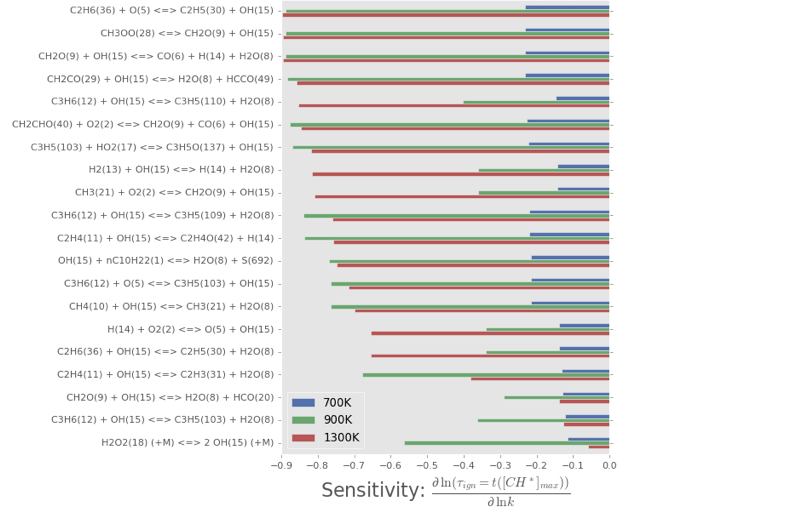
\includegraphics[scale=0.5, keepaspectratio]{images/sensitivity-nc10.png}
    \caption{Sensitivity coefficients of the ignition delay time of the n-decane model to \ce{OH^.} radical concentration at stoichiometric fuel/air mixture at 700 K, 900 K, 1300 K at $P=13$ bar. Where the ignition delay times $\tau_{ign}=t(\ce{CH^.}_{max})$}
    \label{fig:nc10-sensitivity}
\end{figure}


\begin{figure}
    \centering
    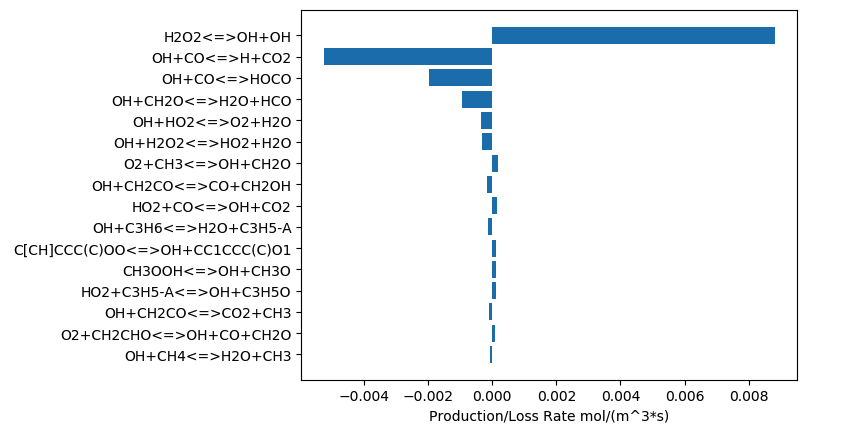
\includegraphics[scale=0.45, keepaspectratio]{images/ROP_nc10.png}
    \caption{Rates of Production/Consumption of the \ce{OH^.} radicals of the n-decane model}
    \label{fig:rop-nc10}
\end{figure}

\newpage

\subsection{Model validation of n-decane for Laminar Premixed Flame Speeds}
The RMG model of n-decane has been validated against experimental data of Pfhal et al.\cite{Pfahl1996Self-ignitionConditions} for ignition delay times and laminar flame speeds of Kumar et al.\cite{KUMAR2007209}, Hui et al.\cite{Hui2013LaminarPressures} and Ji et al.\cite{Ji2010PropagationFlames}. The model itself was also compared with model predictions of Lawrence Livermore National Laboratories (LLNL) n-decane model as provided by Sarathy et al\cite{Sarathy2011ComprehensiveC20} and the GTL surrogate model of Dagaut et al.\cite{Dagaut2014}. A summary of the n-decane model of the current study as constructed in RMG is provided in table \ref{tab:n-decane_validation_summary}. 



\begin{table}[!hbp]
\arrayrulecolor[HTML]{DB5800}
\caption{Summary of the experiments and operating conditions validated with RMG n-decane model. * For laminar flame speeds of Kumar et al.\cite{KUMAR2007209} at $T_u$=400K only pressure at 1 atm was compared to the experiments }
\centering
\begin{adjustbox}{width=1\textwidth}
\begin{tabular}{ p{5cm}  p{5cm} p{5cm} p{5cm} p{5cm} p{5cm} }
    \rowcolor{lightgray} \multicolumn{5}{|c|}{RMG n-decane model experimental validation summary} \\
    Operating Conditions & Temperature & Pressure & Equivalence ratio & Reference  \\
    Ignition delay Times & \begin{tabular}{ c }
         1239-1616 K \\
         990-1320 K \\
         680-1210 K  \\
         700-1810 K \\
         700-1290 K \\
    \end{tabular} & \begin{tabular}{ c }
         1.82-10 atm  \\
         10 atm, 35 atm \\
         13 bar, 50 atm, 80 atm \\
         5-80 atm \\
         13 bar \\
    \end{tabular} & \begin{tabular}{ c }
         0.7-3.0  \\
         0.25 \\
         0.5 \\
         1.0 \\
         2.0 \\
    \end{tabular} & \begin{tabular}{ c }
         \cite{Olchanski2006DecaneTube} \\
         \cite{Shen2009APressures} \\
         \cite{Pfahl1996Self-ignitionConditions},\cite{Zhukov2008AutoignitionPressure},\cite{Shen2009APressures} \\
         \cite{Pfahl1996Self-ignitionConditions},\cite{Dean2007AutoignitionPressures},\cite{Zhukov2008AutoignitionPressure}, \cite{Shen2009APressures},\cite{Haylett2012IgnitionTube} \\
         \cite{Pfahl1996Self-ignitionConditions} \\
    \end{tabular} \\
    Laminar flame speeds & \begin{tabular}{ c }
         $T_u$= 360 K \\
         $T_u$= 400 K \\
         $T_u$= 403 K \\
         $T_u$= 470 K \\
    \end{tabular} & \begin{tabular}{ c }
         1 atm \\
         1*, 2, 3 atm \\
         1 atm \\
         1 atm \\
    \end{tabular} & \begin{tabular}{ c }
         0.7-1.4 \\
         0.7-1.4 \\
         0.7-1.5 \\
         0.7-1.3 \\
    \end{tabular} & \begin{tabular}{ c }
         \cite{KUMAR2007209} \\
         \cite{KUMAR2007209},\cite{Hui2013LaminarPressures} \\
         \cite{Ji2010PropagationFlames} \\
         \cite{KUMAR2007209} \\
    \end{tabular} \\
\end{tabular}
    \end{adjustbox}
    
    \label{tab:n-decane_validation_summary}
\end{table}

The flame modeling in Cantera uses the same ODE solver of SUNDIALs \cite{hindmarsh2005sundials}, however the governing equations are different. For the laminar premixed flame speed simulations, the flow is restricted to a one-dimensional flame by the use of a similarity solution. While the flame model done in this work for RMG is that of a freely-propagating laminar premixed flame, the solution class differs by the state of the control volume of the flame. The Cantera class \textbf{cantera.FreeFlame} is used for this analysis and assumes an ideal gas flow of the flame, where the flame is actually stationary but the species diffuse into and out of the stationary flame. The other argument of the \textbf{cantera.FreeFlame} class is the grid and width of the flame. This uses the grid nodes to determine the accuracy of the flame solved while the width determines the interval over which the grid is defined. Numerical accuracy often correlates to having more grid points, however this quest for accuracy comes at a very high computational cost. The number of grid points used in evaluating this n-decane flame speed model is included in a table \ref{tab:n-decane_gridpoints}. Flames in Cantera are computed along the stagnation streamlines, indicating that the flow is gas dynamically incompressible and irrotational. The following governing equations are used for the flame model in Cantera.
\[\text{Continuity or Mass conservation}\]
\begin{equation}
    \frac{\partial \rho u}{\partial z} + 2\rho V = 0
\end{equation}

\[\text{Radial momentum from the Navier-Stokes Equation of flow fields with stress tensor}\]
\begin{equation}
    \rho u\frac{\partial V}{\partial z} + \rho V^2 = -\Lambda + \frac{\partial}{\partial z}(\mu \frac{\partial V}{\partial z})
\end{equation}

\[\text{Energy equation as a function of temperature}\]
\begin{equation}
    \rho c_p u\frac{\partial T}{\partial z}=\frac{\partial}{\partial z}(\lambda \frac{\partial T}{\partial z})-\sum_k{j_k c_{p,k}\frac{\partial T}{\partial z}} - \sum_k{h_k W_k\Dot{\omega_k}}
\end{equation}

\[\text{Species conservation}\]
\begin{equation}
    \rho u\frac{\partial Y_k}{\partial z}=-\frac{\partial j_k}{\partial z} + W_k\Dot{\omega_k}
\end{equation}

Where $\rho$ is the density of the reacting flow species, u is the $u$ is the axial velocity, $V=v/r$ is the scaled radial velocity and $v$ is the radial velocity, $\Lambda$ is the pressure eigenvalue (independent of z in the axial direction), $\mu$ is the dynamic viscosity, $c_p$ is the specific heat capacity at constant pressure, $T$ is the temperature, $\lambda$ is the thermal conductivity, $Y_k$ is the mass fraction of species $k$, $j_k$ is the diffusive mass flux of species $k$, $c_{p,k}$ is the specific heat capacity of species $k$ at constant pressure, $h_k$ is the species enthalpy, $W_k$ is the relative molecular weight of species $k$ and $\Dot{\omega_k}$ is the molar production of species $k$. \hfill \break 


The boundary conditions are often defined at the inlets and outlets of the control volume. For an inlet boundary condition, the following equation is solved based on the imposed conditions of the flame.
\[\text{Inlet boundary}\]
For the boundary points where $z_0$ is the starting point of the computational grid, the values are usually imposed for the initial parameters such as temperature $T_0$, species mass fraction $Y_{k,0}$ the scaled radial velocity $V_0$ since this is a freely propagating flame, initial mass flow rate $m_0$ is not given since species diffuse in and out of the flame. This numerical boundary condition is known as a Dirichlet boundary condition.

\begin{align}
    T(z_0)=T_0   \\
    V(z_0)=V_0
\end{align}

\begin{equation}
    \Dot{m_0}Y_{k,0}-j_k(z_0)-\rho(z_0)u(z_0)Y_k(z_0)=0
\end{equation}

Since the initial mass flow rate is not given for a freely propagating flame it is not included.\\ Nonetheless,if it is given as:

\begin{equation}
    \Dot{m_0}=\rho(z_0)u(z_0)
\end{equation}
 
\[\text{in addition, the pressure gradient can be solved as:}\]
\begin{equation}
    \Lambda(z_0)=0
\end{equation}

For a boundary at $z_0$ with an outflow, the temperature, species mass fraction and pressure gradients are used as boundary conditions from the Neumann boundary condition type. 
\[\text{Outlet boundary}\]
\begin{equation}
    \Lambda(z_0) = 0  
    \end{equation}
    \begin{equation}
       \frac{\partial T}{\partial z}|_{z_0}= 0  
    \end{equation}
    \begin{equation}
      \frac{\partial Y_k}{\partial z} |_{z_0} = 0   
    \end{equation}
    \begin{equation}
        V(z_0)=0
    \end{equation}
    


While the RMG n-decane model has a fairly large number of species and reactions, the various models with which it was compared with had more, especially since some of the models are from surrogates. The n-decane model of this work had originally 331 species and 7381 reactions. However, as the model validation began, using sensitivity analysis, some kinetic parameters were changed in order to produce a model that was capable of producing the ignition delay time data as well as the laminar flame speeds of freely propagating flames against a wide range of conditions. The laminar premixed flame speeds was compared against the work of Wagner et al. \cite{Wagner1955FlameVelocity} at 300K and atmospheric pressure, Kumar et al. \cite{KUMAR2007209} at 360K, 400K and 470K at atmospheric pressure, Hui et al. \cite{Hui2013LaminarPressures} at 400K and atmospheric pressure Ji et al. \cite{Ji2010PropagationFlames} at 403K and atomspheric pressure. These results are well illustrated in fig.\ref{fig:nc10_flamespeed}. 


\begin{table}[!hbp]
\arrayrulecolor[HTML]{DB5800}
\caption{Summary of the grid-points used in evaluating RMG n-decane model laminar flame speeds}
\centering
\begin{adjustbox}{width=1\textwidth}
\begin{tabular}{ p{5cm}  p{5cm} p{5cm} p{5cm} p{5cm} p{5cm} }
\rowcolor{lightgray} \multicolumn{5}{|c|}{RMG n-decane model flame speed grid-point summary} \\
Pressure & Temperature & Equivalence ratio ($\phi$) & Number of grid-points at flame speed & Flame speed ($cm/s$)  \\
1 atm & 300 K & \begin{tabular}{ c }
     0.5  \\
     0.875 \\
     1.25 \\
     1.625 \\
     2.0 \\
\end{tabular} & \begin{tabular}{ c }
     296  \\
     388 \\
     380 \\
     338 \\
     341 \\
     325 \\
\end{tabular} & \begin{tabular}{ c }
     7.8597  \\
     38.9614 \\
     46.6571 \\
     11.5951 \\
     2.9624 \\
\end{tabular} \\
\hline
1 atm & 360 K & \begin{tabular}{ c }
     0.5  \\
     0.875 \\
     1.25 \\
     1.625 \\
     2.0 \\
\end{tabular} & \begin{tabular}{ c }
      325 \\
      383 \\
      379 \\
      333  \\
      335  \\
\end{tabular} & \begin{tabular}{ c }
      12.0475 \\
      52.7669 \\
      62.4155 \\
      18.0947 \\
      4.4265 \\
\end{tabular}\\
\hline
1 atm & 400 K & \begin{tabular}{ c }
     0.5  \\
     0.875 \\
     1.25 \\
     1.625 \\
     2.0 \\
\end{tabular} & \begin{tabular}{ c }
       323 \\
       387 \\
       384 \\
       336 \\
       322 \\
\end{tabular} & \begin{tabular}{ c }
     15.6874  \\
     63.1305 \\
     74.4088 \\
     23.6892 \\
     5.7338  \\
\end{tabular} \\ 
\hline
1 atm & 403 K & \begin{tabular}{ c }
     0.5  \\
     0.875 \\
     1.25 \\
     1.625 \\
     2.0 \\
\end{tabular} & \begin{tabular}{ c }
     327  \\
     387  \\
     382  \\
     338 \\
     324 \\
\end{tabular} & \begin{tabular}{ c }
     15.9861  \\
     63.9760 \\
     75.3631 \\
     24.1079 \\
     5.8337 \\
\end{tabular} \\
\hline
1 atm & 470 K & \begin{tabular}{ c }
     0.5  \\
     0.875 \\
     1.25 \\
     1.625 \\
     2.0 \\
\end{tabular} & \begin{tabular}{ c }
     325  \\
     396  \\
     393  \\
     347 \\
     316 \\
\end{tabular} & \begin{tabular}{ c }
     24.2918  \\
     84.8209 \\
     98.6147 \\
     37.1677 \\
     8.8134 \\
\end{tabular} \\
\end{tabular}
    \end{adjustbox}
    
    \label{tab:n-decane_gridpoints}
\end{table}


\begin{figure}[!hbp]
\begin{small}
\hspace*{-2.5cm}
    \centering
    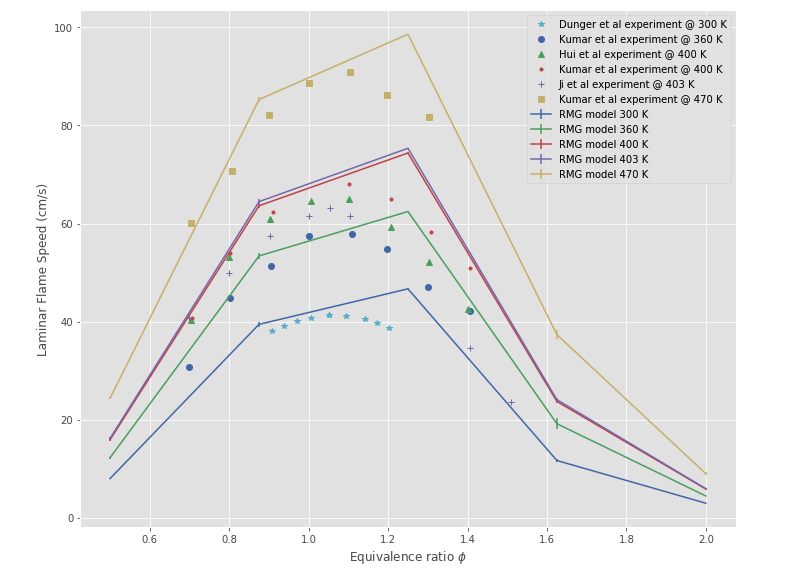
\includegraphics[scale=0.45, keepaspectratio]{images/nc10_flamespeeds.png}
    \caption{Premixed Laminar Flame Speeds of RMG n-decane/air mixtures at different temperatures of 300K, 400K, 403K, 470K at 1 atm against experiments of Wagner et al. \cite{Wagner1955FlameVelocity}, Kumar et al\cite{KUMAR2007209}, Hui et al. \cite{Hui2013LaminarPressures} and Ji et al \cite{Ji2010PropagationFlames}, lines represent RMG model prediction of current work, points represent experimental measurements}
    \label{fig:nc10_flamespeed}
    \end{small}
\end{figure}









\chapter{Iso-Octane Model}
\section{Kinetic Model}

Liquid transportation fuels are continuously used in different applications and the necessity to understand the reactivity of those fuels has been explored extensively in Chapter 1. Now we turn to the actual oxidation of the second primary reference fuel (PRF) of this work, which is iso-octane. Iso-octane is a member of the branched chain hydrocarbons with the functional group alkane (aliphatics). It is a symbolic name of one of the isomers of octane with the name 2,2,4-trimethyl-pentane using the IUPAC nomenclature alongside the Greek root word ``pent" meaning five but with 2-methyl groups on the second carbon and another methyl group on the fourth carbon atom. Thus, iso-octane is an 8-membered carbon atom with an iso-group branched hydrocarbon. The structure of iso-octane looked at in this work is of 2,2,4-trimethyl-pentane in the skeletal structure of fig.\ref{fig:iso-octane}. Iso-octane has the molecular formula of \ce{C_8H_18} since it is a member of the alkane family with a general structural formula of \ce{C_nH_{2n+2}}. 

\begin{figure}
    \centering
    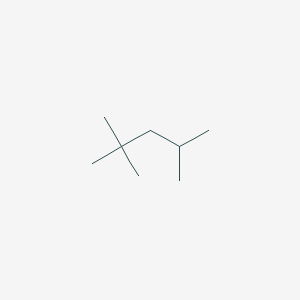
\includegraphics[scale=0.5, keepaspectratio]{images/2,2,4-Trimethylpentane_300.png}
    \caption{Iso-octane Structure}
    \label{fig:iso-octane}
\end{figure}

\vspace{2.5cm}


Iso-octane has long been identified as a constituent compound in the representation of transportation fuels \cite{Dooley2010AProperties}. Since it is representative of the important compounds in transportation fuels, enormous work has been done on the auto-ignition characteristics of the fuel. Experimental investigation of iso-octane includes ignition delay time measurements in shock tubes and rapid compression machines (RCM)  \cite{Fieweger1994Shock-tubePressures}\cite{Fieweger1997Self-ignitionPressure}\cite{Malewicki2013ExperimentalIso-octane}
\cite{Gauthier2004ShockMixtures}\cite{Hartmann2011Auto-ignitionModeling}, laminar flame speeds and flows \cite{BRADLEY1998126}\cite{KUMAR2007209}\cite{Li2012LaminarMixtures}\cite{Hui2013LaminarPressures}\cite{Bieleveld2009ExperimentalFlows}, chemical structure from pyrolysis and oxidation in pressure flow reactors \cite{Gokulakrishnan2007ExperimentalConditions}\cite{Jahangirian2012APressures}, oxidation and pyrolysis in shock tubes \cite{Malewicki2013ExperimentalIso-octane}\cite{Tekawade2016Time-resolvedN-dodecane} and oxidation in a jet stirred reactors \cite{Dagaut2015TheStudy}\cite{Dagaut2014CombustionModeling}\cite{Dagaut2008OxidationStudy}. These experimental measurements provide a basis with which to compare chemical kinetic models of iso-octane as means of validating the mechanisms. Similarly, several kinetic models of iso-octane have been published over the years with Ranzi et al \cite{Ranzi1997AOxidation}, publishing a semi-detailed model similar to n-heptane, Curran et al. \cite{Curran2002AOxidation}, showing the detailed low temperature and high temperature pathways, models have also been published on iso-octane using the CHEMKIN suite code from Malewicki et al \cite{Malewicki2013ExperimentalIso-octane}, iso-octane model has also been deduced based on surrogate modeling of jet aviation fuels using a three-component fuel surrogate model of n-decane, iso-octane toluene as described by Dooley et al \cite{Dooley2010MethylModel}. Westbrook et al \cite{Westbrook2009AN-hexadecane} published a combined model of \ce{C7} to \ce{C16}, Wang et al then constructed a very detailed model that integrates various fuels including n-alkane, cycloalkanes and alkyl-cycloalkanes in the JetSurF v2.0 model \cite{Wang2010A2.0},Sarathy et al followed up with a more compact model of \ce{C_7} to \ce{C_{20}} \cite{Sarathy2011ComprehensiveC20}.Although, skeletal models of iso-octane have been built in the past by Hartmann et al. \cite{Hartmann2011Auto-ignitionModeling}, based on the semi-detailed model of iso-octane and n-heptane Andrae et al. \cite{ANDRAE2008696} built. More recently, Atef et al \cite{Atef2017AKinetics} built a comprehensive iso-octane model with improved thermochemistry parameters and new isomerization pathways. All these iso-octane models built have been validated against various experimental conditions and there is still ongoing work to the determination of new pathways, reaction intermediates, better estimation of thermo-chemical parameters and rate constants for these kinetic models of iso-octane
. \par
\vspace{0.5cm}
The iso-octane model conditions as constructed in RMG have been outlined in Chapter 2 table \ref{tab:PRF_table1} as well as the reactor conditions used in table \ref{tab:PRF_table2} and table \ref{tab:PRF_table3}. This section is going to focus exclusively on the reaction pathways of iso-octane from high-temperature reaction to low-temperature as well as the flux diagram of fig. \ref{fig:f2} of the RMG model validated against published experiments with comparison to other published iso-octane kinetic models. The iso-octane model constructed in RMG was done on the basis of seed mechanisms of 
Burke et al\cite{Burke2012ComprehensiveCombustion}, Hashemi et al\cite{Hashemi2016High-pressureMethane} and Li et al\cite{Li2017TheoreticalC2H4} in the exact order as shown. The major reaction pathways shown in fig.\ref{fig:n-alkane-pathway} were discovered using the schematic and work of Merchant et al.\cite{Merchant2015UnderstandingPropane}, which used propane as a basis for the discovery of reaction pathways. As a result of this discovery, Merchant et al. concluded that the same scheme could be applied to n-alkanes and iso-alkanes up to \ce{C12} with an additional product of cyclic ethers from the \ce{QOOH} radical when they undergo cyclic ether formation reactions - where radicals move from one hydrogen to the other and a ring is formed as well as the loss of the \ce{OH} radical.



\newpage

\section{Reaction Pathways of Iso-octane Kinetic Model}
Iso-octane follows the class of reactions for its oxidation starting with a unimolecular fuel decomposition then a hydrogen abstraction reaction, and further down through a series of steps. H-abstraction reactions occur at both high and low temperatures. These class of reaction was proposed by Curran et al.\cite{Curran2002AOxidation} in the oxidation mechanism of iso-octane. At high temperatures, H-abstraction reactions occur via a $\beta$-scission - simply meaning that when the H-atom is removed, the radical is formed on the adjacent carbon atom to ensure thermodynamic stability and provide less steric hinderance to subsequent reacting species. Nonetheless, since at high temperatures, there is sufficient energy and collisions occur more rapidly, the radical though stable isomerizes and forms other radicals within the other akly groups of the radical atom with molecular formula \ce{C8H17}. The radical site varies depending on where the H-atom was removed. The easiest leaving sites are where the radical is stabilized by more substituted groups. Thus, radical sites that have a primary ($1^{\circ}$) H-atom are less favorable than those of the a secondary ($2^{\circ}$) H-atom and eventually a tertiary ($3^{\circ}$) H-atom. The radical sites with the most favorable H-atom abstractions are shown in fig.\ref{fig:ic8-radicalsites} leading to four distinct radicals of iso-octyl.
\begin{figure}[!htp]
    \centering
    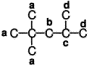
\includegraphics[keepaspectratio]{images/ic8-radical-sites.png}
    \caption{Radical sites for possible H-atom abstraction in iso-octane. Figure from \cite{Curran2002AOxidation}}
    \label{fig:ic8-radicalsites}
\end{figure}

These radicals eventually decompose further along the \ce{C-C} bonds and letting go of yet another hydrogen to form a double bond - olefins with another radical species, thus having a combination of
  \reaction{C-C-C^. \rightleftharpoons C=C + C}
This reaction family in RMG is represented as the R\textunderscore Addition\textunderscore MultipleBond.  Conversely, at low temperatures, the five decyl radicals first decompose again along the \ce{C-C} bond to form smaller alkyl radicals via the R\textunderscore Recombination reaction and these smaller alkyl radicals undergo reaction with \ce{O2} to form alkyl-peroxide radicals or \ce{ROO^.}. The various stages of the reactions are dependent on temperature, thus at higher temperatures the chain branching is not as complex, however at lower temperature many reaction pathways are possible. Since RMG has its own unique class of reaction families that assist in determining which reaction classes guide the fuel molecule to the products desired, we adopt Merchant et al.'s \cite{Merchant2015UnderstandingPropane} guide to following the oxidation of n-alkane and iso-octane fuels using the schematic of fig.\ref{fig:n-alkane-pathway} gives a pictorial illustration to find out the major reaction pathways of iso-octane, especially at low temperatures. In addition, since the onset of ignition in the Negative Temperature Coefficient (NTC) region is of interest, we use the illustration of Merchant et al.\cite{Merchant2015UnderstandingPropane} and Curran et al.\cite{Curran2002AOxidationc} to discover the pathways of low temperature reaction classes of iso-octane. The summary of the reaction classes as proposed by Curran et al.\cite{Curran2002AOxidation} and the corresponding RMG reaction families that enable the discovery of those pathways.





The major reaction classes for all the elementary reactions include the following:
\begin{enumerate}
    \item Unimolecular fuel decomposition
    \item H-atom abstraction from the fuel
    \item Alkyl radical decomposition
    \item Alkyl radical + \ce{O2} to produce olefin + \ce{HO2} radical directly
    \item Alkyl radical isomerization
    \item Abstraction reactions from olefin by OH, H, O and \ce{CH3}
    \item Addition of radical species to olefin 
    \item Alkenyl radical decomposition
    \item Olefin decomposition 
    \item Addition of alkyl radicals to \ce{O2} 
    \item Alkyl peroxy radical isomerization \ce{RO_2 \rightleftharpoons RO_2H}
    \item R\ce{O2^{.} + HO_2^.=RO_2H + O_2}
    \item R\ce{O_2^{.} + H2O2=RO2H + HO_2^.}
    \item R\ce{O2^{.} + CH3O2^{.}=RO^{.} + CH3O^{.} +O2}
    \item \ce{RO2^{.} + $R^\prime$O2^{.} = RO^{.} + $R^\prime$O^{.} + O2}
    \item \ce{RO2H=RO^{.} + O^{.}H}
    \item \ce{RO^.} decomposition
    \item \ce{Q^{.}OOH=QO+O^{.}H} cyclic ether formation via cyclization of diradical
    \item \ce{Q^{.}OOH}=olefin+\ce{HO2^{.}} (radical site $\beta$ to OOH group)
    \item \ce{Q^{.}OOH}=olefin + carbonyl + \ce{O^{.}H} (radical site $\gamma$ to OOH group)
    \item Addition of O2 to \ce{Q^{.}OOH}
    \item Isomerization of \ce{O2^{.}QOOH} and formation of ketohdroperoxide and \ce{O^{.}H}
    \item Decomposition of ketohydroperoxide to form oxygenated radical species and \ce{O^{.}H}
    \item Cyclic ether reactions with \ce{O^.H} and \ce{HO2^.}
\end{enumerate}
 
\begin{figure}
\hspace*{-3cm}
    \centering
    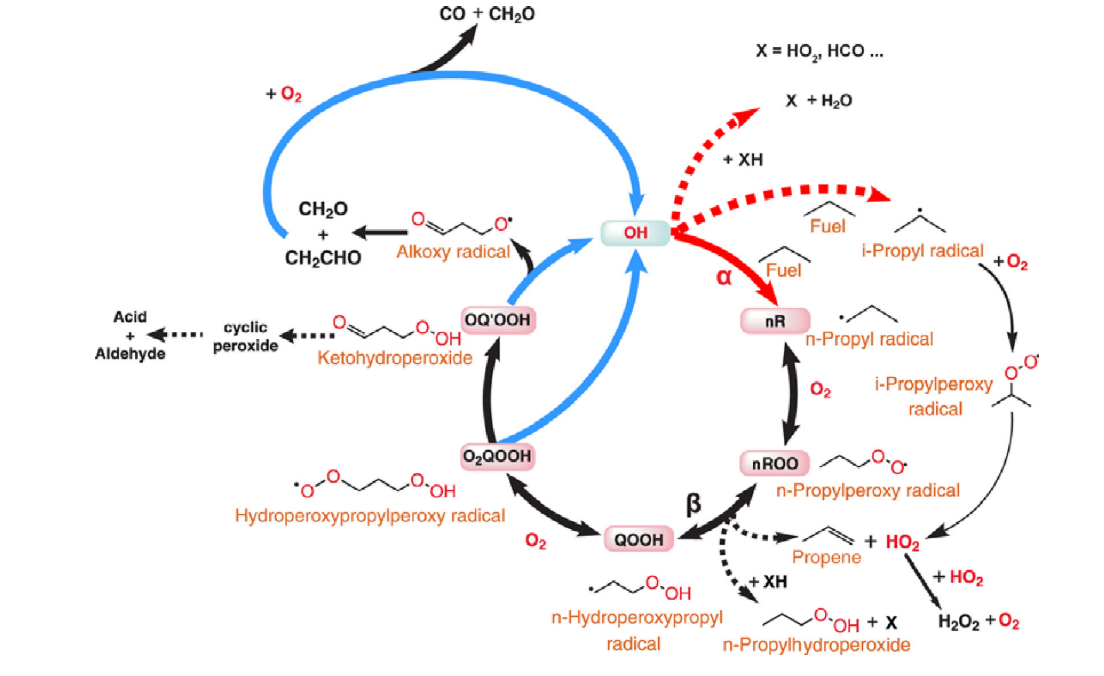
\includegraphics[scale=0.4, keepaspectratio]{images/rxn_class.png}
    \caption{Schematic of Merchant et al.\cite{Merchant2015UnderstandingPropane} major reaction pathways of propane during the first-stage of ignition. Reactions in blue lead to the formation of OH radicals. The reactions in dotted lines show competing pathways that divert radicals and lead to delay in the first-stage ignition}
    \label{fig:n-alkane-pathway}
\end{figure}

The convention of naming in this work is the R refers the the complete iso-octane mechanism while $R^\prime$ refers to the alkyl radical as seen in \ce{C^.}, Q refers to the isomerized form of \ce{ROO^.} via an intra H-migration reaction with molecular formula \ce{C_nH_{2n}}. For the reaction classes, the rates used are those from the reaction libraries as outlined in the summary of table \ref{tab:PRF_table1} and the seed mechanisms also outlined in table \ref{tab:PRF_table1}.

\cleardoublepage

\subsection{High Temperature Mechanism}

The high temperature mechanism can be accurately described with reaction classes 1-9.
\subsubsection{Unimolecular Fuel Decomposition and H-Abstraction Reactions} 
These reactions produce five alkyl radicals with the radical changing from one carbon atom to the next as well as an extra \ce{H} atom. Since the H atom abstraction reactions require high activation energies, they tend to favor the reverse direction as they serve as sink of H atoms. This initiation reactions are often observed in high temperature and pressure experiments such as that of shock tubes. In RMG, this reaction family is described by the H-Abstraction family with the general form 

\reaction{R^{1}-H^{2} + R^{3}\cdot \rightleftharpoons R^{1}\cdot {+} H^{2}-R^{3}\hspace{1cm} \text{H\textunderscore Abstraction reaction family}}

The four distinct iso-octyl radicals are show in fig.\ref{fig:iso-octyl_radicals}

\begin{figure}[!htp]
    \centering
    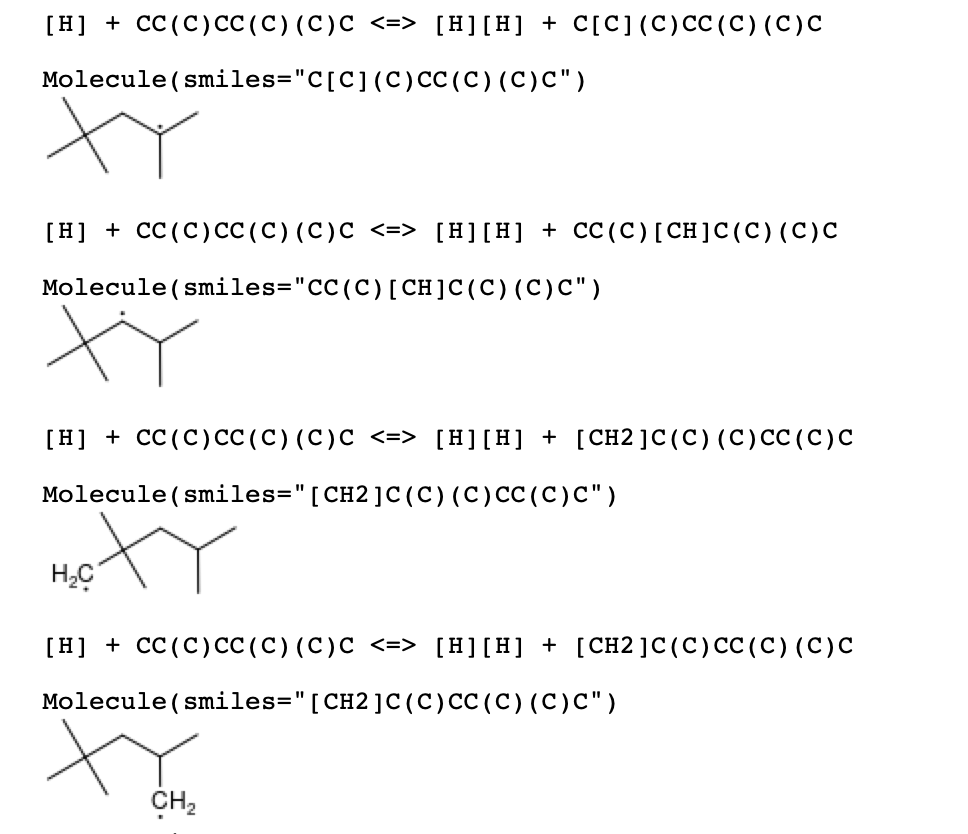
\includegraphics[keepaspectratio]{images/iso-octyl-radicals.png}
    \caption{Iso-octyl radicals from the H-atom abstraction}
    \label{fig:iso-octyl_radicals}
\end{figure}

\subsubsection{Alkyl Radical Decomposition Reactions}
Alkyl radical decomposition reactions involve the breaking of the previously generated alkyl radical along the C-C bonds and is only relevant at high temperatures $>$ 850 K \cite{Curran1998AOxidation}. There is competition usually between this reation pathway and the addition of \ce{O2} to the alkyl radicals because of the low energy barrier for the addition of \ce{O2}, the pathway to give ROO can sometimes be favored. However, for larger alkanes > C8 the breaknig of the alkyl radical usually occurs via the $\beta$-scission to aid for the addition of the \ce{O2}. This reaction often leads to the formation of olefins (alkenes) or C=C double bonds as well as another radical. This reaction family is described in the RMG reaction family as radical recombination as the breaking down of the C-C bond usually favors the reverse direction with a general form as this 

\reaction{{R^{1}\cdot {+} R^{2}\cdot \rightleftharpoons R^{1}-R^{2}} \hspace{1cm} \text{R\textunderscore Recombination reaction family}}

\subsubsection{Alkyl Radical + \ce{O2} = Olefin + \ce{HO2^{.}} and Alkyl Radical Isomerization Reactions}

The reaction of alkyl radicals with \ce{O2} can undergo through various reaction paths. The reaction channel usually involves the addition of \ce{O2} in the form of \ce{O^{.}-O^.} where Oxygen is represented as a biradical singlet since this is the most stable form in its electronic structure. This reaction adds to the alkyl radical via the radical recombination channel and forms a alkylperoxy radical which then undergoes an isomerization to form a hydroperoxy-alkyl radical with the loss of a hydrogen atom. This new form is often labeled as \ce{QOOH} where the Q usually denotes the presence of a double bond. The reaction family of the first step from alkylperoxy radical to hydroperoxy-alkyl radical is the intra\textunderscore H\textunderscore migration and then finally to form the double bonded olefin is the R\textunderscore Addition\textunderscore MultipleBond.

\reaction{{H^{3}-R^{2}\thicksim R^{1}\cdot \rightleftharpoons R^{2}\cdot\thicksim R^{1}-H^{3}} \hspace{1cm} \text{intra\textunderscore H\textunderscore migration reaction family}} 
\reaction{R^{2}=R^{1} + R^{3}. \rightleftharpoons R^{2}.-R^{1}-R^{3}\hspace{1cm} \text{R\textunderscore Addition\textunderscore MultipleBond reaction family}}

The \ce{ROO^.} radicals are shown in fig.\ref{fig:iso-octyl-peroxy radicals} when \ce{O2} is added to the iso-octyl radicals and during the inner H-atom migration process isomerizes to the iso-octyl-hydroperoxy radicals \ce{Q^{.}OOH} shown in fig.\ref{fig:ic8-QOOH}.

\begin{figure}[!htp]
    \centering
    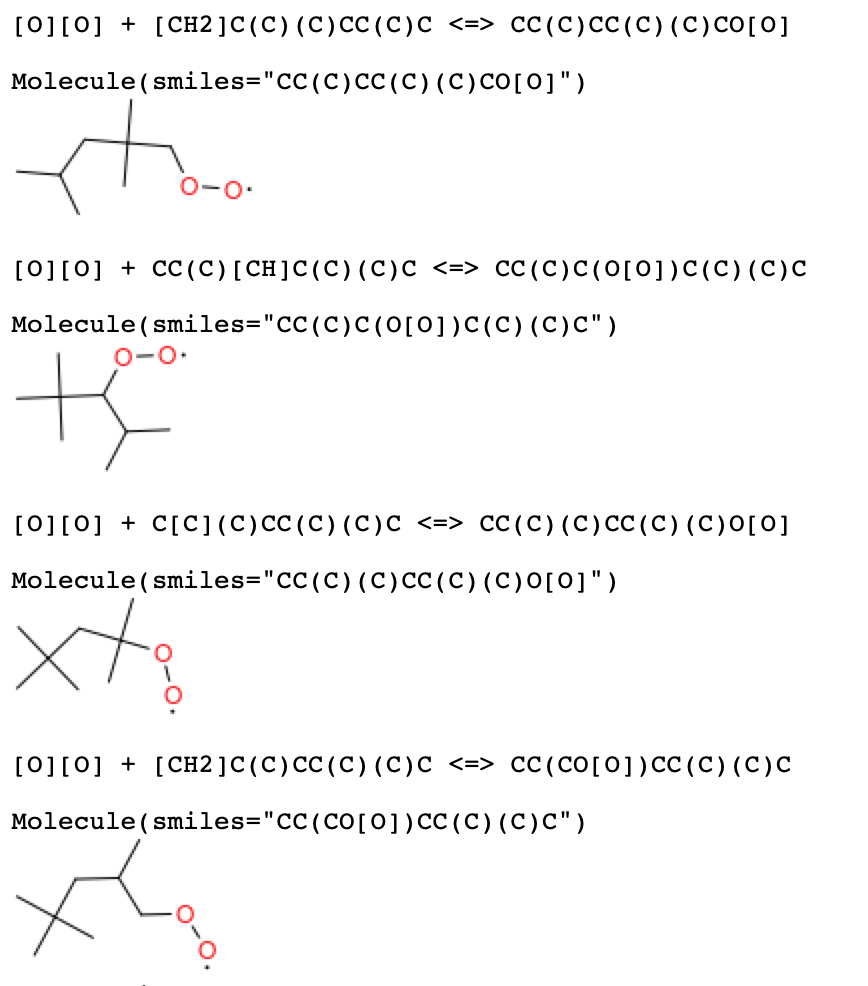
\includegraphics[scale=0.45, keepaspectratio]{images/iso-octyl-ROO.png}
    \caption{Iso-octylperoxy radicals }
    \label{fig:iso-octyl-peroxy radicals}
\end{figure}

\begin{figure}[!hbp]
    \centering
    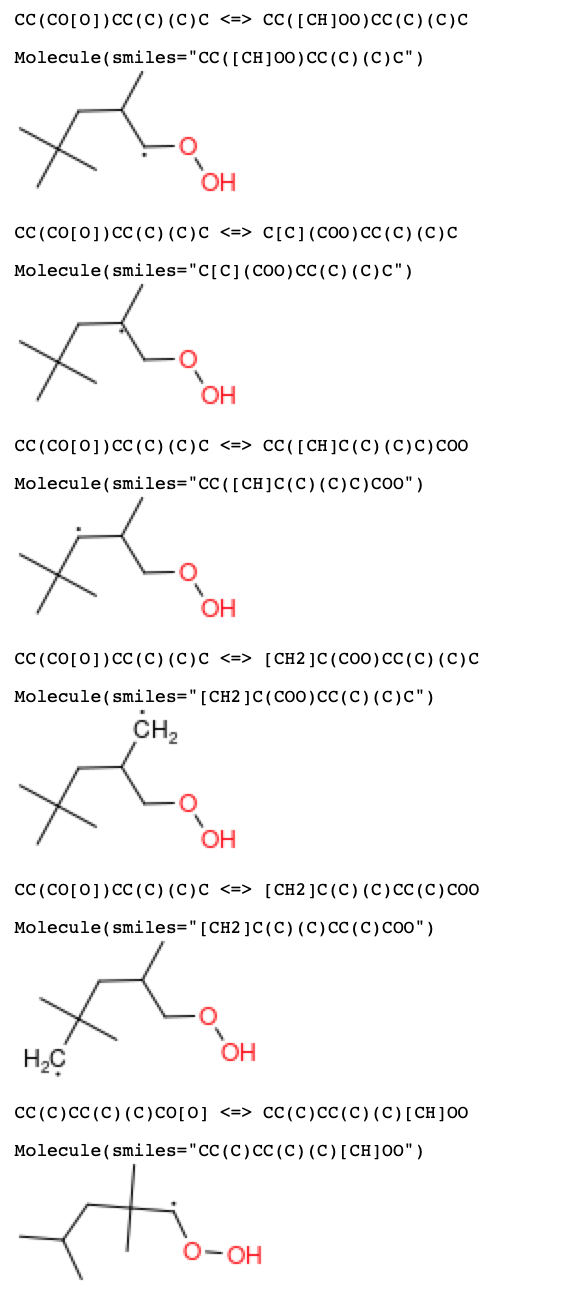
\includegraphics[scale=0.45, keepaspectratio]{images/iso-octyl-QOOH.png}
    \caption{Iso-octyl-hyrdoperoxy radicals \ce{Q^{.}OOH}}
    \label{fig:ic8-QOOH}
\end{figure}

Reaction classes 4-9 deal entirely with reactions of olefins. Since at high temperatures, the steric considerations are complex in the reaction channels, more emphasis is left on this reactions as the rate expressions are very complex in describing the pathways.
\newpage
\subsection{Low Temperature Mechanism}
The low temperature mechanism can be described as reactions at temperatures $<$ 900 K with reaction classes 10-24.

\subsubsection{Addition of alkyl radicals to \ce{O2} and Alkyl peroxy radical isomerization \ce{RO2 \rightleftharpoons RO2H}}

The $\beta$-scission high activation energies makes reactions much slower, thus reactions with lower activation energies take precedence. The first is the addition of oxygen \ce{O2} to the alkyl radical and then isomerization reactions on the ROO radicals occur throughout the radical moving the radical sites with a \ce{H}-atom shift (internal H-abstraction) on the radical. 
\reaction{H^{3}-R^{2}\thicksim R^{1}\cdot \rightleftharpoons R^{2}\cdot\thicksim R^{1}-H^{3} \hspace{1cm} \text{intra\textunderscore H\textunderscore migration reaction family}} However, these internal H-abstraction reactions (H-migrations) are rather slow at lower temperatures thus making the addition of ROO decomposition to yield two reactive reactive hydroxyl radical and a carbonyl group. Evidently, Pollard \cite{Pollard1977Hydrocarbons} carried out extensive low temperature kinetic analysis of hydrocarbon oxidations and mapped out the most important features of low temperature submechanism. Many recent models have integrated these features in their models for simplifications essential for the oxidation of low temperature hydrocarbons. 



\subsubsection{Radical decomposition of \ce{RO2H \rightleftharpoons RO^{.} + O^{.}H} and \ce{Q^{.}OOH \rightleftharpoons QO + O^{.}H} }
The first step of the decomposition of \ce{RO2H} alkyl-hydroperoxides is one of the very important steps in the process of hydrocarbons and often controls the onset of a Negative temperature coefficent (NTC) regime in the auto-ignition of hydrocarbons. Thus, the production of the \ce{O^{.}H} radicals is necessary for the first-stage ignition process \cite{Merchant2015UnderstandingPropane} as well as the optimization process for cetane sensitizer improvements \cite{Curran1998AOxidation}. In order to form the alkenyl-hydroperoxy radicals \ce{Q^{.}OOH} from the alkyl-peroxides \ce{RO2}, unimolecular isomerizations occur again via the intra\textunderscore H\textunderscore migration reactions. 

When the alkoxy radicals are produced \ce{RO^.} from the decomposition of the alkyl-hydroperoxides \ce{RO2H}, they often tend to be unstable and decompose more readily to the stable form of oxygenated alkoxy radicals for large carbon chains often $>$ C8 with the presence of carbonyl groups such as aldehydes and ketones and other smaller alkoxy radical species via the intra\textunderscore H\textunderscore migration reaction family. The smaller alkyl radicals decompose even further eventually following a $\beta$-scission to form olefins (alkenes) via the R\textunderscore Addition\textunderscore MultipleBond reaction family, which is stable in this form by the presence of its pi bonds. For the aldehydes, due to the presence of a double bonded oxygen, they are reactive and additions to the double bond are possible forming yet another alkyl radical and another oxygen radical which can attack double bonds. 


As the radical decomposition continues, the alkenyl-hyrdoperoxy radicals involves the breaking of the \ce{O-O} bond with the chain branching to form cyclic ethers with an extra \ce{O} atom in the chain.As the chain branching begins, cyclic ethers are formed with the loss of the internal \ce{H} from QOOH as a competing reaction pathway. The cyclic ether formation has a unique reaction family in the RMG database that forms from the \ce{QOOH} radical seen as \reaction{R^{1}^.\thicksim O^{2}-O^{3}-R  \rightleftharpoons R^{1}\thicksim O^{2} + O^{3}R^. \hspace{1cm} \text{Cyclic\textunderscore Ether\textunderscore Formation }} The presence of these cyclic ethers is shown in the schematic of Merchant et al.\cite{Merchant2015UnderstandingPropane} fig.\ref{fig:cyclic-ethers}. 

\begin{figure}[!ht]
\hspace*{-3cm}
    \centering
    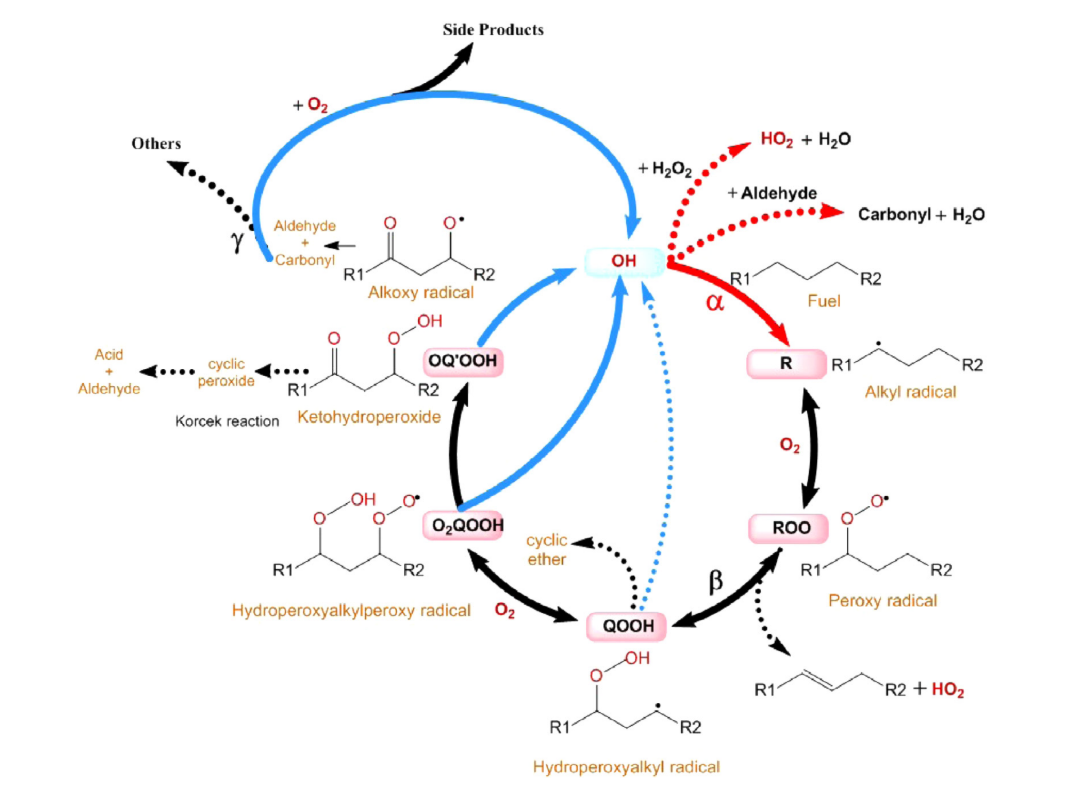
\includegraphics[scale=0.45, keepaspectratio]{images/nalkane-schematic+ROR.png}
    \caption{Schematic of low temperature oxidation of n-alkanes with the presence of cyclic ethers as shown by Curran et al.\cite{Curran1998AOxidation} and schematic from Merchant et al.\cite{Merchant2015UnderstandingPropane}}
    \label{fig:cyclic-ethers}
\end{figure}


\subsubsection{Decomposition of \ce{Q^{.}OOH \rightleftharpoons Olefin + HO2^.} and \ce{Q^{.}OOH \rightleftharpoons Olefin + Carbonyl + O^{.}H}}

Alkenyl-hydroperoxide radicals \ce{Q^{.}OOH} have a $\beta$ radical site that can decompose to an olefin and hydroperoxy radical \ce{HO2^{.}} via an addition reaction along the \ce{Q-OOH} site. The \ce{HO2^.} radicals often play an important role in the auto-ignition process of hydrocarbons and contributes to the NTC behavior of n-decane. Similarly, rather than decomposition along the \ce{Q-OOH} site, $\beta$-scission can occur and the presence of olefins alongside a smaller carbonyl group usually a ketone and a hydroxy radical \ce{O^.H} is formed. These three body reactions usually have very high weak dependence on temperature and its rate estimates are often observed to be very close to the high pressure limit and violate the collision limits of the Lennard-Jones parameter as described by Chen et al.\cite{Chen2017ViolationModels}. 


\subsubsection{Addition of \ce{O2} to \ce{Q^.OOH} and Isomerization of \ce{O2^.QOOH} to Ketohydroperoxide and \ce{O^.H} radicals}
Alkenyl-hydroperoxide \ce{Q^.OOH} radicals can react with \ce{O2} via radical recombination reactions to form peroxy alkenyl-hydroperoxide radicals \ce{O2^.QOOH}. \reaction{R^{1}\cdot {+} R^{2}\cdot \rightleftharpoons R^{1}-R^{2} \hspace{1cm} \text{R\textunderscore Recombination reaction family}}
 
 Further chain branching steps of the peroxy-alkenyl-hydroperoxide radicals can form \ce{HOOQ^.OOH} dihydroperoxy-alkenyl radicals via an inernal H migration reaction before the final isomerization reaction to eliminate the \ce{O^.H} radicals and form different ketohyperoxide species depending on the carbon chain. The QOOH radicals alongside chain branching form a combination of carbonyl groups of ketones and olefins as well as OH radicals. The \ce{O2QOOH} species then isomerize to form ketohydroperoxides and OH radicals along the double bonds.  
 
 The full pathways integrating both the high and low temperature chemistry is seen in fig.\ref{fig:f2} of n-decane.

\begin{figure}[!htp]
    \centering
\hspace*{-3cm}
    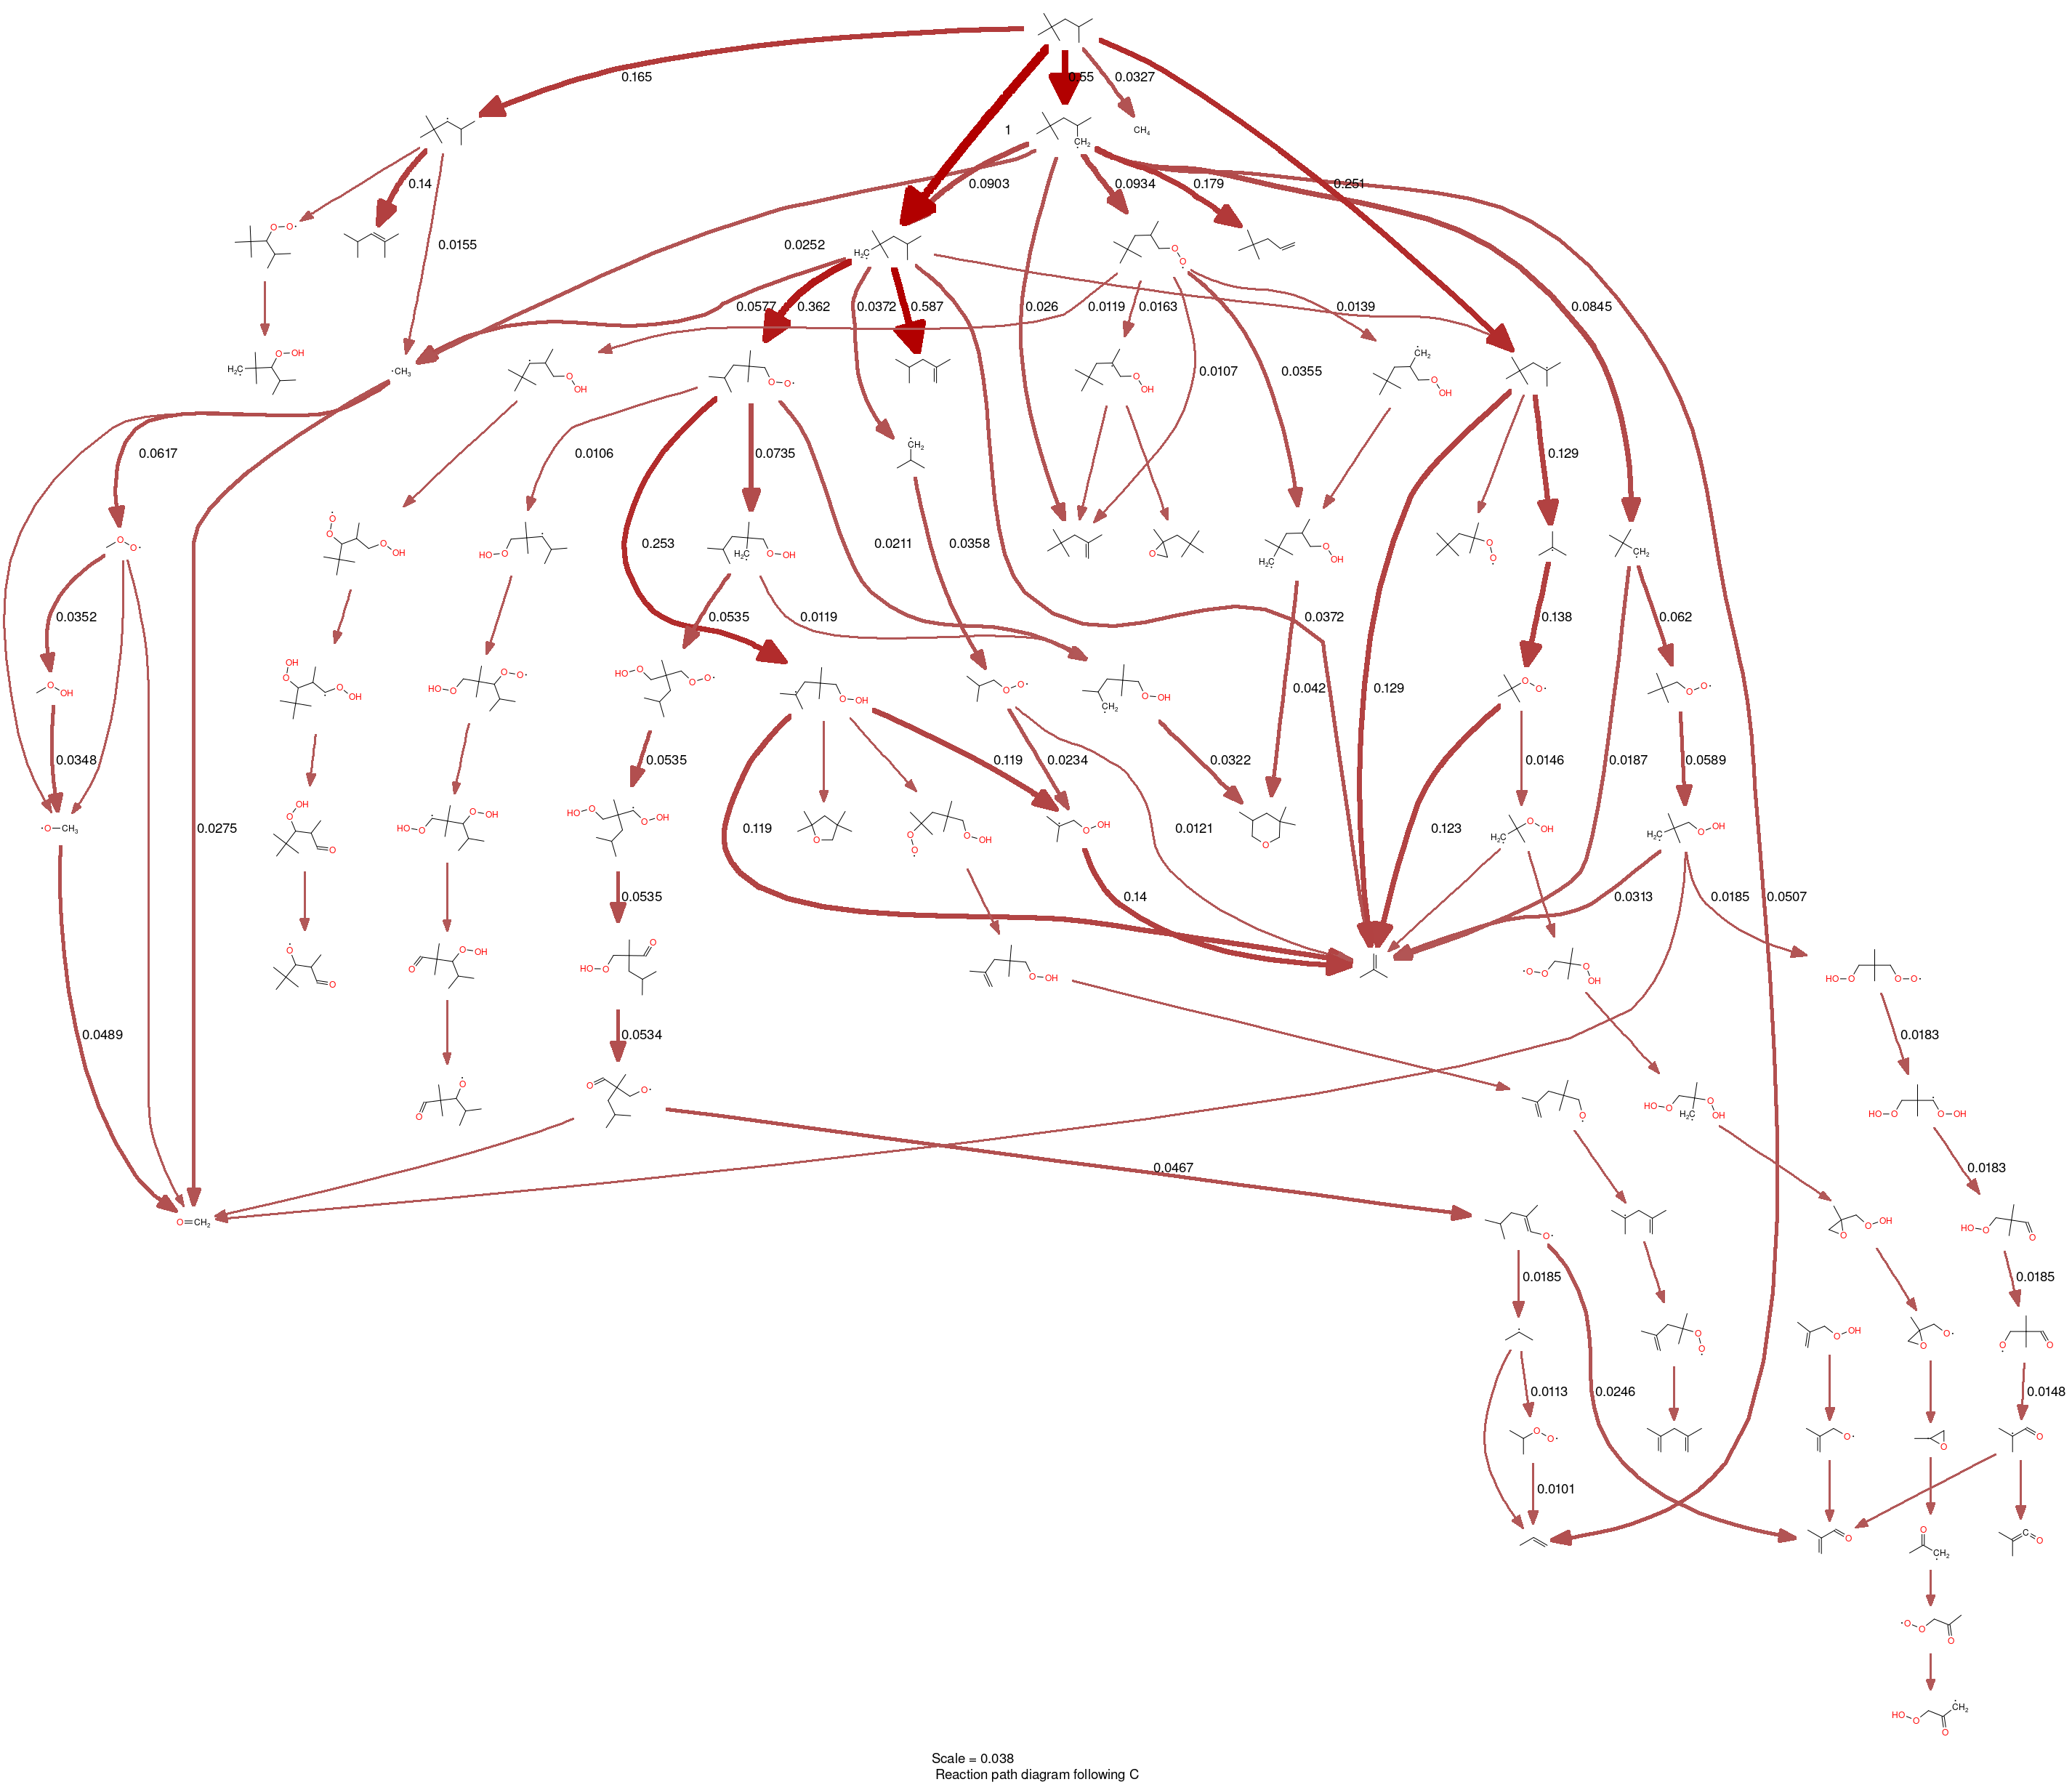
\includegraphics[scale=0.2,keepaspectratio]{images/ic8-flux_pathways.png}
    \caption{Flux diagram of iso-octane @ 800K and 13 bar}
    \label{fig:f2}
\end{figure}

\cleardoublepage

\section{Model validation of iso-octane under experimental conditions}
The detail of the model generation of iso-octane using RMG has been described in sufficient detail with the inclusion of both the high temperature and low temperature reaction pathways as well as the model generation process algorithm highlighted in Chapter 2. Now we look into the validation of the iso-octane model using the chemical kinetics code Cantera \cite{cantera}. The model is only validated against experiments of Shock Tubes for ignition delay time measurements at a wide range of conditions.


\subsection{Model validation of iso-octane in shock tubes for ignition delay time predictions}
Shock tubes essentially devices designed to experiment and study the flow of high-temperature and high-velocity effects of compressible gases within an actual engine-like environment. It is designed on the basis of knowledge of gas dynamics and analysing shock waves. It operates on the principle that at high temperatures, supersonic gases flow is in the tube a diaphragm causes a separation into regions of high-pressure and low-pressure. As the pressure rises, an unsteady rarefied wave passes into the driver gas with a velocity usually a few kilometers per second causing flow from the high-pressure region to the low-pressure region. As the shock wave progresses in the low-pressure region, it pushes the low-pressure gas ahead of it. Thus, creating two fronts, flow ahead of the shock wave and flow behind the shock wave. The flow ahead of the behind the shock wave (driver gas) is the gas of interest. The velocity of the driver gas is equal to  that of the driven gas\cite{Greene1964TheR.}. Usually, there in the high-pressure region, is an explosive gas which is the gas studied, and present is a laser beam to detect the luminescence of some excited species. The ignition delay time can be defined as the time it takes:
\begin{enumerate}
    \item For the shock wave to hit the wall and propagate with the excitation of a \ce{CH*} or \ce{OH*}radical
    \item For the shock wave to hit the wall and measurement of the highest peak of the temperature in the driven section
    \item For the shock wave to hit the wall and detection of the highest peak of the pressure in the driven section
\end{enumerate}
Since all three possibilities of measuring the ignition delay time data in shock tubes exist, it is often well defined based on one of the three main possibilities usually for the first-stage ignition \cite{Davidson2004InterpretingData}\cite{Fieweger1994Shock-tubePressures}\cite{Fieweger1997Self-ignitionPressure}\cite{Pfahl1996Self-ignitionConditions}\cite{Haylett2012IgnitionTube}

In Cantera, this process is often defined based on the reactor type of interest. First, the gas solution object is created with the \textbf{gas.Solution} class, then a reactor type is selected with the appropriate initial conditions usually coming from the experimental data being validated against. Next, the state of the system is set with the reactor network previously defined and then a simulation in time for the next states is found using the ODE solver. The ODE solver starts at the current state  of the systems and progresses in time by one of the following methods:
\begin{enumerate}
    \item \textbf{step()}: This involves a reactor step from the current state of the system by solving the previous state of the system using the time step given. This is an explicit method where the ODE solver internally solves the numerical Differential Algebraic Equations (DAE) system. The new time is returned as well as the state of the system at the next state using the previously defined time step $\Delta$t within the solver absolute and relative tolerances. The time step cannot be larger than the maximum time step or else the ODE solver breaks.
    \item \textbf{advance($t_{new}$)}: This method solves the state of the system at a predefined step times $t_{new}$. This $t_{new}$ describes the absolute time of the system from the initial system by calling the ignition delay time function for the reactor in a loop, either a while loop or for loop at exactly the time specified - basically using the \textbf{step():} function several times in the process. In addition, the \textbf{advance():} function can be made to continue until a steady-state solution is attained by time stepping. Only when the feature-scaled residual of the state vector is below a given threshold value is the system at steady-state and the ODE solver stops.
\end{enumerate} 
For all shock tube models in this work, a zero-dimensional homogeneous closed ideal gas reactor with constant volume and internal energy class was used since at constant volume, there is no P-V work done against the control volume of the gas. Since the temperature is known, the energy equation is computed assuming adiabatic conditions in the reactor volume. The time integration of the species is computed in uniform time steps until the solution is found. During the time integration, the reactor model scheme usually an ODE SUNDIALS solver \cite{hindmarsh2005sundials} solves the differential equations of the species within the energy equation. The energy equation accounts for the energy interaction via the heat equation but is ignored since the reactor assumes adiabatic conditions and indicates only mechanical work interactions, mass transport due to species diffusion and conversion.  The equation being solved in the ideal gas reactor  of Cantera is equation \ref{eq.mass conservation} as given by Robert Kee et al's book on Chemically Reacting Flow \cite{Kee2003ChemicallyPractice}. The definition of the ignition delay time varies. Nonetheless, the model used in Cantera assumes an ignition delay time based on the excited \ce{CH} or \ce{OH} radical species and is often very close to the highest temperature spike Ji et al point out for the sensitivity analysis of ignition delay times \cite{Ji2019EvolutionAutoignition}. 

\begin{equation}
    U = m\sum_k{Y_k u_k(T)}
\end{equation}

\begin{equation}
    \frac{dU}{dt} = u\frac{dm}{dt}+mc_v\frac{dT}{dt}+m\sum_k{u_k \frac{dY_k}{dt}}
\end{equation}

\[\text{Substituting the corresponding derivations for temperature in the reactor as:} \]


\begin{equation}
    mc_v\frac{dT}{dt}=-p\frac{dV}{dt} - Q^. + \sum_{in}{m_{in}(h_{in}- \sum_k{u_k Y_{k, in}}) -\frac{pV}{m}\sum_{out}{m_{out}^.} - \sum_k{m_{k, gen}^. u_k}}
    \label{eq.mass conservation}
\end{equation}

The ignition delay times prediction are presented as modeled in Cantera against shock tube experiments of Fieweger et al.\cite{Fieweger1994Shock-tubePressures}\cite{Fieweger1997Self-ignitionPressure} in fig.\ref{fig:idt times}.

As seen in fig. \ref{fig:idt times}, there is good agreement between the model prediction of ignition delay times against the experiments of Fiewger et al. who studied the self-ignition of several spark-ignition (SI) engine fuels between lean, stoichiometric and rich fuel mixtures under engine-like conditions in a high pressure shock tube and observed a transition from deflagration-like behavior to a  detonation-like behavior around 960 K with strong high pressure peaks, cool flame and onset of a NTC regime in a two-step ignition.


\begin{figure}[!hbp]
    \centering
    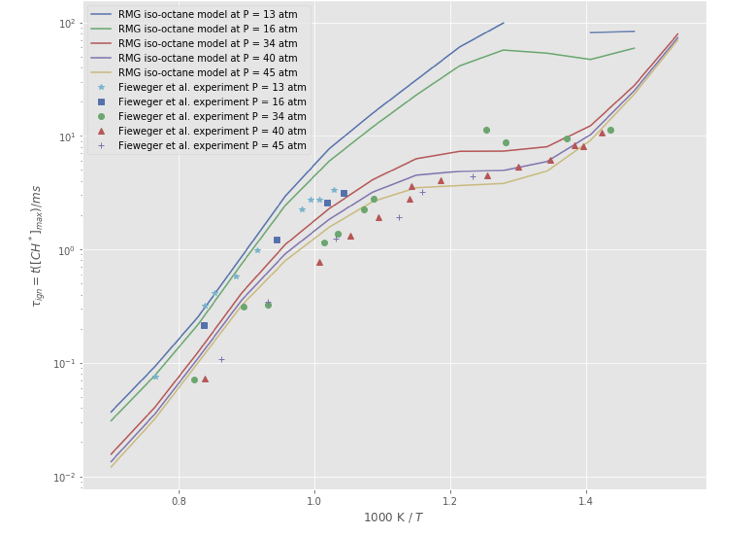
\includegraphics[scale=0.4, keepaspectratio]{images/ic8-idt.png}
    \caption{Ignition delay time prediction of iso-octane/air at 13 atm, 16 atm, 34 atm, 40 atm and 45 atm for $\phi=1$ stoichiometric mixtures against experiments of Fieweger et al. \cite{Fieweger1994Shock-tubePressures}\cite{Fieweger1997Self-ignitionPressure}. Lines indicate model predictions and symbols indicate experiments}
    \label{fig:ic8-idt}
\end{figure}

\cleardoublepage
\subsubsection{Sensitivity Analysis of the Ignition delay times}
A detailed analysis was done to determine which control variables control the ignition delay of the iso-octane model. Since the species usually measured for the onset of ignition is the \ce{OH^.} radical \cite{Ji2019EvolutionAutoignition}, the concentration of the \ce{OH^.} radical was used as the criteria for sensitivity by the use of a brute force method comparing the localised sensitivity at a given temperature for all the top 20 most sensitive reactions that influence the ignition delay time. This sensitivity analysis was done at high temperatures of 1300 K, intermediate temperatures of 900K and at low temperatures of 700K to observe which reactions contribute the most to either the production or consumption of the \ce{OH^.} radical species. 

The sensitivity analysis involves the perturbation of both the forward and reverse rates of the 20 most sensitive reactions to \ce{OH^.} radical concentration by a factor of two and then comparing the change in the ignition delay time to the preset (original )rate constant of those same reaction ignition delay time sensitivity coefficients to the \ce{OH^.} radical species. The magnitude of the sensitivity coefficient indicates a strong dependence on \ce{OH^.} radical concentration, while the sign indicates rate of production if positive and rate of consumption if negative. The sensitivity plots are shown in fig.\ref{fig:ic8-sensitivity}.

The summary of the RMG iso-octane model is given in table \ref{tab:iso-octane_model_summary}. 
\begin{table}[ht]
\arrayrulecolor[HTML]{DB5800}
\caption{Summary of RMG iso-octane model analysis and Ignition delay time prediction at extinction }
\centering
\begin{adjustbox}{width=1\textwidth}
\begin{tabular}{ p{6cm} c c c c }
\rowcolor{lightgray}\multicolumn{4}{|c|}{RMG iso-octane model summary} \\
Number of Species before sensitivity analysis & 492 & &  \\ 
Number of species after sensitivity analysis  & 19558 & &  \\
Number of Reactions before Sensitivity analysis & 19558 & & \\ 
Number of reactions after sensitivity analysis & 19558 & & \\ 
\hline
 Model ignition delay time at extinction &  Temperature & Pressure & Equivalence ratio \\
 \begin{tabular}{ c }
    $\tau$=98.6775 ms   \\
    $\tau$=59.17276 ms \\ 
    $\tau$=78.6791 ms \\
    $\tau$=73.26734 ms \\
    $\tau$=69.76976 ms \\ 
 \end{tabular} & \begin{tabular}{ c } 
       782.1229 K\\
      679.6116 K \\
      651.16279 K \\
     651.16279 K \\
     651.16279 K \\
 \end{tabular} & \begin{tabular}{ c }
      13 bar  \\
      16 bar \\
      34 bar \\
      40 bar \\
      45 bar \\
 \end{tabular} & 1.0 \\
 \end{tabular}
    \end{adjustbox}
    \label{tab:iso-octane_model_summary}
\end{table}


\begin{figure}
    \centering
    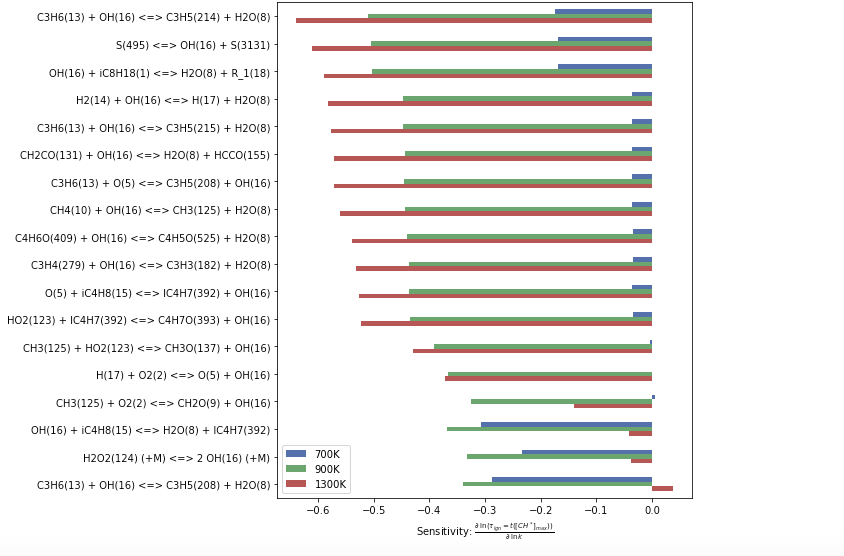
\includegraphics[scale=0.45, keepaspectratio]{images/sensitivity-iso-octane.png}
    \caption{Sensitivity coefficients of the ignition delay time of the iso-decane model to \ce{OH^.} radical concentration at stoichiometric fuel/air mixture at 700 K, 900 K, 1300 K at $P=13$ bar. Where the ignition delay times $\tau_{ign}=t(\ce{CH^.}_{max})$}
    \label{fig:ic8-sensitivity}
\end{figure}


\begin{figure}
    \centering
    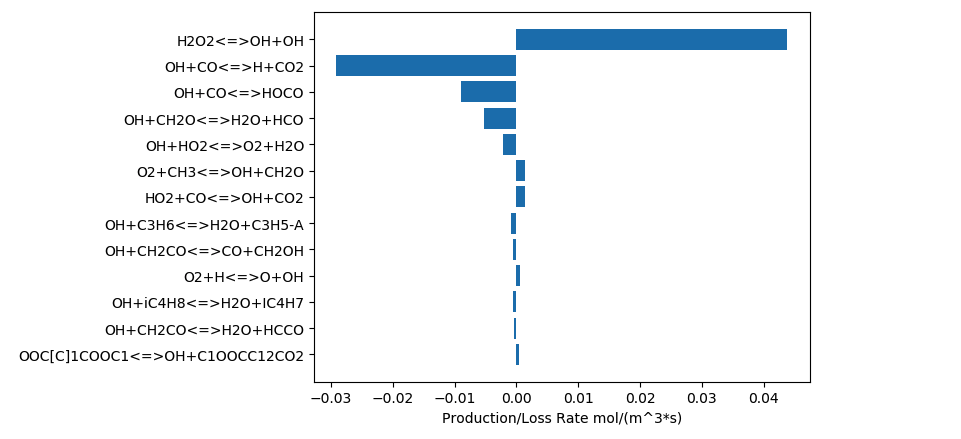
\includegraphics[scale=0.45, keepaspectratio]{images/ic8-ROP.png}
    \caption{Rates of Production/Consumption of the \ce{OH^.} radicals of the iso-octane model}
    \label{fig:rop-nc10}
\end{figure}
\chapter{N-propyl-cyclohexane (PCH) Model}
\section{Kinetic Model}

Liquid transportation fuels are continuously used in different applications and the necessity to understand the reactivity of those fuels has been explored extensively in Chapter 1. Now we turn to the actual oxidation of the second primary reference fuel (PRF) of this work, which is n-propyl-cyclohexane. N-propyl-cyclohexane is a member of the straight chain cycloalkane hydrocarbons commonly called naphthenes. Naphthenes are usually present in liquid transportation fuels adequate knowledge of their combustion properties is of great interest in the design of Homogeneous Charge Compression Ignition (HCCI) engines as alternatives to spark ignition (SI) engines. While this study has been applied to large and heavy duty machinery, naphthenes play an important role in the overall composition of liquid transportation fuels as well as the design and optimization of HCCI engines \cite{Aceves1999CompressionCombustion}. Although, alkanes both straight chain and branched chain alkanes dominate the composition of liquid transportation fuels with 80\% - 90\% being either n-decane, n-dodecane for straight chain reference fuel composition and iso-octane as a model fuel for branched alkanes , common naphthenes found in transportation fuels include cyclohexane, alkyl-cyclohexane from methyl-cyclohexane, ethyl-cyclohexane and up to n-butyl-cyclohexane \cite{Granata2003ANaphthenes}. 

The structure of n-propyl-cyclohexane looked at in this work is the straight chain propyl-cyclohexane in the skeletal structure of fig.\ref{fig:n-pch}. N-propyl-cyclohexane has the molecular formula of \ce{C_9H_18} since it is a member of the cycloalkane family with a general structural formula of \ce{C_nH_{2n}}. 

\begin{figure}[!htp]
    \centering
    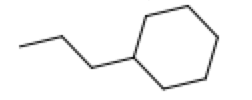
\includegraphics[scale=0.5, keepaspectratio]{images/pch-skeletal-formula.png}
    \caption{n-propyl-cyclohexane Structure}
    \label{fig:n-pch}
\end{figure}




N-propyl-cyclohexane has long been identified as a constituent compound in the representation of transportation fuels \cite{Pousse2010LeanN-Propylcyclohexane}. Since it is representative of the important compounds in transportation fuels, enormous work has been done on the auto-ignition characteristics of the fuel. Experimental investigation of n-propyl-cyclohexane includes ignition delay time measurements in shock tubes and rapid compression machines (RCM)  \cite{Dubois2009ExperimentalConditions}\cite{Crochet2010AConditions}\cite{Tian2014ComparativeN-Propylcyclohexane}, laminar flame speeds \cite{Pousse2010LeanN-Propylcyclohexane}\cite{Crochet2010AConditions}, chemical structure from pyrolysis and oxidation in pressure flow reactors and jet stirred reactors \cite{Bales-Gueret1992ExperimentalReactor} \cite{Ristori2001TheModeling}\cite{Dagaut2015TheStudy}\cite{Dagaut2014}\cite{Dagaut2016ExperimentalSurrogates}\cite{Gokulakrishnan2008IgnitionFuel}\cite{Gokulakrishnan2007ExperimentalConditions}. These experimental measurements provide a basis with which to compare chemical kinetic models of n-propyl-cyclohexane as means of validating the mechanisms. Similarly, several kinetic models of n-propyl-cyclohexane have been published over the years using the chemical kinetic mechanism generation code EXGAS \cite{Warth2000ComputerOxidation} used by Battin-Leclerc and others \cite{Battin-Leclerc2008DetailedSurrogates}, models have also been published on n-propyl-cyclohexane using the CHEMKIN suite code from Dubois et al \cite{Dubois2009ExperimentalConditions}, n-propyl-cyclohexane model has also been deduced based on surrogate modeling of jet fuels using a biokerosene fuel surrogate model of n-hexadecane, n-propylcyclohexane, n-propylbenzene and n-decane as described by Dagaut et al \cite{Dagaut2007ChemicalCombustion} as well as the synthetic diesel fuel surrogate model of Mati et al.\cite{Mati2007TheModeling} that consisted of n-hexadecane(36.1\% by weight, 23.5\% vol.), n-propylcyclohexane (23.1\% weight, 26.9\% vol.), n-propylbenzene (18.7\% weight, 22.9\% vol.), iso-octane(14.7\% weight, 19\% vol.) and 1-methylnaphthalene (7.4\% weight, 7.7\% vol.). Westbrook et al \cite{Westbrook2009AN-hexadecane} published a combined model of n-octane to n-hexadecane, Wang et al then constructed a very detailed model that integrates various fuels including n-alkane, cycloalkanes and alkyl-cycloalkanes in the JetSurF v2.0 model \cite{Wang2010A2.0}.Although, submechnanisms and skeletal models of n-propyl-cyclohexane have been built in the past by Ristori et al \cite{Ristori2001TheModeling}, more recently, Abbasi et al \cite{Abbasi2018KineticFormation} built a submechanism for n-propyl-cyclohexane coupled with new pathways for polycyclic aromatic hydrocarbons (PAH) formation. All these n-propyl-cyclo-hexane models built have been validated against various experimental conditions and there is still ongoing work to the determination of new pathways, reaction intermediates, better estimation of thermo-chemical parameters and rate constants for these kinetic models. \par
\vspace{0.5cm}
The n-propyl-cyclohexane model conditions as constructed in RMG have been outlined in Chapter 2 table \ref{tab:PRF_table1} as well as the reactor conditions used in table \ref{tab:PRF_table2} and table \ref{tab:PRF_table3}. This section is going to focus exclusively on the reaction pathways of n-propyl-cyclohexane, only the high-temperature reaction mechanism as well as the flux diagram of fig. \ref{fig:f2} of the RMG model validated against published experiments with comparison to other published n-propyl-cyclohexane kinetic models. The n-propyl-cyclohexane model constructed in RMG was done on the basis of seed mechanisms of 
Burke et al\cite{Burke2012ComprehensiveCombustion}, Hashemi et al\cite{Hashemi2016High-pressureMethane} and Li et al\cite{Li2017TheoreticalC2H4} in the exact order as shown. 

The reaction library used ``violator\textunderscore fixes\textunderscore 500-1500K'', was written on the basis of a previous propyl-cyclohexane RMG model that had significant collision limit violators. These violators represent rate coefficents higher than the collision limit from the Lennard-Jones potential and was indicated by Chen et al \cite{Chen2017ViolationModels}, that these rate coefficients especially for three-body reactions are much higher than the collision limit and thus are nonphysical. Using this definition, the rates both forward and reverse rate coefficients were compared against the collision limits set by the Lennard-Jones potential and the result was that the collision frequency of the Arrhenius rates were reduced by the factor above which it went above the collision limit as seen in the plot of fig. \ref{fig:pch-collision-limit}.


\begin{figure}[!h]
    \centering
    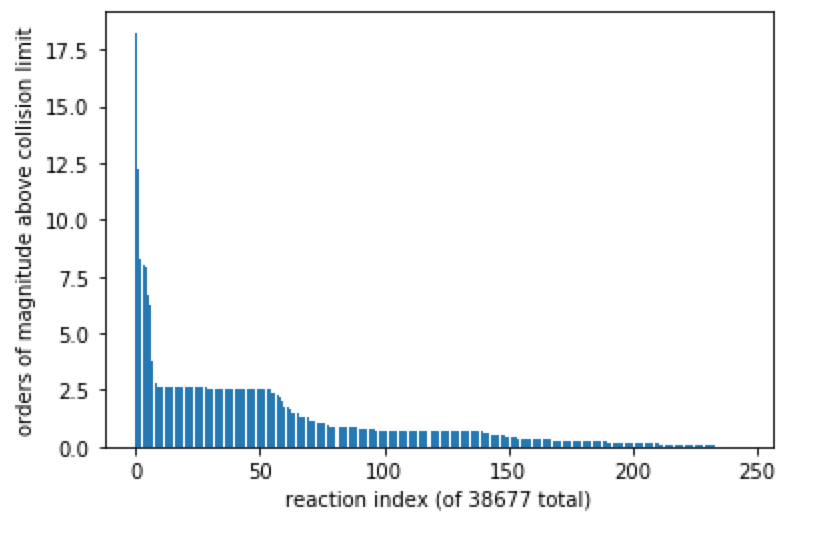
\includegraphics[scale=0.75, keepaspectratio]{images/pch-collision-violators.png}
    \caption{Collision rate violators of the initial RMG propyl-cyclohexane model based on the factor above the collision limit set by the Lennard-Jones Potential collision limit described in Wang et al. \cite{Wang2017Molecular-levelTemperature}}
    \label{fig:pch-collision-limit}
\end{figure}





The collision rate limit is defined below in equ.\ref{equ:collision limit} in RMG 
\begin{equation}
    k_{coll,i}(T)= \sqrt{\frac{8k_BT}{\pi\mu_i}}\pi d_{i}^2\Omega_{i}^{(2.2)*}
    \label{equ:collision limit}
\end{equation}
where $\mu_i$ is the reduced mass, $k_B$ is the Boltzmann constant, $d_i$ is the collision diameter and is the arithmetic average of the $\sigma$ is the Lennard-Jones parameter for the isomer and bath gas, generally taken to be 
\begin{equation}
    d_{i} \approx \frac{1}{2}(\sigma_i + \sigma_M)
\end{equation},  $\Omega^{(2.2)^*}$ is the configurational collision integral, which is parameterised as:
\begin{equation}
    \Omega_{i}^{(2.2)*} = 1.16145T^{*^{-0.14874}}+0.52487e^{-0.7732T*}+2.16178e^{-2.437887T*}
\end{equation} 
and \begin{equation}
    T^* \equiv k_BT / \sqrt{\epsilon_i\epsilon_M}
\end{equation} is the reduced temperature and $\epsilon_i$ is the Lennard-Jones $\epsilon$ parameters of the isomer and bath gas noting that $T^*$ uses the geometric average of the $\epsilon$ parameters.

The major reaction pathways of shown in fig.\ref{fig:pch-pathways} were discovered using the schematic and work of Abbasi et al.\cite{Abbasi2018KineticFormation} as well as the findings of Pousse et al. \cite{Pousse2010LeanN-Propylcyclohexane} for the major reaction classes of PCH, which used the high temperature oxidation of cyclohexane and acyclic alkanes (\ce{nC3H7}) as a basis for the discovery of reaction pathways. As a result of this discovery, the RMG PCH model applied a similar reaction pathway for the high temperature mechanism only. 

\begin{figure}[hbp]
    \centering
    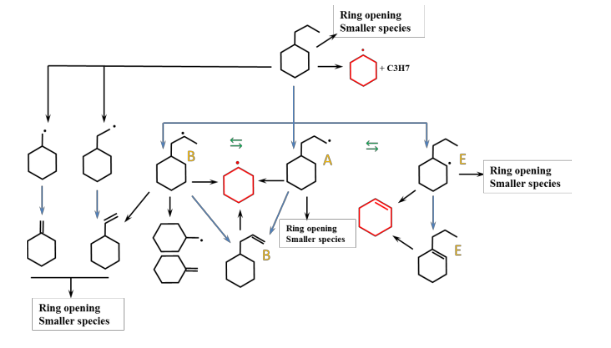
\includegraphics[scale=0.5, keepaspectratio]{images/PCH-schematic.png}
    \caption{High temperature reaction pathways of propyl-cyclohexane (PCH) as described by Abbasi et al. \cite{Abbasi2018KineticFormation}}
    \label{fig:pch-pathways}
\end{figure}


\newpage

\section{Reaction Pathways of n-propyl-cyclohexane Kinetic Model}
N-propyl-cyclohexane follows the class of reactions for its oxidation starting with a unimolecular fuel decomposition and hydrogen abstraction reactions, and further down through a series of steps. H-abstraction reactions occur at high to produce cycloalkyl radicals with different radicals sites - sites on the cyclic ring and sites on the alkyl groups. These class of reactions was proposed by Pousse et al.\cite{Pousse2010LeanN-Propylcyclohexane} in the oxidation mechanism of n-propyl-cyclohexane as a constituent of diesel fuel surrogates. 

At high temperatures, H-abstraction reactions occur via a $\beta$-scission - simply meaning that when the H-atom is removed, the radical is formed on the adjacent carbon atom to ensure thermodynamic stability. Nonetheless, since at high temperatures, there is sufficient energy and collisions occur more rapidly, the radical though stable isomerizes and forms other radicals within the cycloalkyl radical atom with molecular formula \ce{C9H17}. These radicals can also form if the ring decomposes along the \ce{C-C} bonds through $\beta$-scissions and letting go of yet another hydrogen to form a first a biradical and then a double bond - olefins (propenyl-cyclohexane or propyl-cyclohexene) with another radical species, thus having a combination of Intra\textunderscore RH\textunderscore Add\textunderscore Endocyclic reactions to produce acyclic nonene in fig.\ref{fig:nonene } and that of R\textunderscore Addition\textunderscore MultipleBond on the cycloalkyl radicals to give propenyl-cyclohexane (double bonds on the alkyl group) and propyl-cyclohexene (double bond on the ring) through $\beta$-scissions.
  
  
  \begin{figure}[!htp]
      \centering
      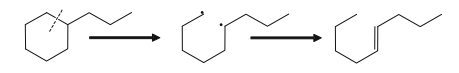
\includegraphics[keepaspectratio]{images/nonene.png}
      \caption{Unimolecular initiation of the PCH bonds forming acyclic nonene \cite{Pousse2010LeanN-Propylcyclohexane}}
      \label{fig:nonene }
  \end{figure}
  
\subsection{High Temperature mechanism of propyl-cyclohexane}
  From fig.\ref{fig:pch-pathways}, the main class of reactions that make up the dominant reaction pathways for PCH are:
  \begin{enumerate}
      \item Unimolecular fuel decomposition
      \item H-atom abstraction leading to cycloalkyl radicals
      \item $\beta$-scission decomposition along the \ce{C-C} bonds to give acyclic biradicals and eventually Olefins
      \item Dehydrogenation leading to benezene and smaller radicals 
      \item Isomerization and decomposition of radicals after the ring opening
  \end{enumerate}

The various stages of the reactions are dependent on temperature, thus at higher temperatures the chain branching is not as complex, however at lower temperature many reaction pathways are possible. Addition of \ce{O2} to the cycloalkyl radicals to form \ce{cyROO^.} also happens at high temperatures but is more dominant in the low temperature mechanism as well as the formation of hydroperoxy-cycloalkyl radicals eventually leading to cyclic ketohyroperoxide radicals. The final reaction flux pathways are shown in fig.\ref{fig:pch-pfa}.


\begin{figure}
    \centering
    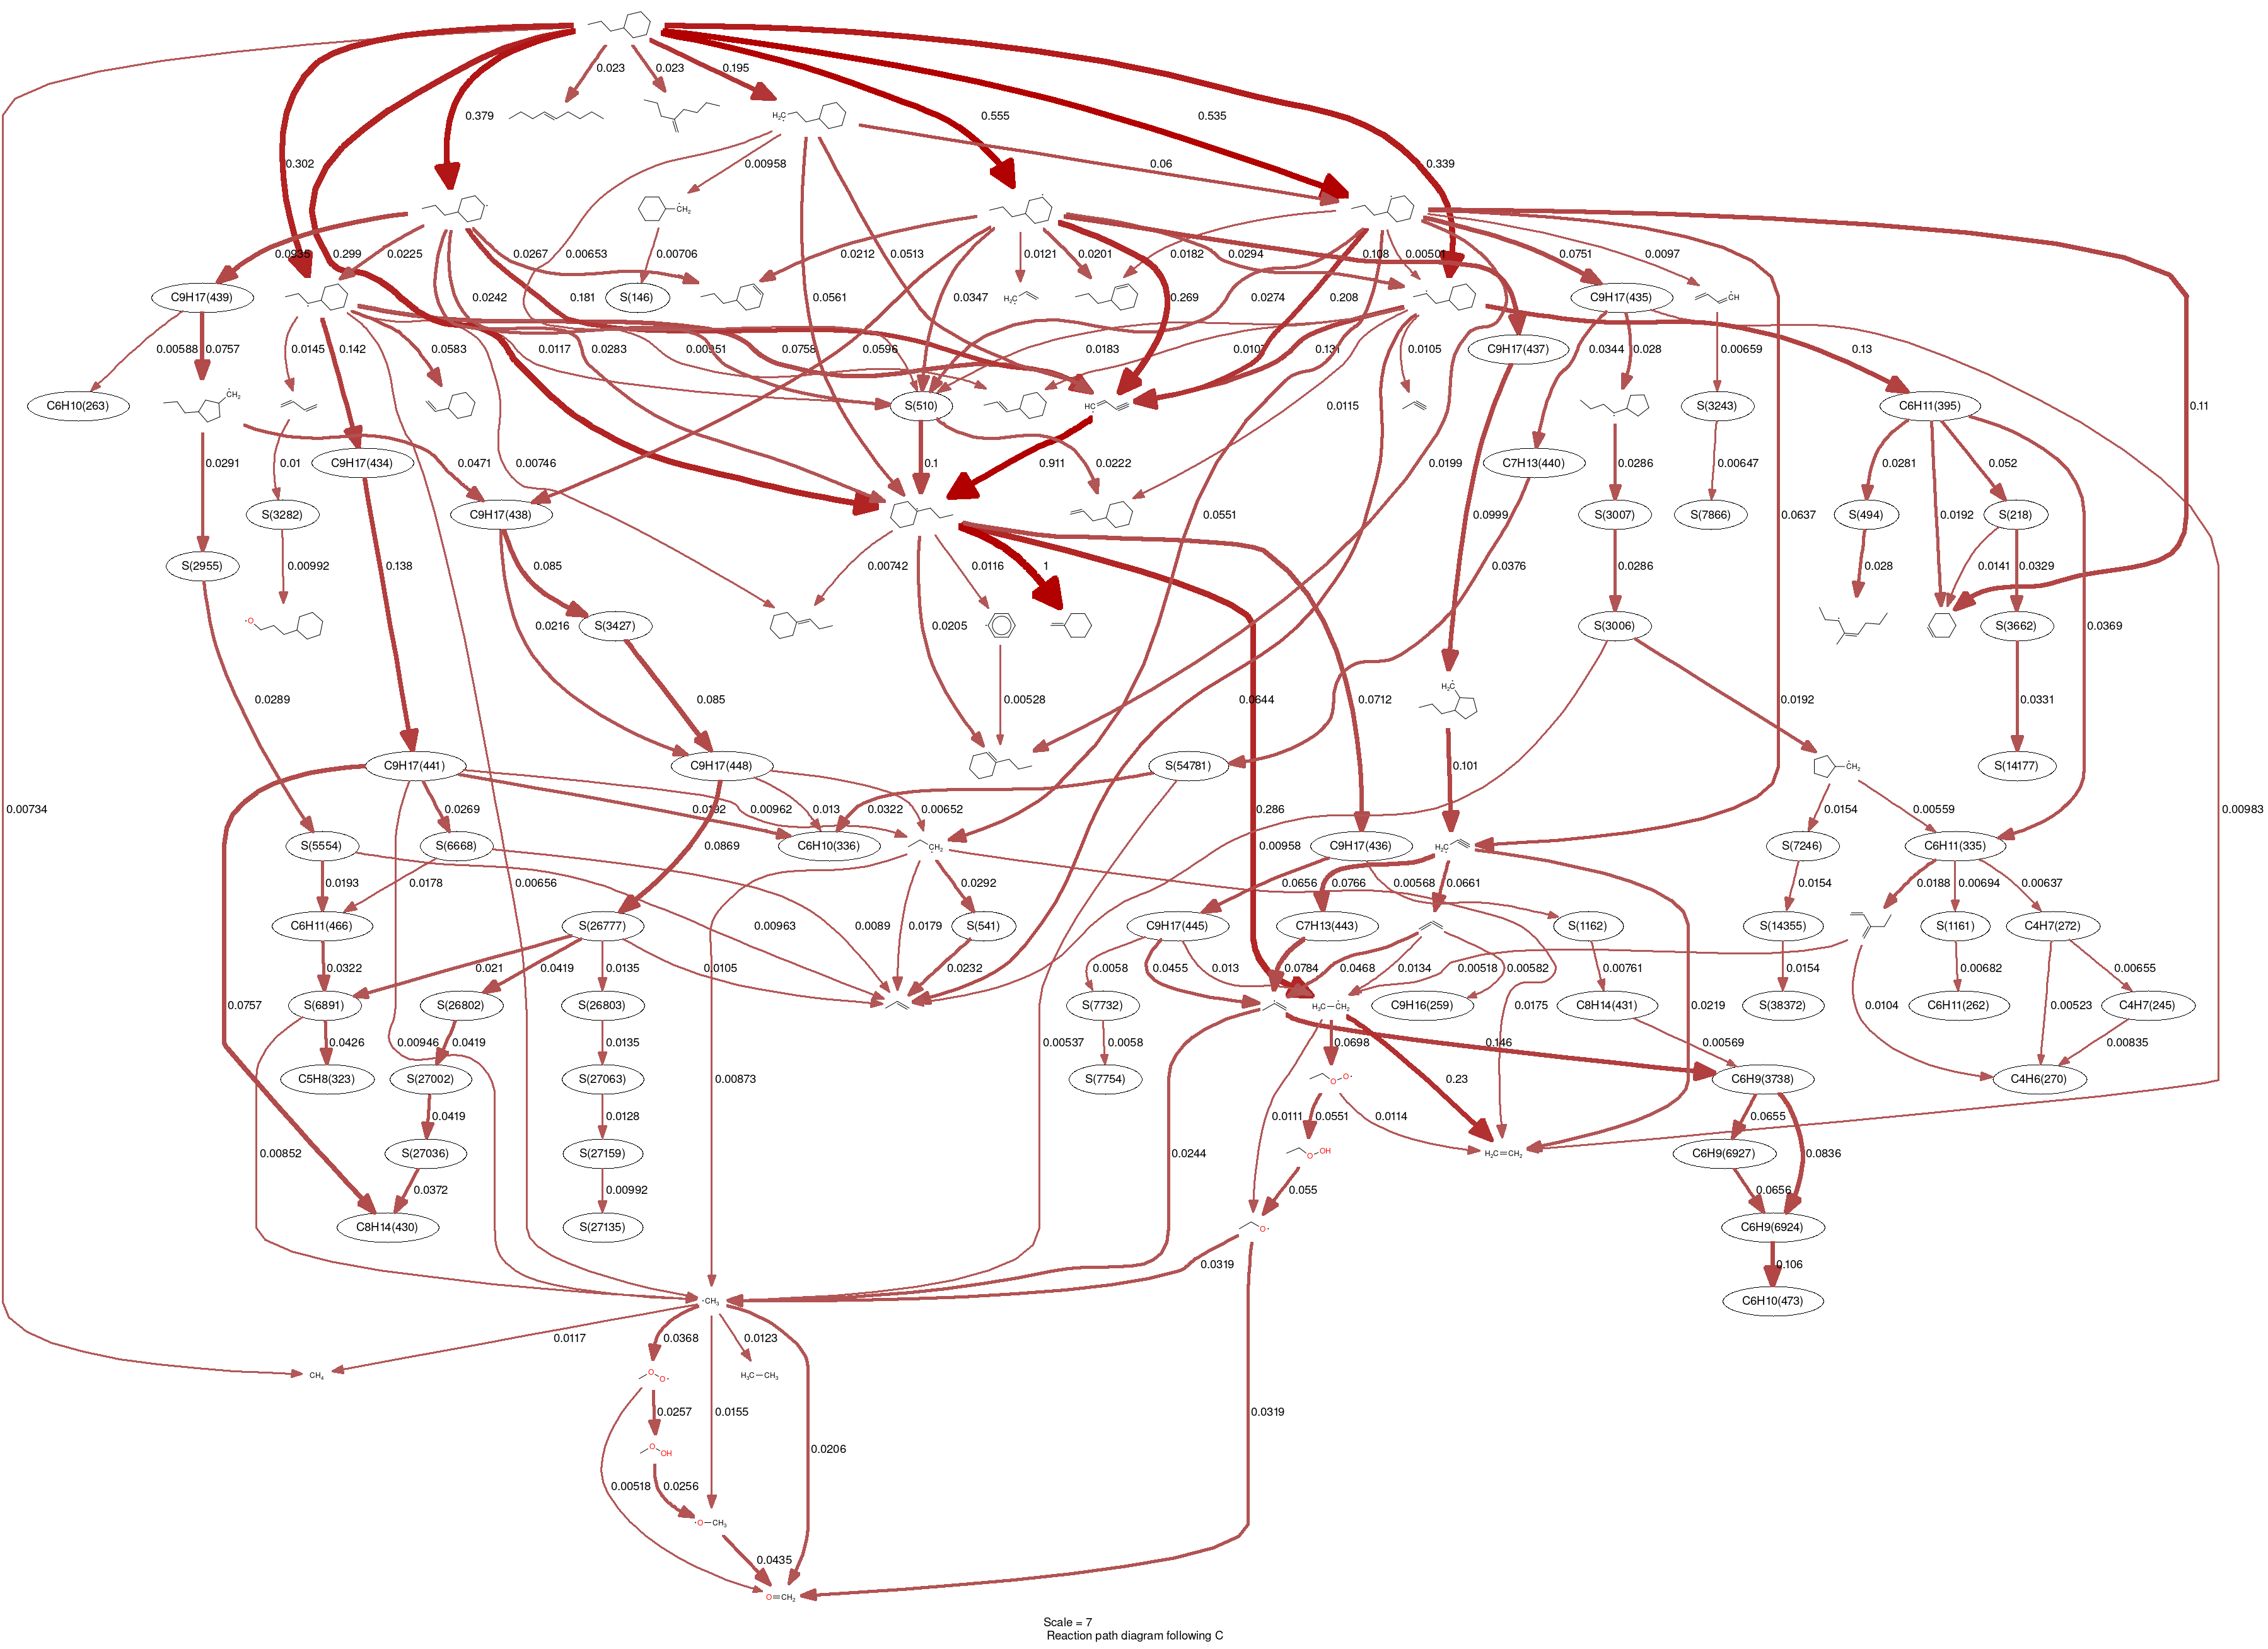
\includegraphics[scale=0.175, keepaspectratio]{images/pch-pfa.png}
    \caption{Path flux diagram of PCH model @ 1100 K and 20 atm}
    \label{fig:pch-pfa}
\end{figure}
\cleardoublepage
\subsection{Model validation of n-propyl-cyclohexane in shock tubes for ignition delay time predictions}
Shock tubes essentially devices designed to experiment and study the flow of high-temperature and high-velocity effects of compressible gases within an actual engine-like environment. It is designed on the basis of knowledge of gas dynamics and analysing shock waves. It operates on the principle that at high temperatures, supersonic gases flow is in the tube a diaphragm causes a separation into regions of high-pressure and low-pressure. As the pressure rises, an unsteady rarefied wave passes into the driver gas with a velocity usually a few kilometers per second causing flow from the high-pressure region to the low-pressure region. As the shock wave progresses in the low-pressure region, it pushes the low-pressure gas ahead of it. Thus, creating two fronts, flow ahead of the shock wave and flow behind the shock wave. The flow ahead of the behind the shock wave (driver gas) is the gas of interest. The velocity of the driver gas is equal to  that of the driven gas\cite{Greene1964TheR.}. Usually, there in the high-pressure region, is an explosive gas which is the gas studied, and present is a laser beam to detect the luminescence of some excited species. The ignition delay time can be defined as the time it takes:
\begin{enumerate}
    \item For the shock wave to hit the wall and propagate with the excitation of a \ce{CH*} or \ce{OH*}radical
    \item For the shock wave to hit the wall and measurement of the highest peak of the temperature in the driven section
    \item For the shock wave to hit the wall and detection of the highest peak of the pressure in the driven section
\end{enumerate}
Since all three possibilities of measuring the ignition delay time data in shock tubes exist, it is often well defined based on one of the three main possibilities usually for the first-stage ignition \cite{Davidson2004InterpretingData}\cite{Fieweger1994Shock-tubePressures}\cite{Fieweger1997Self-ignitionPressure}\cite{Pfahl1996Self-ignitionConditions}\cite{Haylett2012IgnitionTube}

In Cantera, this process is often defined based on the reactor type of interest. First, the gas solution object is created with the \textbf{gas.Solution} class, then a reactor type is selected with the appropriate initial conditions usually coming from the experimental data being validated against. Next, the state of the system is set with the reactor network previously defined and then a simulation in time for the next states is found using the ODE solver. The ODE solver starts at the current state  of the systems and progresses in time by one of the following methods:
\begin{enumerate}
    \item \textbf{step()}: This involves a reactor step from the current state of the system by solving the previous state of the system using the time step given. This is an explicit method where the ODE solver internally solves the numerical Differential Algebraic Equations (DAE) system. The new time is returned as well as the state of the system at the next state using the previously defined time step $\Delta$t within the solver absolute and relative tolerances. The time step cannot be larger than the maximum time step or else the ODE solver breaks.
    \item \textbf{advance($t_{new}$)}: This method solves the state of the system at a predefined step times $t_{new}$. This $t_{new}$ describes the absolute time of the system from the initial system by calling the ignition delay time function for the reactor in a loop, either a while loop or for loop at exactly the time specified - basically using the \textbf{step():} function several times in the process. In addition, the \textbf{advance():} function can be made to continue until a steady-state solution is attained by time stepping. Only when the feature-scaled residual of the state vector is below a given threshold value is the system at steady-state and the ODE solver stops.
\end{enumerate} 
For all shock tube models in this work, a zero-dimensional homogeneous closed ideal gas reactor with constant volume and internal energy class was used since at constant volume, there is no P-V work done against the control volume of the gas. Since the temperature is known, the energy equation is computed assuming adiabatic conditions in the reactor volume. The time integration of the species is computed in uniform time steps until the solution is found. During the time integration, the reactor model scheme usually an ODE SUNDIALS solver \cite{hindmarsh2005sundials} solves the differential equations of the species within the energy equation. The energy equation accounts for the energy interaction via the heat equation but is ignored since the reactor assumes adiabatic conditions and indicates only mechanical work interactions, mass transport due to species diffusion and conversion.  The equation being solved in the ideal gas reactor  of Cantera is equation \ref{eq.mass conservation} as given by Robert Kee et al's book on Chemically Reacting Flow \cite{Kee2003ChemicallyPractice}. The definition of the ignition delay time varies. Nonetheless, the model used in Cantera assumes an ignition delay time based on the excited \ce{CH} or \ce{OH} radical species and is often very close to the highest temperature spike Ji et al point out for the sensitivity analysis of ignition delay times \cite{Ji2019EvolutionAutoignition}. 

\begin{equation}
    U = m\sum_k{Y_k u_k(T)}
\end{equation}

\begin{equation}
    \frac{dU}{dt} = u\frac{dm}{dt}+mc_v\frac{dT}{dt}+m\sum_k{u_k \frac{dY_k}{dt}}
\end{equation}

\[\text{Substituting the corresponding derivations for temperature in the reactor as:} \]


\begin{equation}
    mc_v\frac{dT}{dt}=-p\frac{dV}{dt} - Q^. + \sum_{in}{m_{in}(h_{in}- \sum_k{u_k Y_{k, in}}) -\frac{pV}{m}\sum_{out}{m_{out}^.} - \sum_k{m_{k, gen}^. u_k}}
    \label{eq.mass conservation}
\end{equation}

The ignition delay times prediction are presented as modeled in Cantera against shock tube experiments of Dubois et al.\cite{Dubois2009ExperimentalConditions} and Tian et al. \cite{Tian2014ComparativeN-Propylcyclohexane} .

As seen in fig. \ref{fig:pch-idt-dubois}, there is close agreement at to experiments of Dubois et al.\cite{Dubois2009ExperimentalConditions} who studied n-prpylcyclohexane under engine-like conditions in a shock tube and spherical bomb using the chemiluminescence of \ce{OH^*} and \ce{CH^*}radicals for the ignition delay of PCH \ \ce{O2} \ \ce{Ar} mixtures for $\phi=0.2$, $\phi=0.3$, $\phi=0.4$ and $\phi=0.5$ at 10 bar. As the model progresses further, there is more deviation between the model prediction of ignition delay times against the experiments of Tian et al. who studied the ignition delay times of several cyclohexane fuels - cyclohexane, ethylcyclohexane and n-propylcyclohexane at atmospheric pressure between lean, stoichiometric and rich fuel mixtures. The prediction at $\phi=2.0$ is unpredicted and a sensitivity analysis would be helpful to understand which reactions control the ignition delay time predictions.


\begin{figure}[!hbp]
    \centering
    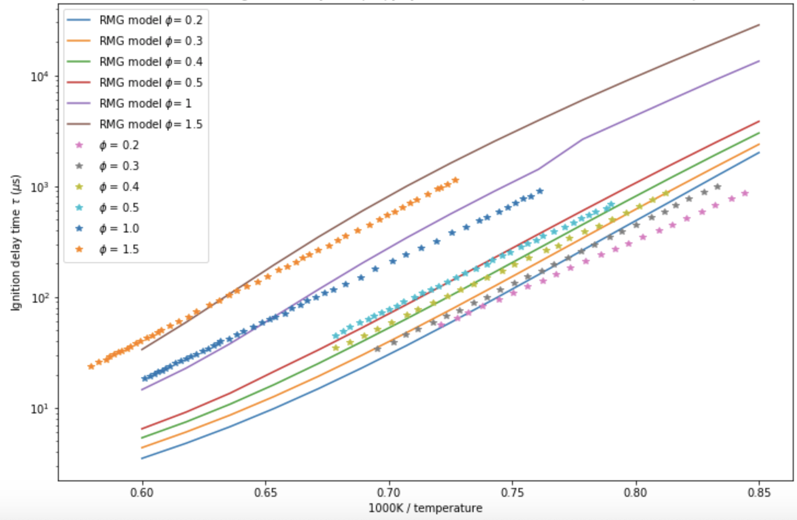
\includegraphics[scale=0.4, keepaspectratio]{images/pch-idt-dubois.png}
    \caption{Ignition delay time prediction of propyl-cyclohexane/air at 10 bar for $\phi=0.2$,$\phi=0.3$,$\phi=0.4$, $\phi=0.5$, $\phi=1.0$ and $\phi=1.5$ against experiments of Dubois et al. \cite{Dubois2009ExperimentalConditions}. Lines indicate model predictions and symbols indicate experiments}
    \label{fig:pch-idt-dubois}
\end{figure}



\begin{figure}[!htp]
    \centering
    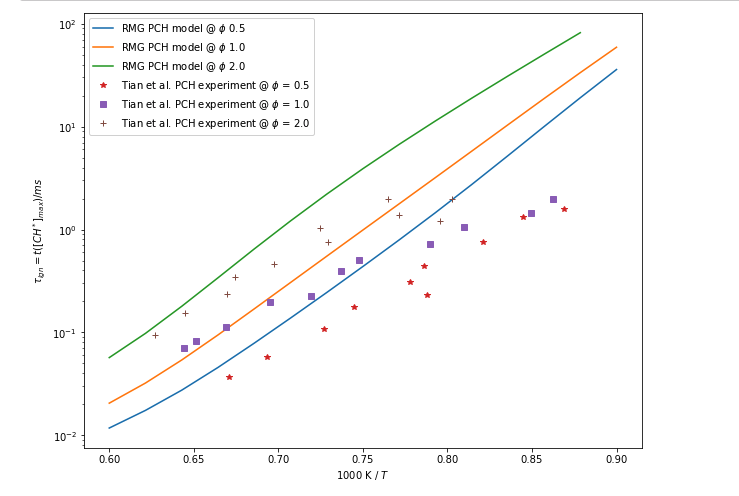
\includegraphics[scale=0.4, keepaspectratio]{images/pch-model-idt.png}
    \caption{Ignition delay time prediction of propyl-cyclohexane/air at 1 atm for $\phi=0.5$, $\phi=1.0$ and $\phi=2.0$ against experiments of Tian et al. \cite{Tian2014ComparativeN-Propylcyclohexane}. Lines indicate model predictions and symbols indicate experiments}
    \label{fig:pch-idt}
\end{figure}


\subsubsection{Sensitivity Analysis of the Ignition delay times}
A detailed analysis was done to determine which control variables control the ignition delay of the iso-octane model. Since the species usually measured for the onset of ignition is the \ce{OH^.} radical \cite{Ji2019EvolutionAutoignition}, the concentration of the \ce{OH^.} radical was used as the criteria for sensitivity by the use of a brute force method comparing the localised sensitivity at a given temperature for all the top 10 most sensitive reactions that influence the ignition delay time. This sensitivity analysis was done at high temperatures of 1250 K to observe which reactions contribute the most to either the production or consumption of the \ce{OH^.} radical species. 

The sensitivity analysis involves the perturbation of both the forward and reverse rates of the 20 most sensitive reactions to \ce{OH^.} radical concentration by a factor of two and then comparing the change in the ignition delay time to the preset (original )rate constant of those same reaction ignition delay time sensitivity coefficients to the \ce{OH^.} radical species. The magnitude of the sensitivity coefficient indicates a strong dependence on \ce{OH^.} radical concentration, while the sign indicates rate of production if positive and rate of consumption if negative. The sensitivity plots are shown in fig.\ref{fig:pch-sensitivity}.

The summary of the RMG n-propyl-cyclohexane model is given in table \ref{tab:pch_model_summary}. 
\begin{table}[ht]
\arrayrulecolor[HTML]{DB5800}
\caption{Summary of RMG n-propyl-cyclohexane model analysis and Ignition delay time prediction at extinction }
\centering
\begin{adjustbox}{width=1\textwidth}
\begin{tabular}{ p{6cm} c c c c }
\rowcolor{lightgray}\multicolumn{4}{|c|}{RMG n-propyl-cyclohexane model summary} \\
Number of Species before model generation stopped & 682 & &  \\ 
Number of species after model generation stopped  & 851 & &  \\
Number of Reactions before model generation stopped & 29174 & & \\ 
Number of reactions after model generation stopped & 49638 & & \\ 
\hline
 Model ignition delay time at extinction &  Temperature & Pressure & Equivalence ratio \\
 \begin{tabular}{ c }
    $\tau$=35.8521 ms   \\
    $\tau$=59.0368 ms \\ 
    $\tau$=81.7375 ms \\
 \end{tabular} & \begin{tabular}{ c } 
       1111.11 K\\
      1111.11 K \\
      1111.11 K \\
 \end{tabular} & 1 atm & \begin{tabular}{ c }
      $\phi=0.5$  \\
      $\phi=1.0$ \\
      $\phi=2.0$ \\
 \end{tabular} \\
 \end{tabular}
    \end{adjustbox}
    \label{tab:pch_model_summary}
\end{table}


\begin{figure}
    \centering
    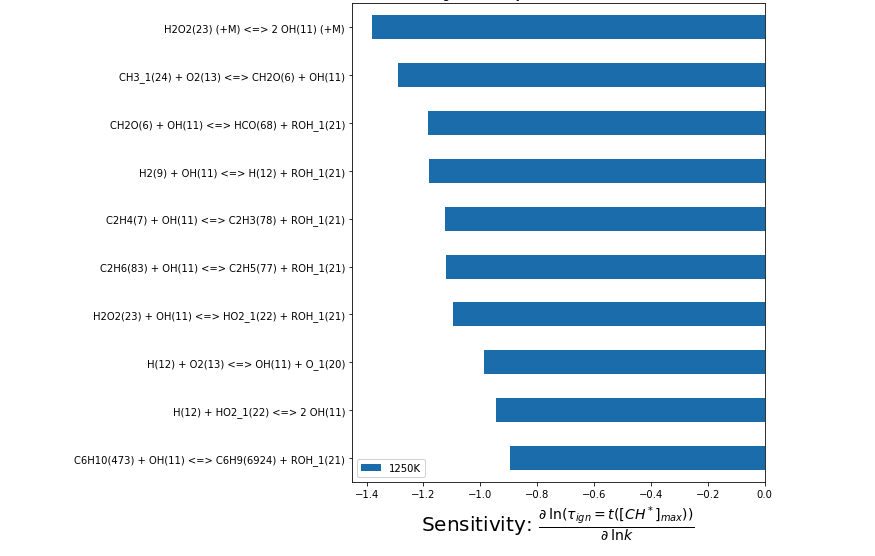
\includegraphics[scale=0.45, keepaspectratio]{images/pch-sensitivity.png}
    \caption{Sensitivity coefficients of the ignition delay time of the n-propyl-cyclohexane model to \ce{OH^.} radical concentration at stoichiometric fuel/air mixture at 1250 K at $P=1$ atm. Where the ignition delay times $\tau_{ign}=t(\ce{CH^.}_{max})$}
    \label{fig:pch-sensitivity}
\end{figure}


\chapter{Blended GTL fuel models}

\section{GTL fuel composition}


Synthetic jet fuels have become an area of increasing interest, in order to curb the emissions and pollution levels in air transportation dependent on conventional oil-derived jet fuels \cite{RePEc:eee:energy:v:43:y:2012:i:1:p:111-123}. As a result of this interest as well as mission to reduce the over-dependence on conventional oil-derived fossil fuels and reduce carbon footprint, future designs of aero-propulsion engines will rely on the computational modeling of sustainable and alternative jet fuels \cite{Corporan2007EmissionsFuel}\cite{Hermann2006ChemicalFuel}. Chapter 1 and 2 has gone in detail on the need for the computational modeling of jet fuel as well as jet fuel fuel surrogates. Since, predictions of jet fuel combustion kinetics is central to the fuel reactivity in aero-propulsion engines, parameters such as auto-ignition properties of the fuel surrogates is necessary to understand its behavior under engine-like conditions. 

The most common parameter used is the ignition delay time and it is heavily dependent on the combustion kinetics as well as the macroscopic characteristics of temperature, pressure and mixture composition fractions of the fuel. Jet fuels typically contain thousands of both major and minor constituents and as such modeling a real jet fuel is not viable due to the complexity as well as computational resources required. The use of surrogate models are applicable based on the major constituents of the jet fuel, where the physical properties are carefully chosen to match the physical characteristics of the fuel and that of the chemical properties tested and modeled under carefully chosen conditions \cite{Edwards2001SurrogateFuels}\cite{Huber2008SurrogateCurve}. While all of this major aspects of surrogate models have been covered in chapter 2, more emphasis is laid in this chapter on the constituents of various alternative jet fuels and specifically on F-T GTL fuel blend mixtures.


\vspace{2cm}


Experimental investigation of alternative jet fuel includes ignition delay time measurements in shock tubes and rapid compression machines (RCM) \cite{Dean2007AutoignitionPressures}\cite{Wang2012}\cite{Malewicki2013ExperimentalN-dodecane}\cite{Dagaut2014}\cite{Dagaut2014CombustionModeling}\cite{Dagaut2016ExperimentalSurrogates}\cite{Askari2016}\cite{Valco2016LowMachine}, laminar flame speeds \cite{Singh2011ExperimentalFlames}\cite{Wang2012}\cite{Hui2013LaminarPressures}\cite{Dagaut2014}\cite{Yu2016TheoreticalFuel}, chemical structure from pyrolysis and oxidation in pressure flow reactors as well as oxidation in a jet stirred \cite{Gokulakrishnan2007ExperimentalConditions}\cite{Gokulakrishnan2008IgnitionFuel}\cite{Honnet2009AKerosene}\cite{Dooley2010AProperties}\cite{Mze-Ahmed2010KineticsStudy}\cite{Dagaut2014CombustionModeling}\cite{Dagaut2014}\cite{Dagaut2015TheStudy}\cite{Dagaut2016ExperimentalSurrogates}, emissions in a gas turbine combustor rig \cite{Hermann2006ChemicalFuel}. These experimental measurements provide a basis with which to compare chemical kinetic models of jet fuel surrogates as a means of validating the mechanisms. 

Similarly, several kinetic models of jet fuel surrogates have been published over the years using the chemical kinetic mechanism generation code PSR \cite{Glarborg1986PSR:Reactors} a Fortan solver for simulating well-stirred reactors used by Mzé-Ahmed and others in the mechanism of a synthetic jet fuel \cite{Mze-Ahmed2010KineticsStudy}, models have also been published on F-T synthetic surrogate fuels using the CHEMKIN suite code from Naik et al \cite{Naik2011DetailedFuels}, F-T GTL surrogate models have also been deduced based on surrogate modeling of jet aviation fuels using a three-component fuel surrogate model of n-decane, iso-octane and toluene as described by Dooley et al \cite{Dooley2010MethylModel}. Ranzi et al. followed up with a more compact model of jet fuel model up to \ce{C_16} \cite{Ranzi2012HierarchicalFuels} with more than 8000 reactions and more than 250 species. Although, skeletal models of GTL models have been built in the past by Dagaut et al \cite{Dagaut2014}, more recently, Dagaut et al \cite{Dagaut2016ExperimentalSurrogates} built a detailed model of a GTL mechanism with 3 components with more than 10000 reversible reactions and more than 2000 species. The reaction pathways of these models are representive of the individual PRFs used in the mechanism generation.


The GTL fuel composition was based on the composition as defined by Dagaut et al in the work on the experimental and modeling of GTL fuel surrogates \cite{Dagaut2014}. The summary of the GTL fuel surrogate used in this work and the comparison to the real fuel is in table \ref{tab:GTL_model_summary}.


\begin{table}[ht]
\arrayrulecolor[HTML]{DB5800}
\caption{Summary of RMG GTL fuel surrogate model composition}
\centering
\begin{adjustbox}{width=1\textwidth}
\begin{tabular}{ p{6cm} c c c c c }
\rowcolor{lightgray}\multicolumn{5}{|c|}{RMG iso-octane model summary} \\
 Fuel &  Fuel composition &  (\% weight) & Fuel properties & Experimental conditions \\
 GTL & \begin{tabular}{ c }
    n-Paraffins:  \\ 
    iso-Paraffins \\
    di-Naphthenes \\
    mono-Naphthenes \\ 
    Aromatics \\
 \end{tabular} & \begin{tabular}{ c } 
       28.1 \\
      62.8  \\
     8.2 \\
     0.6 \\
     0.2 \\
 \end{tabular} & \begin{tabular}{ c }
      \ce{C_{10.45}H_{23.06}}  \\
       Hydrogen-Carbon ratio (H/C) : 2.20 \\
      Cetane Number (CN): $58.0^a$ \\
       Density $\rho$: 737 g/L \\
 \end{tabular} & \begin{tabular}{ c }
      $\phi = 1.0$  \\
      Temperature range: 560 - 1110 K \\
      10,450 ppm of C \\
 \end{tabular} \\ 
 \hline 
 GTL Surrogate & \begin{tabular}{ c }
      n-decane  \\
      iso-octane \\
      n-propyl-cyclohexane \\
 \end{tabular} & \begin{tabular}{ c }
      57.7  \\
      33.2 \\
      9.1 \\
 \end{tabular} & \begin{tabular}{ c }
      $\ce{C_{10.45}H_{22.95}}^a$ \\
      Hydrogen-Carbon ratio (H/C) : 2.1966 \\
      Derived Cetane Number (CN): 54.5 \\
       Density ($\rho$) at $15^{\circ}C$: 723 g/L \\
       Molar weight $148.31^a$ g/mol \\
       \hline
       $^a 1.13\times \ce{C_{9.2451}H_{20.308}}$ since 1130 ppm of model fuel was used to present 1000 ppm of GTL
 \end{tabular} & \begin{tabular}{ c }
      $\phi = 1.0$  \\
      Temperature range: 560 - 1110 K \\
      10,450 ppm of C \\
 \end{tabular} \\
 \end{tabular}
    \end{adjustbox}
    \label{tab:GTL_model_summary}
\end{table}

Kinetic models of jet fuels in previous studies in summarized in table \ref{tab:GTL_model_summary} while the path flux diagram of the GTL model fuel blend is show in fig.\ref{fig:gtl-pfa}





\subsection{Model validation of F-T GTL surrogate fuel model in shock tubes for ignition delay time predictions}

Shock tubes essentially devices designed to experiment and study the flow of high-temperature and high-velocity effects of compressible gases within an actual engine-like environment. It is designed on the basis of knowledge of gas dynamics and analysing shock waves. It operates on the principle that at high temperatures, supersonic gases flow is in the tube a diaphragm causes a separation into regions of high-pressure and low-pressure. As the pressure rises, an unsteady rarefied wave passes into the driver gas with a velocity usually a few kilometers per second causing flow from the high-pressure region to the low-pressure region. As the shock wave progresses in the low-pressure region, it pushes the low-pressure gas ahead of it. Thus, creating two fronts, flow ahead of the shock wave and flow behind the shock wave. The flow ahead of the behind the shock wave (driver gas) is the gas of interest. The velocity of the driver gas is equal to  that of the driven gas\cite{Greene1964TheR.}. Usually, there in the high-pressure region, is an explosive gas which is the gas studied, and present is a laser beam to detect the luminescence of some excited species. The ignition delay time can be defined as the time it takes:
\begin{enumerate}
    \item For the shock wave to hit the wall and propagate with the excitation of a \ce{CH*} or \ce{OH*}radical
    \item For the shock wave to hit the wall and measurement of the highest peak of the temperature in the driven section
    \item For the shock wave to hit the wall and detection of the highest peak of the pressure in the driven section
\end{enumerate}
Since all three possibilities of measuring the ignition delay time data in shock tubes exist, it is often well defined based on one of the three main possibilities usually for the first-stage ignition \cite{Davidson2004InterpretingData}\cite{Fieweger1994Shock-tubePressures}\cite{Fieweger1997Self-ignitionPressure}\cite{Pfahl1996Self-ignitionConditions}\cite{Haylett2012IgnitionTube}

In Cantera, this process is often defined based on the reactor type of interest. First, the gas solution object is created with the \textbf{gas.Solution} class, then a reactor type is selected with the appropriate initial conditions usually coming from the experimental data being validated against. Next, the state of the system is set with the reactor network previously defined and then a simulation in time for the next states is found using the ODE solver. The ODE solver starts at the current state  of the systems and progresses in time by one of the following methods:
\begin{enumerate}
    \item \textbf{step()}: This involves a reactor step from the current state of the system by solving the previous state of the system using the time step given. This is an explicit method where the ODE solver internally solves the numerical Differential Algebraic Equations (DAE) system. The new time is returned as well as the state of the system at the next state using the previously defined time step $\Delta$t within the solver absolute and relative tolerances. The time step cannot be larger than the maximum time step or else the ODE solver breaks.
    \item \textbf{advance($t_{new}$)}: This method solves the state of the system at a predefined step times $t_{new}$. This $t_{new}$ describes the absolute time of the system from the initial system by calling the ignition delay time function for the reactor in a loop, either a while loop or for loop at exactly the time specified - basically using the \textbf{step():} function several times in the process. In addition, the \textbf{advance():} function can be made to continue until a steady-state solution is attained by time stepping. Only when the feature-scaled residual of the state vector is below a given threshold value is the system at steady-state and the ODE solver stops.
\end{enumerate} 
For all shock tube models in this work, a zero-dimensional homogeneous closed ideal gas reactor with constant volume and internal energy class was used since at constant volume, there is no P-V work done against the control volume of the gas. Since the temperature is known, the energy equation is computed assuming adiabatic conditions in the reactor volume. The time integration of the species is computed in uniform time steps until the solution is found. During the time integration, the reactor model scheme usually an ODE SUNDIALS solver \cite{hindmarsh2005sundials} solves the differential equations of the species within the energy equation. The energy equation accounts for the energy interaction via the heat equation but is ignored since the reactor assumes adiabatic conditions and indicates only mechanical work interactions, mass transport due to species diffusion and conversion.  The equation being solved in the ideal gas reactor  of Cantera is equation \ref{eq.mass conservation} as given by Robert Kee et al's book on Chemically Reacting Flow \cite{Kee2003ChemicallyPractice}. The definition of the ignition delay time varies. Nonetheless, the model used in Cantera assumes an ignition delay time based on the excited \ce{CH} or \ce{OH} radical species and is often very close to the highest temperature spike Ji et al point out for the sensitivity analysis of ignition delay times \cite{Ji2019EvolutionAutoignition}. 

\begin{equation}
    U = m\sum_k{Y_k u_k(T)}
\end{equation}

\begin{equation}
    \frac{dU}{dt} = u\frac{dm}{dt}+mc_v\frac{dT}{dt}+m\sum_k{u_k \frac{dY_k}{dt}}
\end{equation}

\[\text{Substituting the corresponding derivations for temperature in the reactor as:} \]


\begin{equation}
    mc_v\frac{dT}{dt}=-p\frac{dV}{dt} - Q^. + \sum_{in}{m_{in}(h_{in}- \sum_k{u_k Y_{k, in}}) -\frac{pV}{m}\sum_{out}{m_{out}^.} - \sum_k{m_{k, gen}^. u_k}}
    \label{eq.mass conservation}
\end{equation}

The ignition delay times prediction are presented as modeled in Cantera against shock tube experiments of Wang et al.\cite{Wang2012}.

\begin{table}[ht]
\arrayrulecolor[HTML]{DB5800}
\caption{Summary of kinetic mechanisms of jet fuel surrogates composition}
\centering
\begin{adjustbox}{width=1\textwidth}
\begin{tabular}{ p{6cm} c c c c c }
\rowcolor{lightgray}\multicolumn{5}{|c|}{RMG iso-octane model summary} \\
 Fuel &  Surrogate fuel model composition &  (\% composition) & kinetic model species and reactions & Reference \\
 \hline
 GTL synthetic paraffinic kerosene (SPK) & \begin{tabular}{ c }
      n-decane  \\
      iso-octane \\
      n-propyl-cyclohexane \\
 \end{tabular} & \begin{tabular}{ c }
      57.7  \\
      33.2 \\
      9.1 \\
 \end{tabular} & Low temperature and high temperature mechanism; 1876 species and 23127 reactions & Current Study \\
 \hline
 Jet A & \begin{tabular}{ c }
    n-decane \\
    iso-octane \\
    toluene \\
 \end{tabular} & \begin{tabular}{ c } 
       42.67 \\
      33.02  \\
      24.31 \\
 \end{tabular} & Low temperature and high temperature mechanism; 753 species and 9980 reactions without PAH mechanism & Dooley et al. \cite{Dooley2010AProperties} \\
 \hline 
 S-8 & \begin{tabular}{ c }
      n-decane  \\
      iso-octane \\
      n-dodecane \\
 \end{tabular} & \begin{tabular}{ c }
      25.0  \\
      32.0 \\
      43.0 \\
 \end{tabular} & High temperature mechanism; 597 species and 4668 reactions & Naik et al. \cite{Naik2011DetailedFuels}\\
 \hline
 Shell GTL & \begin{tabular}{ c }
      n-decane  \\
      iso-octane \\
      n-dodecane \\
 \end{tabular} & \begin{tabular}{ c }
      61.0  \\
      28.0 \\
      11.0 \\
 \end{tabular} & High temperature mechanism; 597 species and 3854 reactions & Naik et al. \cite{Naik2011DetailedFuels}\\
 \hline
 GTL synthetic paraffinic kerosene (SPK) & \begin{tabular}{ c }
      n-decane  \\
      iso-octane \\
      n-propyl-cyclohexane \\
 \end{tabular} & \begin{tabular}{ c }
      65.2  \\
      37.5 \\
      10.3 \\
 \end{tabular} & Low temperature and high temperature mechanism; 2182 species and 8347 reactions & Dagaut et al. \cite{Dagaut2014} \\
 \end{tabular}
    \end{adjustbox}
    \label{tab:GTL_model_summary}
\end{table}



As seen in fig. \ref{fig:gtl-blend-idt}, there is close agreement at to experiments of Wang et al.\cite{Wang2012} who studied three jet fuels, conventional jet fuels Jet A and JP 8, two F-T GtL fuels, S-8 and Shell GtL and one F-T coal-to-liquid Sasol IPK under engine-like conditions in a shock tube using the chemiluminescence of \ce{OH^*} radicals for the ignition delay time measurement of the jet fuel mixtures with air for $\phi=1.0$ at 20 atm. The NTC regime of the RMG model of the GTL fuel surrogate is not as pronounced and a sensitivity analysis would aid knowing which reactions are most sensitive to the onset of ignition in the low temperature mechanism region.


\begin{figure}[hbp]
    \centering
    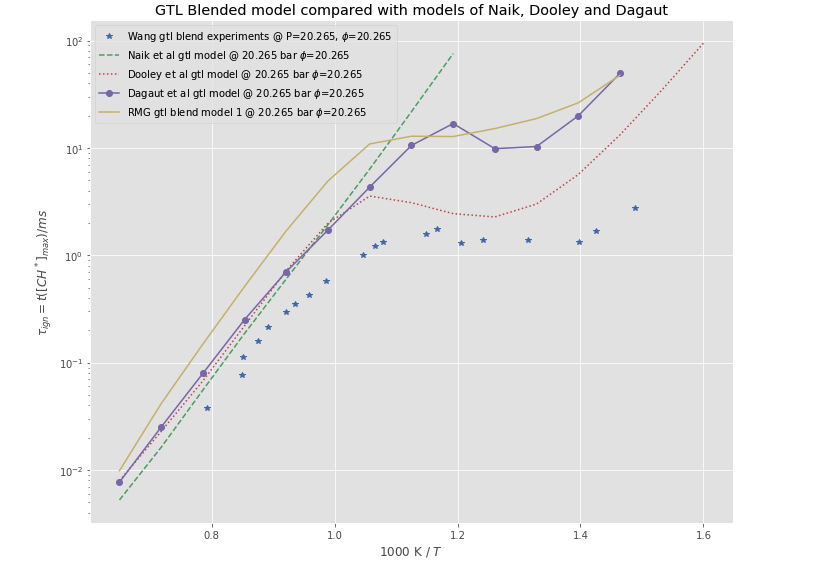
\includegraphics[scale=0.5, keepaspectratio]{images/GTL_model_blend_idt.png}
    \caption{Ignition delay times of GTL cross-reacted fuel blend with models of Naik et al. \cite{Naik2011DetailedFuels}, Dooley et al. \cite{Dooley2010AProperties}, Dagaut et al. \cite{Dagaut2014} compared against shock tube experiments of Wang et al. \cite{Wang2012} at 20 atm and stoichiometric conditions with air. Lines represent model predictions and symbols experimental measurements}
    \label{fig:gtl-blend-idt}
\end{figure}
\chapter{Conclusion and Future Work}


This chapter is a summary of this thesis work. What was proposed, done and what further work is needed to capture the effect of understanding the use of surrogate models in the analysis of Fischer-Tropsch (F-T) gas-to-liquid (GTL) fuel blends.

This work centered on the use of synthetic alternatives to the conventional-oil derived fuels in heavy duty and gas turbine applications, especially aeroderivative-gas turbine fuels - jet fuels. As regards this sustainable and alternative derivatives for jet fuels, the Fischer-Tropsch (F-T) synthesis process was seen to be a viable and interesting option especially since it has been in vogue since 1925. Since the original use of converting gas to liquid fuels was done for diesel engines, research from the literature has shown its viability in jet fuels \cite{Hermann2006ChemicalFuel} as well as  HCCI engines \cite{Mati2007TheModeling}. As a result, interest in the technology for processing and synthesising F-T GTL fuels has grown over the years, especially with the advent of renewable energy technologies in a quest to reduce carbon footprint and emissions level. 

The major analyses of F-T GTL blends has come from the spectrometry/chromatography analysis to determine the major constituents of these F-T GTL fuel blends. As such, major compounds include the presence of n-alkanes (n-paraffins), iso-alkanes (iso-paraffins), cyclo-alkanes (naphthenes) and sometimes aromatics. However, since aromatics have been wildly known to be responsible for the onset of soot and particulate matter (PM) in engines \cite{RoleOSTI.GOV}, these aromatics have been jettisoned for cyclo-alkanes (napthenes) with the knowledge that oxidation of naphthenes at low temperatures do produce aromatic compounds \cite{Abbasi2018KineticFormation}.

The use of chemical kinetic mechanisms to represent the behavior of these F-T GTL fuel blends has grown increasingly over the last years and since more work in being done to accelerate the growth of software technologies to match up with the demand of numerical and computational analysis of elementary reactions, especially in the reactivity and flammability of aero-propulsion engines, the role of computational combustion continues to increase. Engine designers will continue to rely heavily on the chemical kinetic mechanisms of different jet fuels to aid in CFD analyses of aero-engines. The use of direct numerical simulations (DNS) always proves very difficult and computationally expensive, thus it has become increasingly common to use a representation of a few chemical kinetic species to represent the kinetics of the overall fuel. This approach of representing complex chemical reaction kinetic networks with a simplified form is adopted in surrogate modeling in many diverse engineering applications. The use of these surrogate models is heavily relied on in chemical kinetic mechanisms of different fuels and F-T GTL fuel blends are no different in this regard. 

This thesis has employed a surrogate model for the representation of a F-T GTL fuel blend using a three component fuel of n-decane, iso-octane and n-propyl-cyclohexane in different compositions as seen in table \ref{fig:GTL-composition}. The use of these Primary Reference Fuels (PRFs) was been delved into in chapters 3, 4 and 5 including the high temperature and low temperature oxidation pathways for n-decane and iso-octane as well as the high temperature pathways of n-propyl-cyclohexane. The thermo-kinetic parameters used in estimating the model builds of each PRF was done in the Reaction Mechanism Generator (RMG) \cite{Gao2016ReactionMechanisms} using a base mechanism of previously published models seen in table \ref{tab:PRF_table1}. The seed mechanisms which serve as a base mechanism for the detailed kinetics of each of the PRF models helped in predicting the oxidation pathways as well as the rate parameters used in evaluating the detailed mechanisms. 

This thesis was proposed on the best applicable framework in which F-T GTL fuel blends can be effectively constructed using a three-component blends of n-decane, iso-octane and n-propyl-cyclohexane. The effective frameworks each have their respective drawbacks. 


\section{Concatentation of PRFs }
The first framework of concatenation of the three PRFs resulted in first building individual detailed kinetic mechanisms for n-decane, iso-octane and n-propyl-cyclohexane and using the appropriate modeling strategies (code) to validate the individual mechanisms against published experimental data that quantifies the auto-ignition characteristics of the PRFs. The PRFs were all validated against shock-tube experiments that measured the ignition delay times in zero-dimensional homogeneous reactors while the model of n-decane has an additional validation experiment with the laminar premixed flame speeds. The PRFs have been observed to be in close agreement and within reasonable uncertainties with the experimental data. While there were deviations in both the high temperature and low temperature mechanisms, the pronounced and well visible negative temperature coefficient (NTC) behavior was seen in the experimental model validation of n-decane and iso-octane. This NTC behavior was been attributed to the onset and rapid production and consumption of the oxygenated radicals in the \ce{OH^.} radicals, \ce{Q^.OOH} radicals, the cyclic ethers \ce{Q-O-R}, peroxyradicals \ce{ROO^.}, hydroperoxy radicals \ce{Q^.OOH}, hydroperoxy-alkyl-peroxy radicals \ce{HOOQOO^.}, di-hydroperoxy-alkyl radicals \ce{HOOQ^.OOH} and finally keto-hydroperoxy radicals. Since these pathways contain lots of oxygen atoms, the flux diagrams show that these pathways are competing pathways but are ultimately more favorable at low temperatures due to the low activation energies. The PRFs being concatenated based on composition implies that the greatest composition of the PRFs, ultimately determines the behavior of the model blend in the low temperature region and any onset of the NTC regime. While this concatenation method is preferred as the detailed PRFs have been well validated and rate parameters well inspected through sensitivity analyses, the parallel computing costs can be immense especially since all three-component PRFs must run in parallel while the concatenation occurs at the end removing or marking reactions as duplicate or using the order of the concatenation of the PRFs for the kinetic estimates used. This often is the go to choice especially since dealing with reactions in smaller more detailed forms removes the need for allowing model generation for long running times adequate for cross reactions to occur in the mixed form of using PRF species from the onset.




\section{Use of PRF species from the onset for cross reactions}

The second framework is the use of allowing the elementary and individual species of each PRF to be lumped together from the onset for cross reactions to occur. While this framework is the most time consuming and computationally expensive in the sense that all species must be allowed to react with themselves for a given time interval, the time it take for all reaction networks and pathways to occur can sometimes be infinite if tolerance thresholds are imposed for very accurate model generation. Thus, this brings with it the added complexity of addressing the reaction pathways as well as the rate parameter estimates based on the reaction and reaction family. While this method is used usually allows for more complete reactions, the framework alone usually results in weeks or even months of continuous model generation. 

This approach has been used in chapter 6, where the cross reactions are allowed and the F-T GTL blended model is compared with the mechanisms of Dooley et al \cite{Dooley2010AProperties}, Naik et al. \cite{Naik2011DetailedFuels}, Dagaut et al. \cite{Dagaut2014} and the experiments of ignition delay times in shock tubes of Wang et al. \cite{Wang2012}. As seen in fig.\ref{fig:gtl-blend-idt}, it is evident that the model with cross-reactions does hold up well against the models of Dooley et al \cite{Dooley2010AProperties}, Naik et al. \cite{Naik2011DetailedFuels}, Dagaut et al. \cite{Dagaut2014}. The important question that remains unanswered is the calculation on the computational cost as well as the reaction flux diagram of this method. Is it worth the minimum three weeks of high-performance computing with thermo-kinetic estimates that are highly uncertain ? The numerous questions of this method abounds and must be looked at in detail in subsequent works.

\section{Future Work and Recommendations}

The question as regards which framework represents the best approach to build a F-T GTL fuel surrogate blend that is closely matched by the experimental conditions is one that has been answered. As can be noted that obtaining the models of the PRFs namely, n-decane, iso-octane and n-propyl-cyclohexane is the prefered method sine the validation of each PRF has been guaranteed to conform well to experimental conditions. The context for further work remains. The most important further work needed is the estimation of the thermo-kinetic parameters used in modeling the GTL fuel surrogates as well as which model blend approach closely matches experimental conditions. The best approach is the concatenation of all PRFs since the detailed chemical kinetic mechanisms closely resembles the experimental data. More work is needed first in the following ways:
\begin{enumerate}
\begin{enumerate}
    \item Estimation of thermo-kinetic parameters used in the model generation of the chemical kinetic mechanisms of the PRFs as well as the cross reacted blends.
    \item The uncertainty analysis of the thermo-kinetic parameters used and how close they are to the physical occurrence of the estimates. This is so collision violators (rates that are above the collision rates are not used)
    \item Computational and numerical efficiency of the code to reduce computational cost through parallel computing
    \item Model validation against laminar premixed flame speeds by model reduction techniques such as Sensitivity Analysis \cite{Rabitz1983SensitivityKinetics},\cite{Turanyi1990SensitivityApplications}, Directed Related Graph Method (DRG) \cite{Lu2005AReduction}, Directed Related Graph with Error Propagation (DRGEP)\cite{Pepiot-Desjardins2008AnMechanisms}, Directed Related Graph with Sensitivity-Analysis (DRGASA)\cite{Sankaran2007StructureFlame}\cite{Zheng2007Experimental13-butadiene}, Directed Related Graph with Error Propagation and Sensitivity Analysis (DRGEPSA) \cite{Niemeyer2010SkeletalAnalysis}, Computational Singular Perturbation \cite{Massias1999AnData}, Rate-Controlled-Reduced-Equilibrium methods (RCCE) \cite{Keck1971Rate-controlledMixtures}, which is done to reduce these kinetic mechanisms to only the core skeletal models of only a few hundred species with unimportant reactions and species removed for easy numerical computation of reactors and engines in CFD analysis that engine designers use.
\end{enumerate}
\end{enumerate}


\addcontentsline{toc}{section}{REFERENCES}
\printbibliography[title=REFERENCES]
% \appendix
\chapter*{\centering APPENDIX}
\thispagestyle{plain}
\justifying

\begin{figure}
    \centering
    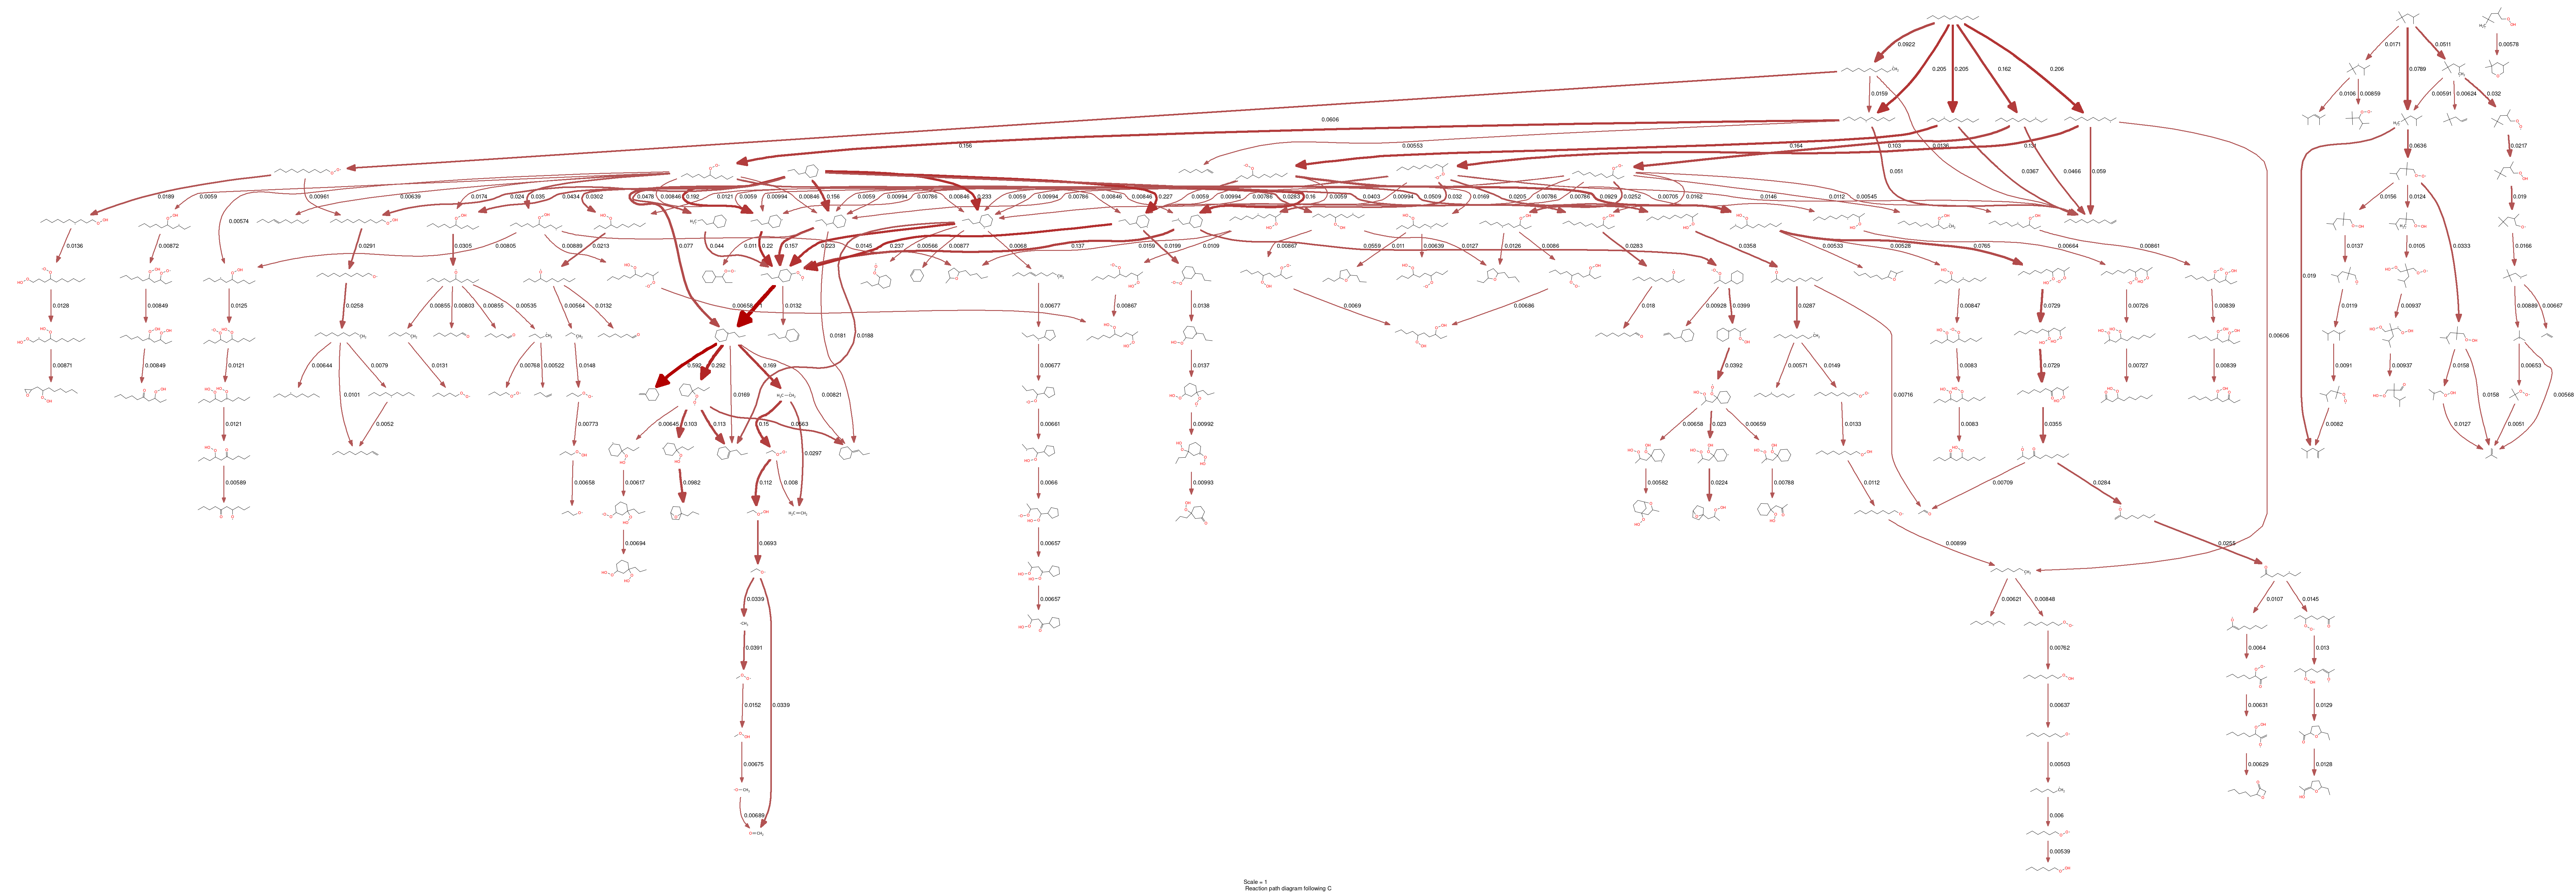
\includegraphics[scale=0.1, angle = 90, keepaspectratio]{images/GTL-PFA.png}
    \caption{Flux diagram of cross-reacted GTL fuel blend @ 900 K and 20 atm}
    \label{fig:gtl-pfa}
\end{figure}


\begin{figure}[ht]
     \centering
     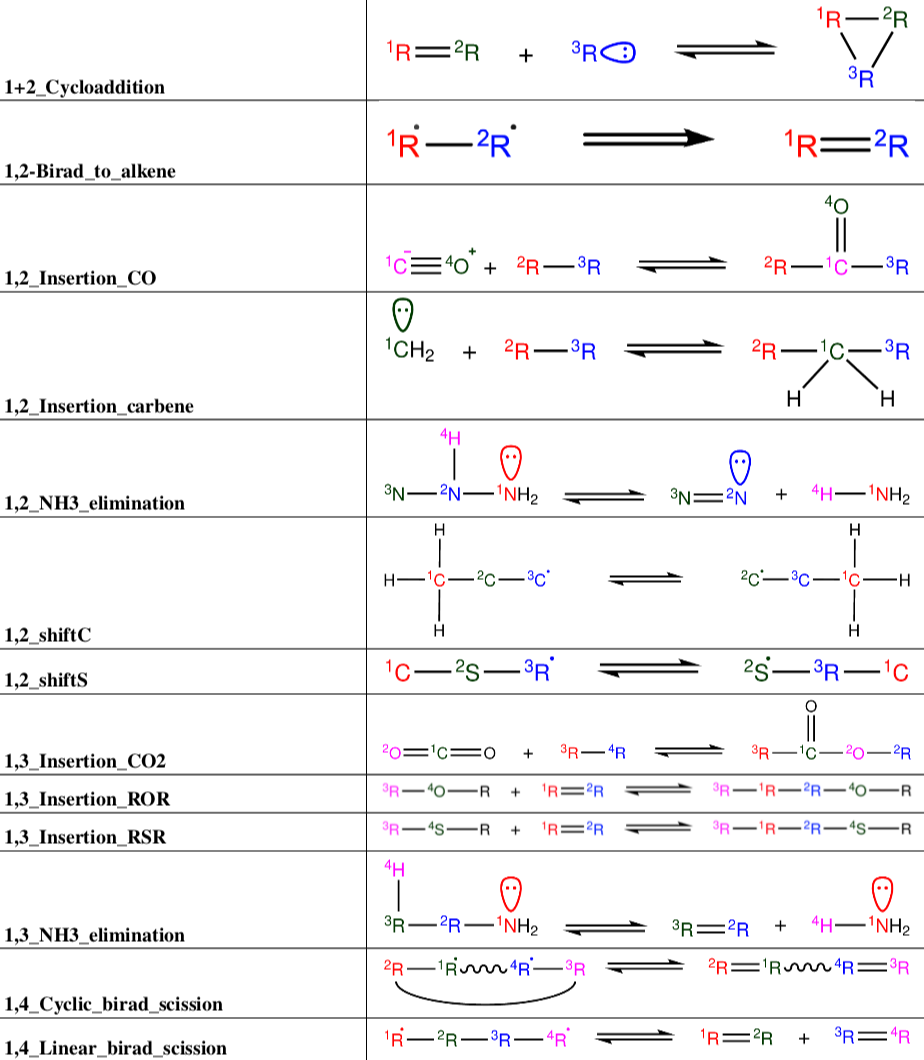
\includegraphics[scale=0.5, keepaspectratio]{images/rxn_fam1.png}
     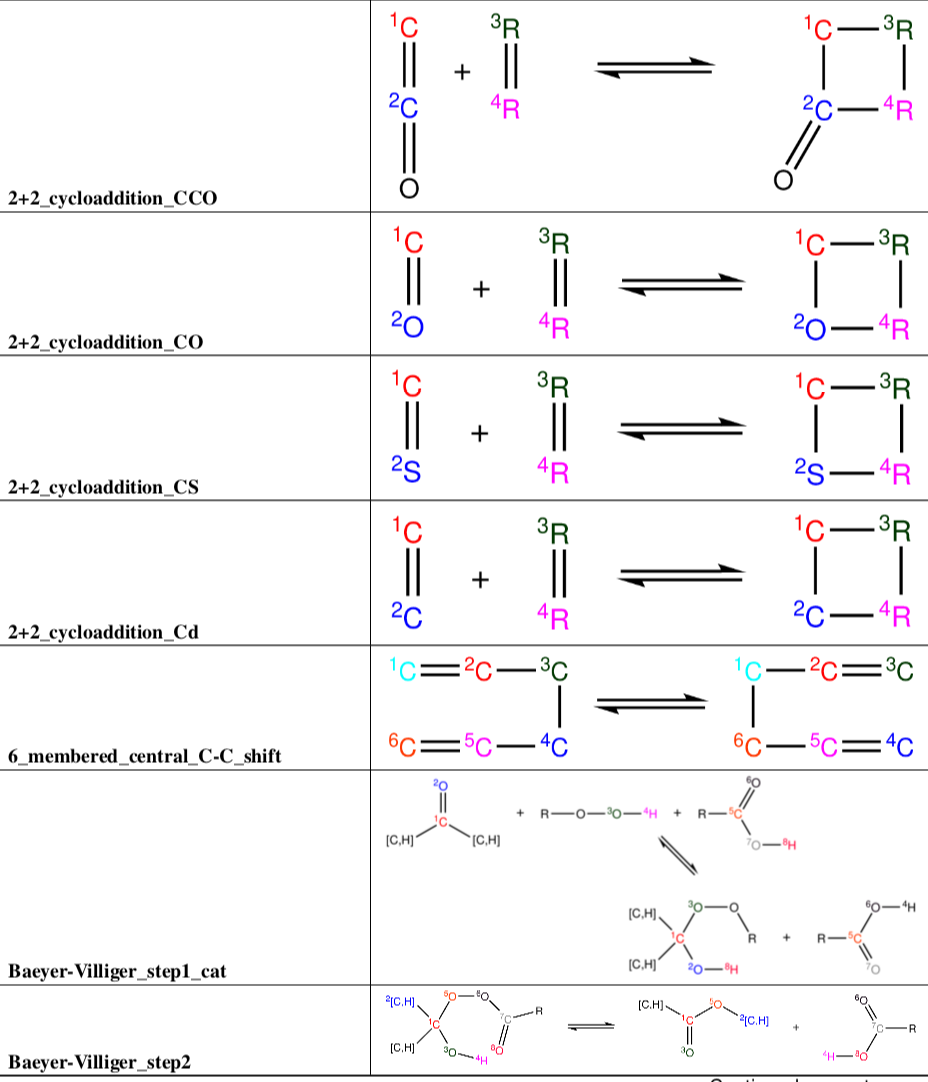
\includegraphics[scale=0.5, keepaspectratio]{images/rxn_fam2.png}
     \caption{RMG Reaction Families\cite{Gao2016ReactionMechanisms}}
     \label{fig:rxn_fam1}
 \end{figure}
 
 \begin{figure}
     \centering
     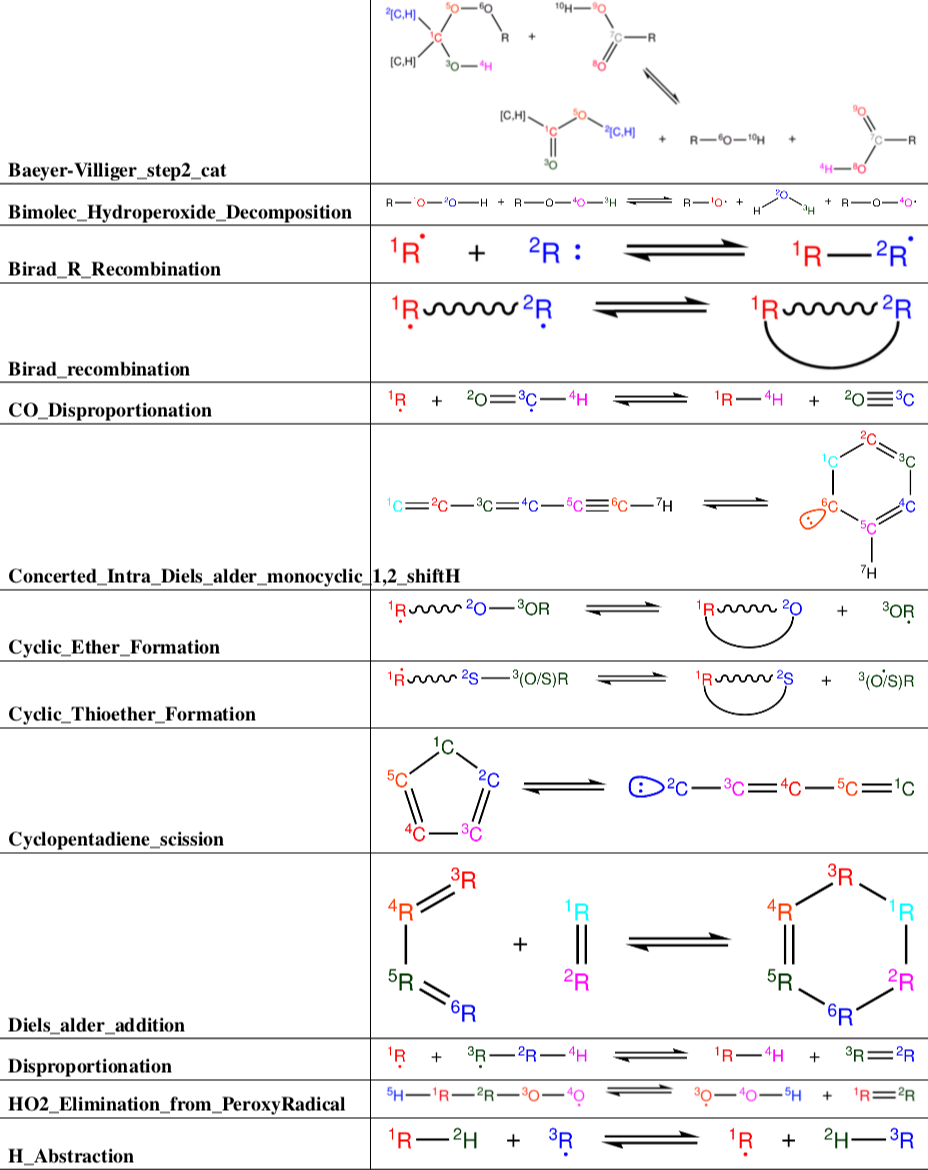
\includegraphics[scale=0.5, keepaspectratio]{images/rxn_fam3.png}
     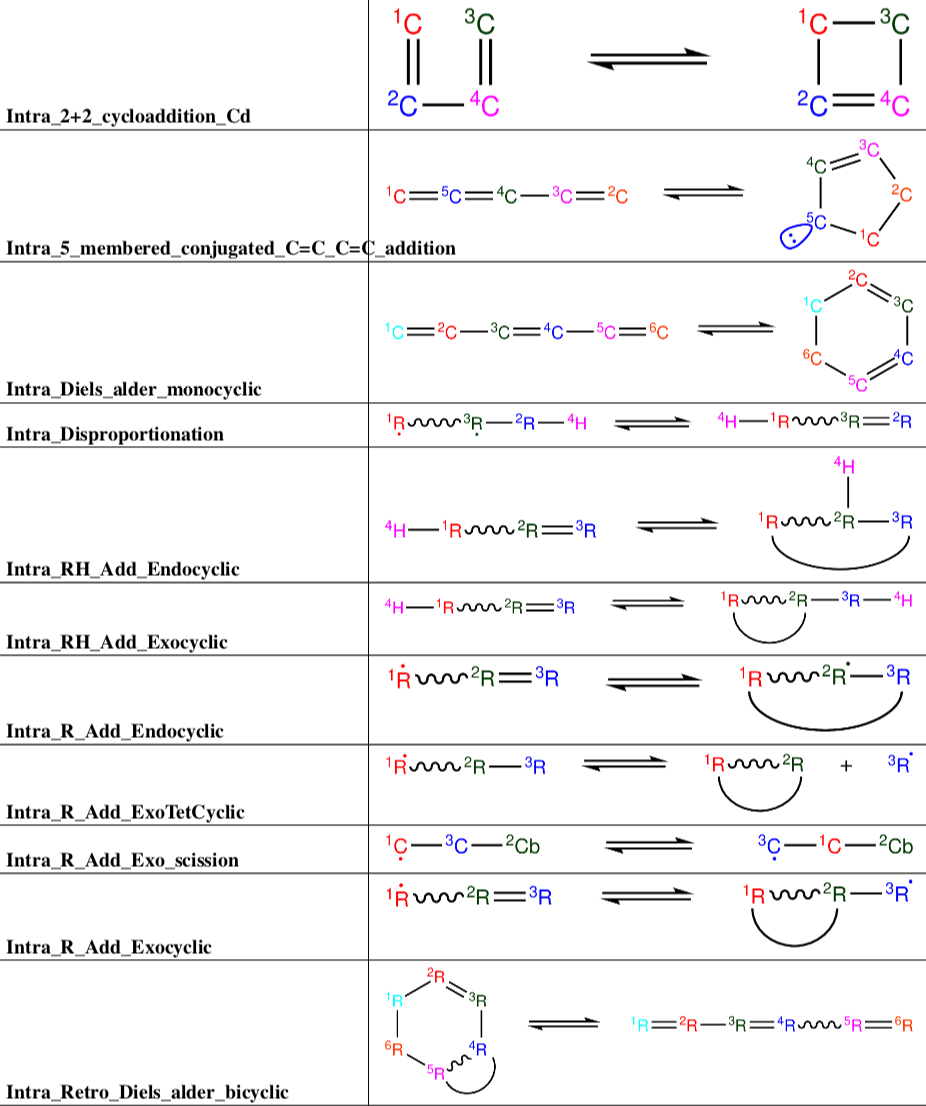
\includegraphics[scale=0.5, keepaspectratio]{images/rxn_fam4.png}
     \caption{RMG Reaction Families \cite{Gao2016ReactionMechanisms}}
     \label{fig:rxn_fam2}
 \end{figure}
 
 \begin{figure}
     \centering
     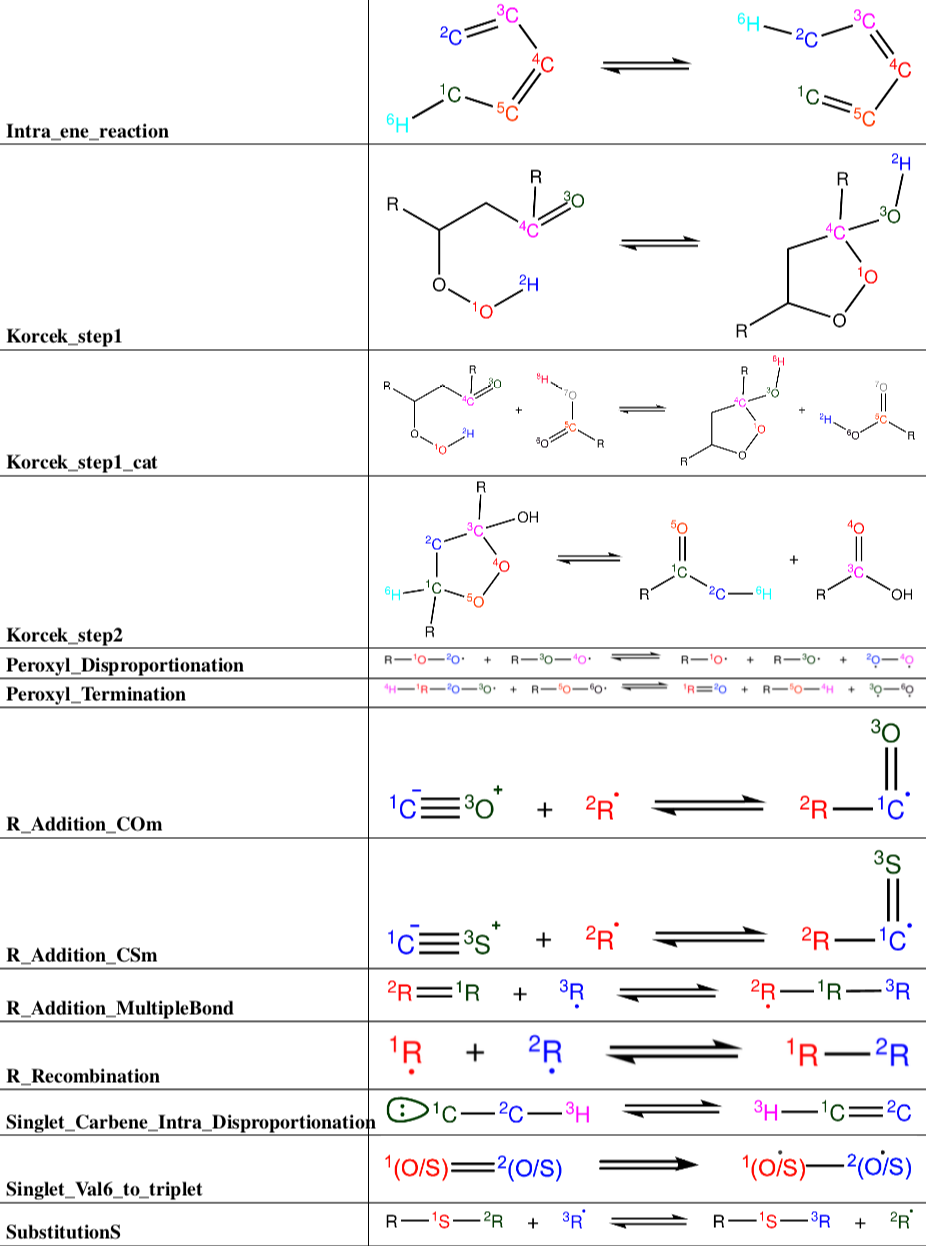
\includegraphics[scale=0.5, keepaspectratio]{images/rxn_fam5.png}
     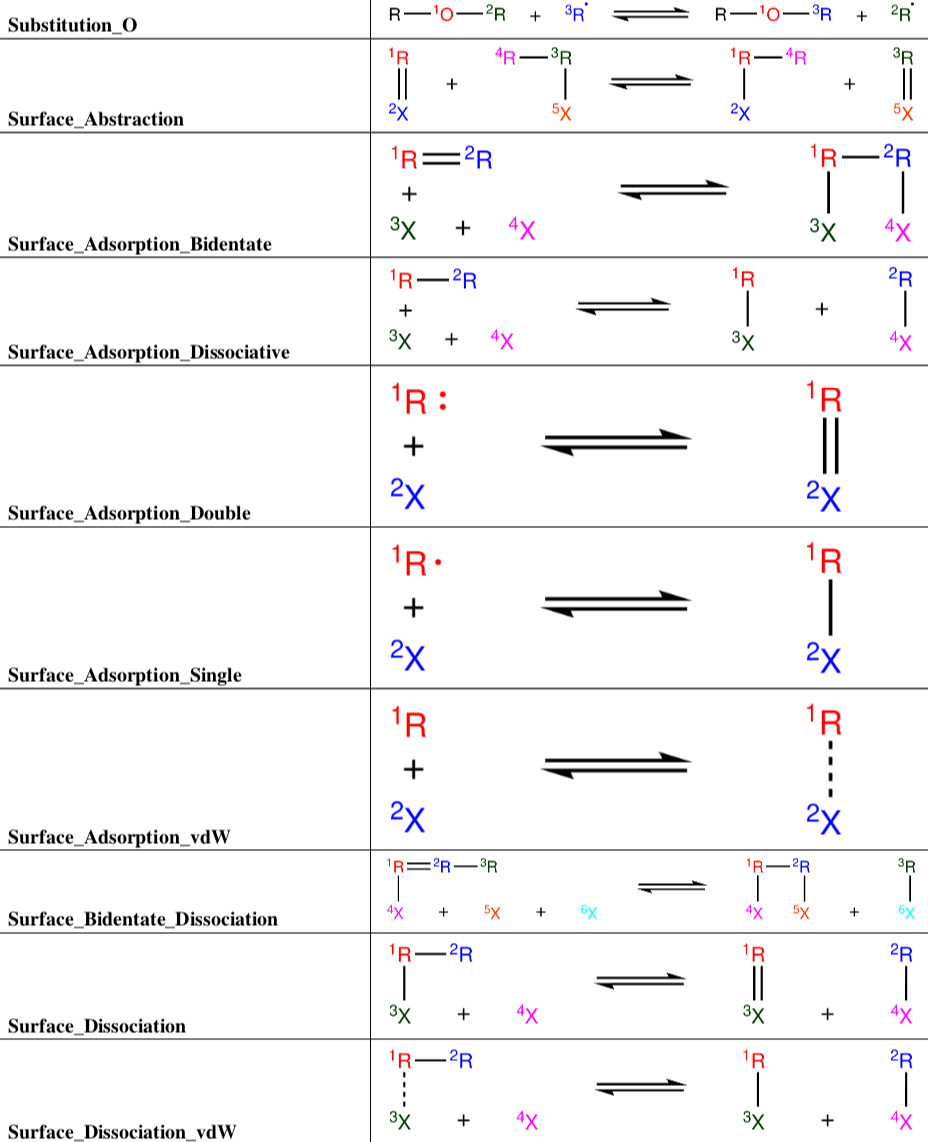
\includegraphics[scale=0.5, keepaspectratio]{images/rxn_fam6.png}
     \caption{RMG Reaction Families \cite{Gao2016ReactionMechanisms}}
     \label{fig:rxnfam3}
 \end{figure}
 \begin{figure}
     \centering
     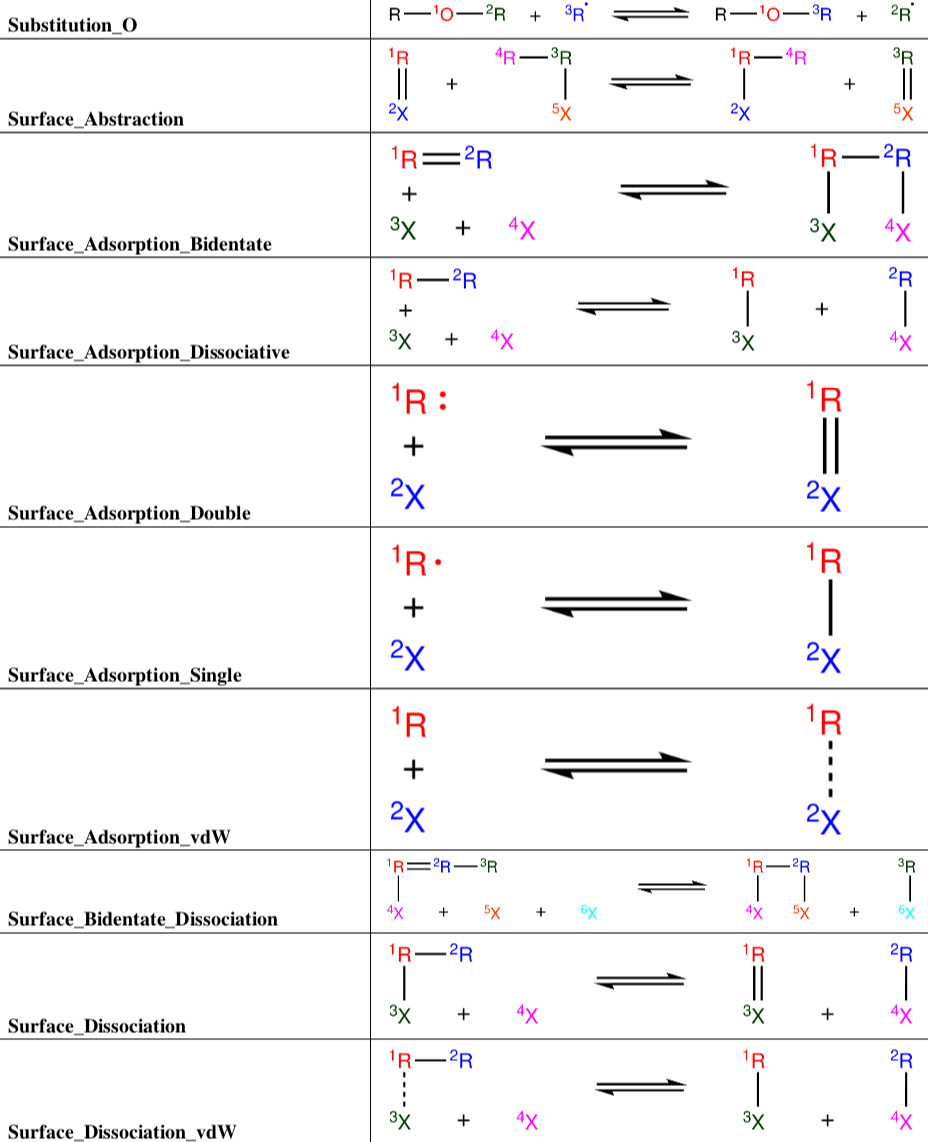
\includegraphics[scale=0.5, keepaspectratio]{images/rxn_fam6.png}
     \caption{RMG Reaction Families \cite{Gao2016ReactionMechanisms}}
     \label{fig:rxn_fam4}
 \end{figure}
 
\addcontentsline{toc}{section}{\appendixtocname}
\end{document}

\begin{document}
\clearpage
\section*{Outline}
\newcommand*{\cdone}{{\bfseries\hspace{-1.1em}{\Large{\checkmark}}\hspace{0.1em}}}
\newcommand*{\ejm}{{\hspace{-2.2em}\makebox[0pt]{\color{red}\bfseries E}}\hspace{2.2em}} % Emily

\begin{easylist}[checklist]
\ListProperties{Style*={\framebox(7,7){}}\hskip.6em}
% & \kn \ejm \cdone proposed work
& Chapter 1: Introductory Chapter
&& opening statement about the scope of this thesis and what it aims to deliver (\textbf{goal})
&&& Environmental pollution and emissions regulation around Europe and the US as indicated from the environmental protection agencies and the energy information agencies\cite{Epa2019Fast2019}\cite{EnergyInformationAdministration2018U.S.2017}
&&& The current use of fossil fuels in the form of coal, oil and natural gas for power generation, transportation and industrial processes and heavy manufacturing

&& \textbf{Goal}
&&& make the basis or set of guidelines on how to construct the most suitable surrogate models for GTL fuels that are close enough to experiments and also suitable for engine modeling. To concatenate pure primary reference fuels along with their detailed thermodynamics and kinetics or to blend all the individual species present from the onset. 
&&& This thesis dives to answer this question of which approach is the best practice to build surrogate models of GTL fuel blends and validate those models against well defined experiments as well other GTL kinetic models. In order to validate our blended models, we use a variety of experiments to verify our results. Each blend ought to have the capability of producing the detailed chemical properties of each of the main pure primary reference fuels 

&& \textbf{Motivation} 
&&& Current transportation jet fuels currently being used and the high emissions from them. 
&&& Need to replace current transportation fuels with alternatives that promise lower emissions to mitigate pollution
&&& Existing alternative transportation fuels such LNG, oxygenated fuels
&&& Short comings of the existing transportation fuels and where they fail in heavy machinery and large scale applications
&&& Need to introduce alternative transport fuels for large scale applications which do not require new engine designs, rather retrofitting our new alternative transport fuels with the existing engines
&&& Introduction of GTL fuels which have lower emissions as described by the current studies and its scalability in the near future
&&& Synthesis of GTL via the Fischer-Tropsch Process (F-T) process of carbon capture of natural gas and CO through catalytic processes and reforming
&&& Wish to reduce emissions (soot, NOx, SOx) from jet and diesel engines \cite{Boogaard2017ToxicologicalToxicology}\cite{Whale2018ToxicologicalEcotoxicology}
&&& GTL fuels are drop-in replacements (work in existing engines) with lower emissions
&&& \cdone lower soot in jet engines\cite{Wang2012}
&&& models help engine designers


&& \textbf{GTL fuels}
&&& what they are
&&& used for diesel applications, jet engines, heavy machinery
&&& fewer aromatics than petroleum diesel, so less soot
&&& made by Fischer-Tropsch catalytic conversion of \ce{CH4} to liquids (check)
&&& Need to understand how GTL fuels behave when used. 
&&&& Need to study these fuels to obtain the physical and chemical properties
&&&& Need to design experiments that closely correlates to how these fuels behave under engine-like conditions
&&&& How do we determine what makes up the GTL fuel blends
&&&& Use of mass spectrometry analysis and chromatography to see the composition of the blends
&&&& Insert charts that show the most common groups found in GTL fuel blends from the spectrometry analysis \cite{Dooley2010AProperties}
&&&& The use of surrogate fuel model blends to represent the most common groups in fuel blends 
&&&& Choice of GTL fuel blends based on Shell S-8 GTL and based on the work of \cite{Dagaut2016ExperimentalSurrogates}.


&& \textbf{Why Surrogate Models}
&&& Surrogate models allow us to properly describe complex models with the representation of just a few major fuels
&&& Surrogate models are employed in large and detailed analyses of large, complex physical domains from networks to biological systems and chemical reactivities of large compounds. The use of mass spectrometry allows us to predict which compounds are dominant in complex fuel mixtures and represent the overall mixture based on the relative proportions of the individual compounds as derived from the spectrometric analysis. 
&&& By the using surrogates, we can assume that the physical properties are closely matched to the real fuel mixture as well as the chemical properties. The physical properties include density, specific gravity, viscosity and the appropriate molecular weight of the real fuel. While that of the chemical properties attempting to match is the reacitivity of the fuel such as ignition delay times, lamianr flame speeds and species concentrations/profiles. A good surrogate fuel  should account for both the physical and chemical properties of the real fuel, especially for heavy fuels such as jet and diesel fuels, since the physcial phenomena play such an important role in the formation of air-fuel mixtures as well as soot and pollutant formation for the chemical behavior.\cite{Mehl2012ModelingApproach} 


&& \textbf{Mechanism generation}
&&& Need to design models that represent these fuels that are closely related to the real fuel
&&& Need for chemical kinetic mechanisms
&&& Detailed kinetic models that describe elementary reactions
&&& Intro to RMG \cite{Gao2016ReactionMechanisms}
&&& RMG generates them, based on reaction rules/templates, and rate estimates using group additivity, rate rules, machine learning, tree estimates.


&& Literature review: what is already known (and what is not yet) about alternative jet fuel surrogates 
&& What is known about GTL fuel surrogates and how they're constructed \cite{Naik2011DetailedFuels}\cite{Edwards2001SurrogateFuels}\cite{Dagaut2014CombustionModeling} \cite{Dooley2010AProperties}\cite{Dagaut2014}
&& GTL surrogate selection
&& GTL combustion chemistry and kinetic modeling


&& \textbf{Objective (thesis question)}:
&&& how best to build a model of a GTL fuel blend?
&&&& merge models, or build a blended model?
&&&& how do blends affect flammability ? does it improve, decrease or possibly adversely affect the flammability and what is its impact on the environment as well as engines?

& Chapter 2:Model Generation in RMG
&& how we build kinetic models
&&& how RMG works
&&&& thermo selection - group additivity and benson groups
&&&& kinetics selection - training rules and rate of flux production 
&&& surrogate molecule selection
&&&& mass spectrometry, chromatography
&&&& major compound classes are n-alkanes, iso-alkanes, naphthenes, cycloalkanes, tiny aromatics
&&&& picked representative molecules: n-decane, iso-octane, cyclo-propylhexane \cite{Chen2017ViolationModels}
&&& building models for individual components
&&&& tolerances
&&&& seed mechanisms
&&&& add species expected to be important -reaction pathways
&&&&& following reaction classes
&&&& reactor conditions
&&&&& reactor with pdep and without pdep 
&&&&& \cdone why is pdep important ? using Prof. Green's paper about temperature and molecular size of the reacting species. Using the graph of \cite{Wong2003TemperatureLimit} Fig.1, can we confidently say that it is correct to exclude the pressure dependence in the low temperature region where cool flame effects are observed. Even in Fig.3 we see the criteria for the same as regards fall off reactions and molecular size.
&&&&& temperature ranges
&&&& staging
&&&& constraints
&&& building models for mixture
&&&& concatenate models of individual components 
&&&& build a model of blended fuel
&&& Scalability Strategies \cite{Jocher2019ScalabilityGeneration}

&& Combustion chemistry
&& why is chemistry important
&& kinetics of reactions
&& high temperature combustion pathways
&&& reaction families
&&&& H abstraction
&&&& unimolecular decomposition
&& low temperature combustion pathways
&&& reaction families
&&&& H abstraction
&&&& radical isomerization

& Chapter 3: N-decane Model Generation
&& model building in RMG
&&&& thermo selection - group additivity and benson groups
&&&& kinetics selection - training rules and rate of flux production 
&&&& picked representative molecules: n-decane, iso-octane, cyclo-propylhexane \cite{Chen2017ViolationModels}
&&&& tolerances
&&&& seed mechanisms
&&&& add species expected to be important - reaction pathways\cite{Merchant2015UnderstandingPropane} path flux diagrams
&&&&& following reaction classes
&&&&& high T pathways:
&&&&& low T pathways: peroxides, ketohydroperoxides
&&&& reactor conditions
&&&&& reactor with pdep and without pdep 
&& validation of model using: 
&&& Shock Tubes for ignition delays
&&&& Rapid Compression Machines (RCM) for moving walls with imposed pressure profiles (to match Dagaut's experiments for surrogate GTL\cite{Dagaut2014})
&&& Premixed Laminar flame speeds in flow reactors
&&& Cantera comparison with other models show plots \cite{cantera}

& Chapter 4: Iso-octane Model Generation
&& model building in RMG
&&&& thermo selection - group additivity and benson groups
&&&& kinetics selection - training rules and rate of flux production 
&&&& tolerances
&&&& seed mechanisms
&&&& add species expected to be important - reaction pathways\cite{Merchant2015UnderstandingPropane} path flux diagrams
&&&&& following reaction classes
&&&&& high T pathways:
&&&&& low T pathways: peroxides, ketohydroperoxides
&&&& reactor conditions
&&&&& reactor with pdep and without pdep 
&& validation of model using: 
&&& Shock Tubes for ignition delays
&&&& Rapid Compression Machines (RCM) for moving walls with imposed pressure profiles (to match Dagaut's experiments for surrogate GTL\cite{Dagaut2014})
&&& Cantera comparison with other models show plots \cite{cantera}

& Chapter 5: Propyl-Cyclohexane Model Generation
&& model building in RMG
&&&& thermo selection - group additivity and benson groups
&&&& kinetics selection - training rules and rate of flux production 
&&&& changed kinetics by reducing A factors in the Arrhenius expressions for cyclo-propylhexane and any rate that violated the collision limit based on the approach from  \cite{Chen2017ViolationModels} and reused new rates to generate models
&&&& tolerances
&&&& seed mechanisms
&&&& add species expected to be important - reaction pathways\cite{Merchant2015UnderstandingPropane} path flux diagrams
&&&&& following reaction classes
&&&& reactor conditions
&&&&& reactor with pdep and without pdep 
&& validation of model using: 
&&& Shock Tubes for ignition delays
&&&& Rapid Compression Machines (RCM) for moving walls with imposed pressure profiles (to match Dagaut's experiments for surrogate GTL\cite{Dagaut2014})
&&& Cantera comparison with other models show plots \cite{cantera}
&&&&& high T pathways:
&&&&& low T pathways: peroxides, ketohydroperoxides occurred only for high temperature model

& Chapter 6: Blended models Model Generation
&& blended models (data from Dagaut 2014\cite{Dagaut2014}) \cite{Dooley2010MethylModel} \cite{Naik2011DetailedFuels}
&&&& ignition delays (shock tubes)
&&&& flame speeds (from burner)

& Chapter 7: Conclusions
&& Restatement of goals and motivations was thesis question answered ? 
&&& how best to build a model of a GTL fuel blend? 
&&& merge models, or build a blended model?
&&&& how do blends affect flammability ? does it improve, decrease or possibly adversely affect the flammability and what is its impact on the environment as well as engines?

&& Future Work and Recommendations
&&& Better thermo-kinetic estimates of parameters
&&& Mechanism reductions
&&& Uncertainty analysis to observe how uncertain estimates are
&&& Model generation optimization 
& Bibliography
\end{easylist}

\end{document}